%%%%%%%%%%%%%%%%%%%%%%%%%%%%%%%%%%%%%%%%%%%%%%%%%%%%%%%%%%%%%%%%%%%%%%%%%%%%%%%%
%                                                                              %
% Freyja                                                                       %
%                                                                              %
%%%%%%%%%%%%%%%%%%%%%%%%%%%%%%%%%%%%%%%%%%%%%%%%%%%%%%%%%%%%%%%%%%%%%%%%%%%%%%%%
%                                                                              %
% version: 2016-05-18T1201Z                                                    %
%                                                                              %
%%%%%%%%%%%%%%%%%%%%%%%%%%%%%%%%%%%%%%%%%%%%%%%%%%%%%%%%%%%%%%%%%%%%%%%%%%%%%%%%
%                                                                              %
% DESCRIPTION                                                                  %
%                                                                              %
% This program can be used to create Beamer slides. It demonstrates various    %
% presentations of information, including itemised lists with checkmarks,      %
% syntax-highlighted code, static images, animated images and embedded data.   %
%                                                                              %
% CONFIGURATION                                                                %
%                                                                              %
% Slide styles and various other settings can be selected using the            %
% configuration section. For example, to set the style to greyscale, use the   %
% following setting:                                                           %
%                                                                              %
%     \edef\style{1}                                                           %
%                                                                              %
%%%%%%%%%%%%%%%%%%%%%%%%%%%%%%%%%%%%%%%%%%%%%%%%%%%%%%%%%%%%%%%%%%%%%%%%%%%%%%%%
%                                                                              %
% LICENCE INFORMATION                                                          %
%                                                                              %
% This program produces Beamer slides.                                         %
%                                                                              %
% copyright (C) 2013 William Breaden Madden                                    %
%                                                                              %
% This software is released under the terms of the GNU General Public License  %
% version 3 (GPLv3).                                                           %
%                                                                              %
% This program is free software: you can redistribute it and/or modify it      %
% under the terms of the GNU General Public License as published by the Free   %
% Software Foundation, either version 3 of the License, or (at your option)    %
% any later version.                                                           %
%                                                                              %
% This program is distributed in the hope that it will be useful, but WITHOUT  %
% ANY WARRANTY; without even the implied warranty of MERCHANTABILITY or        %
% FITNESS FOR A PARTICULAR PURPOSE. See the GNU General Public License for     %
% more details.                                                                %
%                                                                              %
% For a copy of the GNU General Public License, see                            %
% <http://www.gnu.org/licenses/>.                                              %
%                                                                              %
%%%%%%%%%%%%%%%%%%%%%%%%%%%%%%%%%%%%%%%%%%%%%%%%%%%%%%%%%%%%%%%%%%%%%%%%%%%%%%%%

\documentclass[american, xcolor=dvipsnames]{beamer}
% strikethrough
    \usepackage[normalem]{ulem}

%%%%%%%%%%%%%%%%%%%%%%%%%%%%%%%%%%%%%%%%%%%%%%%%%%%%%%%%%%%%%%%%%%%%%%%%%%%%%%%%
%                                                                              %
% CONFIGURATION                                                                %
%                                                                              %
% - style                                                                      %
%     - terminal green:      0                                                 %
%     - greyscale:           1                                                 %
%     - CERN                 2                                                 %
% - institution                                                                %
%     - UoG:                 0                                                 %
%     - CERN                 1                                                 %
% - code listings style                                                        %
%     - color                0                                                 %
%     - greyscale            1                                                 %
% - aspect ratio                                                               %
%     - widescreen:          0                                                 %
%     - four-by-three:       1                                                 %
%     - golden ratio:        2                                                 %
% - outline                                                                    %
%     - on:                  0                                                 %
%     - off:                 1                                                 %
% - headline contents                                                          %
%     - on:                  0                                                 %
%     - off:                 1                                                 %
% - footline                                                                   %
%     - on:                  0                                                 %
%     - off:                 1                                                 %
%                                                                              %
%%%%%%%%%%%%%%%%%%%%%%%%%%%%%%%%%%%%%%%%%%%%%%%%%%%%%%%%%%%%%%%%%%%%%%%%%%%%%%%%

%%%%%%%%%%%%%%%%%%%%%%%%%%%%%%%%%%%%%%%%%%%%%%%%%%%%%%%%%%%%%%%%%%%%%%%%%%%%%%%%
% titles, authors and institutions specifications                              %
%%%%%%%%%%%%%%%%%%%%%%%%%%%%%%%%%%%%%%%%%%%%%%%%%%%%%%%%%%%%%%%%%%%%%%%%%%%%%%%%

\newcommand{\titleSpecification}{
    quick update
}
\newcommand{\titlePageTitleSpecification}{
    \LARGE QUICK UPDATE\\
    \large ${8\textrm{ TeV}}$--${13\textrm{ TeV}}$ comparisons
}
\newcommand{\authorSpecification}{
    \sout{G.~Aad~et.~al.} \underline{Number~6}, Number~1
}
\newcommand{\instituteSpecification}{
    University~of~Glasgow
}

%%%%%%%%%%%%%%%%%%%%%%%%%%%%%%%%%%%%%%%%%%%%%%%%%%%%%%%%%%%%%%%%%%%%%%%%%%%%%%%%
% style settings                                                               %
%%%%%%%%%%%%%%%%%%%%%%%%%%%%%%%%%%%%%%%%%%%%%%%%%%%%%%%%%%%%%%%%%%%%%%%%%%%%%%%%

\edef\style{2}
\edef\institution{0}
\edef\codeStyle{0}
\edef\aspectRatio{0}
\edef\titlePage{1}
\edef\outlineSpecification{0}
\edef\headlineContents{0}
\edef\footline{1}

%%%%%%%%%%%%%%%%%%%%%%%%%%%%%%%%%%%%%%%%%%%%%%%%%%%%%%%%%%%%%%%%%%%%%%%%%%%%%%%%
% measures specifications                                                      %
%%%%%%%%%%%%%%%%%%%%%%%%%%%%%%%%%%%%%%%%%%%%%%%%%%%%%%%%%%%%%%%%%%%%%%%%%%%%%%%%

\newcommand{\measureJSpecification}{1 cm}
\newcommand{\measureKSpecification}{2 cm}
\newcommand{\measureLSpecification}{3 cm}
\newcommand{\measureMSpecification}{4 cm}
\newcommand{\measureNSpecification}{5.5 cm}
\newcommand{\measureOSpecification}{5 cm}
\newcommand{\measurePSpecification}{6 cm}
\newcommand{\measureQSpecification}{7 cm}
\newcommand{\measureRSpecification}{8 cm}
\newcommand{\measureSSpecification}{9 cm}
\newcommand{\measureTSpecification}{10 cm}
\newcommand{\measureUSpecification}{11 cm}

%%%%%%%%%%%%%%%%%%%%%%%%%%%%%%%%%%%%%%%%%%%%%%%%%%%%%%%%%%%%%%%%%%%%%%%%%%%%%%%%
% end of configuration                                                         %
%%%%%%%%%%%%%%%%%%%%%%%%%%%%%%%%%%%%%%%%%%%%%%%%%%%%%%%%%%%%%%%%%%%%%%%%%%%%%%%%


% aspect ratio
    \ifcase\aspectRatio
        % case 0 (widescreen)
        \usepackage[
            width=16,
            height=9,
            orientation=landscape,
            size=custom,
            scale=0.5,
            debug
         ]{beamerposter}
    \or
        % case 1 (four-by-three)
        \usepackage[
            width=16,
            height=12,
            orientation=landscape,
            size=custom,
            scale=0.5,
            debug
        ]{beamerposter}
    \or
        % case 2 (golden ratio)
        \usepackage[
            width=16,
            height=9.89,
            orientation=landscape,
            size=custom,
            scale=0.5,
            debug
        ]{beamerposter}
    \fi
% graphics
    \usepackage{graphicx}
    \usepackage{pgf}
    \usepackage{tikz}
    \usetikzlibrary{arrows, automata}
    \usetikzlibrary{shapes, arrows}
    \usetikzlibrary{positioning}
    \usepackage{fancyvrb}
% mathematics
    \usepackage{amsmath}
    \def\evaluate#1{\the\numexpr#1\relax}
% floor and ceiling functions
% examples:
% - \ceil{x}
% - \ceil[\big]{x}
% - \ceil[\Big]{x}
% - \ceil[\bigg]{x}
% - \ceil[\Bigg]{x}
% (and similar for \floor)
    \usepackage{mathtools}
    \usetikzlibrary{fit, arrows, calc, positioning}
    \DeclarePairedDelimiter{\ceil}{\lceil}{\rceil}
    \DeclarePairedDelimiter{\floor}{\lfloor}{\rfloor}
% checklists
    \usepackage{bbding}
% hyperlinks
    \usepackage{hyperref}
% verbatim
    \usepackage{verbatim}
% justification
    \usepackage{ragged2e}
% Lorem ipsum
    \usepackage{lipsum}
% multiple columns
    \usepackage{multicol}
% textblock
    \usepackage{textpos}
% time
% ISO date
    \usepackage{babel}
% date formatting
    \usepackage{datetime}
    \newdateformat{timeA}{
        \THEYEAR-\twodigit{\THEMONTH}-\twodigit{\THEDAY}
    }
    \newdateformat{timeB}{
        \THEDAY~\monthname[\THEMONTH] \THEYEAR
    }
    \newdateformat{timeC}{
        \monthname[\THEMONTH] \THEYEAR
    }
    \newtimeformat{timeD}{%
        \twodigit{\THEHOUR}\twodigit{\THEMINUTE}\twodigit{\THESECOND}
    }
    \newtimeformat{timeE}{%
        \twodigit{\THEHOUR}\twodigit{\THEMINUTE}
    }
    \newdateformat{timeF}{
        \THEYEAR-\twodigit{\THEMONTH}-\twodigit{\THEDAY}T\timeD
    }
    \newdateformat{timeG}{
        \THEYEAR-\twodigit{\THEMONTH}-\twodigit{\THEDAY}T\timeE
    }
% tables
    \usepackage{multirow}
% media and animation
    \usepackage{multimedia}
    \usepackage{animate}
% embed
    \usepackage{attachfile}
% colors
    \usepackage{color}
    % greyscale
        % black
            \definecolor{black1}{RGB}{0, 0, 0}
        % white
            \definecolor{white1}{RGB}{255, 255, 255}
        % light grey
            \definecolor{greyLight1}{RGB}{153, 153, 153}
        % dark grey
            \definecolor{greyDark1}{RGB}{64, 64, 64}
    % blues
        \definecolor{blue1}{RGB}{0, 0, 255}
        \definecolor{blueLight1}{RGB}{85, 85, 255}
        \definecolor{blueLight2}{RGB}{170, 170, 255}
        \definecolor{blueDark1}{RGB}{0, 0, 170}
        % grey blue
            \definecolor{greyBlue1}{RGB}{254, 254, 10}
        % CERN blue
            \definecolor{CERNBlue1}{RGB}{0, 83, 161}
            \definecolor{CERNBlueLight1}{RGB}{0, 103, 200}
            \definecolor{CERNBlueDark1}{RGB}{0, 63, 122}
    % turquoise
        \definecolor{turquoise1}{RGB}{64, 224, 208}
    % greens
        \definecolor{green1}{RGB}{0, 255, 0}
        \definecolor{greenLight1}{RGB}{85, 255, 85}
        \definecolor{greenDark1}{RGB}{0, 170, 0}
        % terminal green
            \definecolor{terminalGreen1}{RGB}{0, 255, 0}
        % terminal green light
            \definecolor{terminalGreenLight1}{RGB}{55, 200, 55}
        % terminal green dark
            \definecolor{terminalGreenDark1}{RGB}{0, 200, 0}
    % yellows
        % plasma yellow (GRiD Compass)
            \definecolor{plasmaYellow1}{RGB}{254, 254, 10}
    % reds
        \definecolor{red1}{RGB}{255, 0, 0}
        \definecolor{redLight1}{RGB}{255, 85, 85}
        \definecolor{redDark1}{RGB}{170, 0, 0}
% theme
    % set base theme
        \usetheme{Warsaw}
    % headline contents
        \ifcase\headlineContents
            % case 0
            \setbeamertemplate{headline}{}
        \or
            % case 1
            %\setbeamertemplate{headline}{}
        \fi
    % footline
        \ifcase\footline
            % case 0
            \setbeamertemplate{footline}{}
        \or
            % case 1
            %\setbeamertemplate{footline}{}
        \fi
    % set navigation icons off
        \setbeamertemplate{navigation symbols}{}
    % boxes
        % set title box to rectangular without shadow
            \setbeamertemplate{title page}[default][rounded=false, shadow=false]
        % set shadows on boxes off
        \setbeamertemplate{blocks}[rounded][shadow=true]
            \setbeamertemplate{blocks}[rounded=false, shadow=false]
        % list marker types
            % set list marker types (e.g., ball, circle, rectangle, default)
                \setbeamertemplate{items}[circle]
                \setbeamertemplate{itemize subitem}[circle]
            % set table of contents list marker types
                \setbeamertemplate{section in toc}[circle]
                \setbeamertemplate{subsection in toc}[circle]
    % set shadows on header off
        \setbeamertemplate{frametitle}[default][rounded=false, shadow=false]
    % colors
        \ifcase\style
            % case 0
            % set palettes
                \setbeamercolor*{palette primary}{
                    use=structure,
                    fg=black1,
                    bg=terminalGreen1
                }
                \setbeamercolor*{palette quaternary}{
                    fg=terminalGreen1,
                    bg=black1
                }
            % set foreground color
                \setbeamercolor{normal text}{fg=terminalGreen1}		
            % set background color
                \setbeamercolor{normal text}{bg=black1}	
            % set block colors and appearance
                \setbeamercolor{block title}{
                    bg=terminalGreen1,
                    fg=black1
                }
                \setbeamercolor{block body}{
                    bg=black1,
                    fg=terminalGreen1
                }
                \setbeamertemplate{blocks}[rounded=false, shadow=false]
            % set table of contents list marker colors
                \setbeamercolor{section number projected}{
                    bg=terminalGreen1,
                    fg=black1
                }
            % set description list marker colors
                \setbeamercolor{description item}{
                    bg=black1,
                    fg=terminalGreen1
                }
                \setbeamercolor{description subitem}{
                    bg=black1,
                    fg=terminalGreen1
                }
                \setbeamercolor{description subsubitem}{
                    bg=black1,
                    fg=terminalGreen1
                }
            % set itemized list marker colors
                \setbeamercolor{itemize item}{
                    bg=black1,
                    fg=terminalGreen1
                }
                \setbeamercolor{itemize subitem}{
                    bg=black1,
                    fg=terminalGreen1
                }
                \setbeamercolor{itemize subsubitem}{
                    bg=black1,
                    fg=terminalGreen1
                }
            % set enumerated list marker colors
                \setbeamercolor{item projected}{
                    bg=black1,
                    fg=terminalGreen1
                }
            % set table of contents section colors
                \setbeamercolor{section in toc}{
                    bg=terminalGreen1,
                    fg=black1
                }
            % hyperlinks
                \hypersetup{
                    colorlinks=true,
                    linkcolor=,
                    urlcolor=terminalGreenLight1
                }
            % emoticons
                \newcommand{\emoticonsColor}{terminalGreen1}
            % text highlighting
                \newcommand{\highlightA}[1]{\colorbox{terminalGreenLight1}{#1}}
        \or
            % case 1
            % set palettes
                \setbeamercolor*{palette primary}{
                    use=structure,
                    fg=white1,
                    bg=greyLight1
                }
                \setbeamercolor*{palette quaternary}{
                    fg=white1,
                    bg=greyDark1
                }
            % set background color
                \setbeamercolor{normal text}{bg=black1}
            % set foreground color
                \setbeamercolor{normal text}{fg=white1}
            % set block colors and appearance
                \setbeamercolor{block title}{
                    bg=greyLight1,
                    fg=white1
                }
                \setbeamercolor{block body}{
                    bg=white1,
                    fg=greyLight1
                }
                \setbeamertemplate{blocks}[rounded=false, shadow=false]
            % set table of contents list marker colors
                \setbeamercolor{section number projected}{
                    bg=greyLight1,
                    fg=white1
                }
            % set description list marker colors
                \setbeamercolor{description item}{
                    bg=greyLight1,
                    fg=white1
                }
                \setbeamercolor{description subitem}{
                    bg=greyLight1,
                    fg=white1
                }
                \setbeamercolor{description subsubitem}{
                    bg=greyLight1,
                    fg=white1
                }
            % set itemized list marker colors
                \setbeamercolor{itemize item}{
                    bg=greyLight1,
                    fg=white1
                }
                \setbeamercolor{itemize subitem}{
                    bg=greyLight1,
                    fg=white1
                }
                \setbeamercolor{itemize subsubitem}{
                    bg=greyLight1,
                    fg=white1
                }
            % set enumerated list marker colors
                \setbeamercolor{item projected}{
                    bg=greyLight1,
                    fg=white1
                }
            % set table of contents section colors
                \setbeamercolor{section in toc}{
                    bg=greyLight1,
                    fg=white1
                }
            % hyperlinks
                \hypersetup{
                    colorlinks=true,
                    linkcolor=,
                    urlcolor=greyLight1
                }
            % emoticons
                \newcommand{\emoticonsColor}{white1}
            % text highlighting
                \newcommand{\highlightA}[1]{\colorbox{greyLight1}{#1}}
        \or
            % case 2
            % set palettes
                \setbeamercolor*{palette primary}{
                    use=structure,
                    fg=white1,
                    bg=CERNBlue1
                }
                \setbeamercolor*{palette quaternary}{
                    fg=white1,
                    bg=CERNBlue1
                }
            % set background color
                \setbeamercolor{normal text}{bg=white1}
            % set foreground color
                \setbeamercolor{normal text}{fg=CERNBlue1}
            % set block colors and appearance
                \setbeamercolor{block title}{
                    bg=greyLight1,
                    fg=white1
                }
                \setbeamercolor{block body}{
                    bg=CERNBlue1,
                    fg=white1
                }
                \setbeamertemplate{blocks}[rounded=false, shadow=false]
            % set table of contents list marker colors
                \setbeamercolor{section number projected}{
                    bg=white1,
                    fg=CERNBlue1
                }
            % set description list marker colors
                \setbeamercolor{description item}{
                    bg=white1,
                    fg=CERNBlue1
                }
                \setbeamercolor{description subitem}{
                    bg=white1,
                    fg=CERNBlue1
                }
                \setbeamercolor{description subsubitem}{
                    bg=white1,
                    fg=CERNBlue1
                }
            % set itemized list marker colors
                \setbeamercolor{itemize item}{
                    bg=white1,
                    fg=CERNBlue1
                }
                \setbeamercolor{itemize subitem}{
                    bg=white1,
                    fg=CERNBlue1
                }
                \setbeamercolor{itemize subsubitem}{
                    bg=white1,
                    fg=CERNBlue1
                }
            % set enumerated list marker colors
                \setbeamercolor{item projected}{
                    bg=white1,
                    fg=CERNBlue1
                }
            % set table of contents section colors
                \setbeamercolor{section in toc}{
                    bg=white1,
                    fg=CERNBlue1
                }
            % hyperlinks
                \hypersetup{
                    colorlinks=true,
                    linkcolor=,
                    urlcolor=CERNBlueDark1
                }
            % emoticons
                \newcommand{\emoticonsColor}{CERNBlue1}
            % text highlighting
                \newcommand{\highlightA}[1]{\colorbox{CERNBlueLight1}{#1}}
        \fi
% logo
    \ifcase\style
        % case 0
            % UoG
                \newcommand\logoAFile{{\directoryImagesA/logo_UoG_green.png}}
                \newcommand{\logoAHeightSpecification}{0.5 cm}
                \newcommand{\logoBHeightSpecification}{6 cm}
    \or
        % case 1
            % UoG
                \newcommand\logoAFile{{\directoryImagesA/logo_UoG_grey.png}}
                \newcommand{\logoAHeightSpecification}{0.5 cm}
                \newcommand{\logoBHeightSpecification}{6 cm}
    \or
        % case 2
            \ifcase\institution
                % case 0 (UoG)
                    \newcommand\logoAFile{{\directoryImagesA/logo_UoG_CERN_blue.png}}
                    \newcommand{\logoAHeightSpecification}{0.5 cm}
                    \newcommand{\logoBHeightSpecification}{6 cm}
            \or
                % case 1 (CERN)
                    \newcommand\logoAFile{{\directoryImagesA/LogoOutline-Blue-04.png}}
                    \newcommand{\logoAHeightSpecification}{0.7 cm}
                    \newcommand{\logoBHeightSpecification}{2.5 cm}
            \or
                % case 2 (ATLAS)
                    \newcommand\logoAFile{{\directoryImagesA/ATLAS_logo_CERN_blue.png}}
                    \newcommand{\logoAHeightSpecification}{0.9 cm}
                    \newcommand{\logoBHeightSpecification}{3.5 cm}
            \fi
    \fi
% syntax highlighting
    \usepackage{listings}
    % default fixed font does not support bold face
        \DeclareFixedFont{\ttb}{T1}{txtt}{bx}{n}{12} % bold
        \DeclareFixedFont{\ttm}{T1}{txtt}{m}{n}{12} % normal
    % Python
        % style for highlighting
            \ifcase\codeStyle
            % case 0 (color code)
                \newcommand\pythonstyle{\lstset{
                    language=Python,
                    % colors
                        %backgroundcolor=\color{black},
                    % font
                        % general
                            basicstyle=\ttfamily\footnotesize,
                        % directive
                            %directivestyle={\color{orange}},
                        % emphasis
                            emph={MyClass, __init__},
                            emphstyle={\ttb\color{redLight1}},
                        % keywords
                            keywordstyle={\color{blueLight2}},
                            otherkeywords={self,},
                        % strings
                            stringstyle=\color{greenLight1},
                        % comments
                            commentstyle=\color{yellow}\ttfamily,
                            morecomment=[l][\color{orange}]{\#},
                    % whitespace
                        % underscores
                            showspaces=false,
                            showstringspaces=false,
                        % tabs
                            showtabs=false,
                            tabsize=2,
                    % line numbers
                        % presence and position
                            %numbers=left,
                        % font size
                            numberstyle=\footnotesize,
                        % step between two line numbers
                            stepnumber=1,
                        % distance from code
                            numbersep=10pt,
                    % comment within code
                        escapeinside={\%*}{*)},
                    % wrapping
                        % automatic line breaking
                            breaklines=true,
                        % automatic line breaking only at whitespace
                            breakatwhitespace=false,
                    % frame
                        %frame=single,
                        %frame=tb,
                    % caption
                        %caption="code"
                        % caption position (bottom)
                        captionpos=b,
                }}
            % environment
                \lstnewenvironment{python}[1][]{
                    \pythonstyle
                    \lstset{#1}
                }{}
            % for external files
                \newcommand\pythonexternal[1]{{
                    \pythonstyle
                    \lstinputlisting{#1}}
                }
            % for inline
                \newcommand\pythoninline[1]{{
                    \pythonstyle
                    \lstinline!#1!
                }}
            \fi
    % LaTeX
        % style for highlighting
            \ifcase\codeStyle
            % case 0 (color code)
                \newcommand\latexstyle{\lstset{
                    language=TeX,
                    % colors
                        %backgroundcolor=\color{black},
                    % font
                        % general
                            basicstyle=\ttfamily\footnotesize,
                        % directive
                            directivestyle={\color{orange}},
                        % emphasis
                            emph={},
                            emphstyle={\ttb\color{redLight1}},
                        % keywords
                            keywordstyle={\color{blueLight2}},
                            otherkeywords={self,},
                        % strings
                            stringstyle=\color{greenLight1},
                        % comments
                            commentstyle=\color{yellow}\ttfamily,
                            morecomment=[l][\color{orange}]{\#},
                    % whitespace
                        % underscores
                            showspaces=false,
                            showstringspaces=false,
                        % tabs
                            showtabs=false,
                            tabsize=2,
                    % line numbers
                        % presence and position
                            %numbers=left,
                        % font size
                            numberstyle=\footnotesize,
                        % step between two line numbers
                            stepnumber=1,
                        % distance from code
                            numbersep=10pt,
                    % comment within code
                        escapeinside={\%*}{*)},
                    % wrapping
                        % automatic line breaking
                            breaklines=true,
                        % automatic line breaking only at whitespace
                            breakatwhitespace=false,
                    % frame
                        %frame=single,
                        %frame=tb,
                    % caption
                        %caption="code"
                        % caption position (bottom)
                        captionpos=b,
                }}
            % environment
                \lstnewenvironment{latex}[1][]{
                    \latexstyle
                    \lstset{#1}
                }{}
            % for external files
                \newcommand\latexexternal[1]{{
                    \latexstyle
                    \lstinputlisting{#1}}
                }
            % for inline
                \newcommand\latexinline[1]{{
                    \latexstyle
                    \lstinline!#1!
                }}
            \fi
    % C++
        % style for highlighting
            \ifcase\codeStyle
            % case 0 (color code)
                \newcommand\cppstyle{\lstset{
                    language=C++,
                    % colors
                        %backgroundcolor=\color{black},
                    % font
                        % general
                            basicstyle=\ttfamily\footnotesize,
                        % directive
                            directivestyle={\color{orange}},
                        % emphasis
                            emph={int, char, double, float, unsigned},
                            emphstyle={\ttb\color{redLight1}},
                        % keywords
                            keywordstyle={\color{blueLight2}},
                            otherkeywords={$, \{, \}, \[, \]},
                        % strings
                            stringstyle=\color{greenLight1},
                        % comments
                            commentstyle=\color{yellow}\ttfamily,
                            morecomment=[l][\color{orange}]{\#}
                    % whitespace
                        % underscores
                            showspaces=false,
                            showstringspaces=false,
                        % tabs
                            showtabs=false,
                            tabsize=2,
                    % line numbers
                        % presence and position
                            %numbers=left,
                        % font size
                            numberstyle=\footnotesize,
                        % step between two line numbers
                            stepnumber=1,
                        % distance from code
                            numbersep=10pt,
                    % comment within code
                        escapeinside={\%*}{*)},
                    % wrapping
                        % automatic line breaking
                            breaklines=true,
                        % automatic line breaking only at whitespace
                            breakatwhitespace=false,
                    % frame
                        %frame=single,
                        %frame=tb,
                    % caption
                        %caption="code"
                        % caption position (bottom)
                        captionpos=b,
                }}
            \or
            % case 1 (greyscale code)
                \newcommand\cppstyle{\lstset{
                    language=C++,
                    % colors
                        %backgroundcolor=\color{darkgray},
                    % font
                        % general
                            basicstyle=\ttfamily\footnotesize,
                        % directive
                            %directivestyle={\color{<color>}},
                        % emphasis
                            emph={int, char, double, float, unsigned},
                            %emphstyle={\ttb\color{<color>}},
                        % keywords
                            %keywordstyle={\color{blue1}},
                            otherkeywords={$, \{, \}, \[, \]},
                        % strings
                            %stringstyle=\color{<color>},
                        % comments
                            %commentstyle=\color{<color>}\ttfamily,
                            %morecomment=[l][\color{<color>}]{\#}
                    % whitespace
                        % underscores
                            showspaces=false,
                            showstringspaces=false,
                        % tabs
                            showtabs=false,
                            tabsize=2,
                    % line numbers
                        % presence and position
                            %numbers=left,
                        % font size
                            numberstyle=\footnotesize,
                        % step between two line numbers
                            stepnumber=1,
                        % distance from code
                            numbersep=10pt,
                    % comment within code
                        escapeinside={\%*}{*)},
                    % wrapping
                        % automatic line breaking
                            breaklines=true,
                        % automatic line breaking only at whitespace
                            breakatwhitespace=false,
                    % frame
                        %frame=single,
                        %frame=tb,
                    % caption
                        %caption="code"
                        % caption position (bottom)
                        captionpos=b,
                }}
            \fi
        % environment
            \lstnewenvironment{cpp}[1][]{
                \cppstyle
                \lstset{#1}
            }{}
        % for external files
            \newcommand\cppexternal[1]{{
                \cppstyle
                \lstinputlisting{#1}}
            }
        % for inline
            \newcommand\cppinline[1]{{
                \cppstyle
                \lstinline!#1!
            }}
% emoticons
\newcommand{\smiley}{\tikz[baseline=-0.75ex, \emoticonsColor]{
    \draw circle (2mm);
    \node[fill,circle,inner sep=0.5pt] (left eye) at (135:0.8mm) {};
    \node[fill,circle,inner sep=0.5pt] (right eye) at (45:0.8mm) {};
    \draw (-145:0.9mm) arc (-120:-60:1.5mm);
}}
\newcommand{\frownie}{\tikz[baseline=-0.75ex, \emoticonsColor]{
    \draw circle (2mm);
    \node[fill,circle,inner sep=0.5pt] (left eye) at (135:0.8mm) {};
    \node[fill,circle,inner sep=0.5pt] (right eye) at (45:0.8mm) {};
    \draw (-145:0.9mm) arc (120:60:1.5mm);
}}
\newcommand{\neutralie}{\tikz[baseline=-0.75ex, \emoticonsColor]{
    \draw circle (2mm);
    \node[fill,circle,inner sep=0.5pt] (left eye) at (135:0.8mm) {};
    \node[fill,circle,inner sep=0.5pt] (right eye) at (45:0.8mm) {};
    \draw (-135:0.9mm) -- (-45:0.9mm);
}}
% tape symbol
    % tape symbol package
        \usepackage{bbding}
    % Use relsize for the raisebox function (in order to change the vertical
    % position of glyphs).
        \usepackage{relsize}
    % tape symbol command
        \newcommand{\tapeSymbol}{
            \mathop{
                \mathlarger{
                    \mathlarger{
                        \mathlarger{
                            \raisebox{-2 pt}{${\textbf{\Tape}}$}
                        }
                    }
                }
            }
        }

%%%%%%%%%%%%%%%%%%%%%%%%%%%%%%%%%%%%%%%%%%%%%%%%%%%%%%%%%%%%%%%%%%%%%%%%%%%%%%%%
% customisation                                                                %
%%%%%%%%%%%%%%%%%%%%%%%%%%%%%%%%%%%%%%%%%%%%%%%%%%%%%%%%%%%%%%%%%%%%%%%%%%%%%%%%

\usepackage{verbatim}
\usepackage{fancyvrb}
\fvset{fontsize=\footnotesize}
\RecustomVerbatimEnvironment{verbatim}{Verbatim}{}
\renewcommand\familydefault\sfdefault
\usetikzlibrary{fit, arrows, calc, positioning}

\begin{document}

% title page specifications
    \title[{
        \makebox[.45\paperwidth]{
            \titleSpecification\hfill\insertframenumber/\inserttotalframenumber
        }
    }]{
        \textbf{\titlePageTitleSpecification}
    }
    \author{\authorSpecification}
    \institute{\instituteSpecification}
    \date{\timeA\today}
    \titlegraphic{\includegraphics[width=\logoBHeightSpecification]{\logoAFile}}

% set colors link buttons
    \ifcase\style
        % case 0
        \setbeamercolor{button}{bg=terminalGreenDark1, fg=terminalGreen1}
    \or
        % case 1
        \setbeamercolor{button}{bg=greyDark1, fg=greyLight1}
    \or
        % case 2
        \setbeamercolor{button}{bg=white1, fg=CERNBlue1}
    \fi

% set logo
    \logo{\includegraphics[height=\logoAHeightSpecification]{\logoAFile}}

% title page
    \ifcase\titlePage
        % case 0
        %\begin{frame}
        %    \begin{center}
        %        \titlepage
        %    \end{center}
        %\end{frame}
    \or
        % case 1
        \begin{frame}[plain]
            \begin{center}
                \titlepage
            \end{center}
        \end{frame}
    \fi

% outline
    \ifcase\outlineSpecification
        % case 0
        %\section[outline]{}
        %\frame{\tableofcontents}
    \or
        % case 1
        \section[outline]{}
        \frame{\tableofcontents}
    \fi

%%%%%%%%%%%%%%%%%%%%%%%%%%%%%%%%%%%%%%%%%%%%%%%%%%%%%%%%%%%%%%%%%%%%%%%%%%%%%%%%
% slides                                                                       %
%%%%%%%%%%%%%%%%%%%%%%%%%%%%%%%%%%%%%%%%%%%%%%%%%%%%%%%%%%%%%%%%%%%%%%%%%%%%%%%%

%%%%%%%%%%%%%%%%%%%%%%%%%%%%%%%%%%%%%%%%%%%%%%%%%%%%%%%%%%%%%%%%%%%%%%%%%%%%%%%%
%                                                                              %
% Freyja                                                                       %
%                                                                              %
%%%%%%%%%%%%%%%%%%%%%%%%%%%%%%%%%%%%%%%%%%%%%%%%%%%%%%%%%%%%%%%%%%%%%%%%%%%%%%%%
%                                                                              %
% version: 2015-10-05T1143Z                                                    %
%                                                                              %
%%%%%%%%%%%%%%%%%%%%%%%%%%%%%%%%%%%%%%%%%%%%%%%%%%%%%%%%%%%%%%%%%%%%%%%%%%%%%%%%
%                                                                              %
% DESCRIPTION                                                                  %
%                                                                              %
% This program can be used to create Beamer slides. It demonstrates various    %
% presentations of information, including itemised lists with checkmarks,      %
% syntax-highlighted code, static images, animated images and embedded data.   %
%                                                                              %
% CONFIGURATION                                                                %
%                                                                              %
% Slide styles and various other settings can be selected using the            %
% configuration section. For example, to set the style to greyscale, use the   %
% following setting:                                                           %
%                                                                              %
%     \edef\style{1}                                                           %
%                                                                              %
%%%%%%%%%%%%%%%%%%%%%%%%%%%%%%%%%%%%%%%%%%%%%%%%%%%%%%%%%%%%%%%%%%%%%%%%%%%%%%%%
%                                                                              %
% LICENCE INFORMATION                                                          %
%                                                                              %
% This program produces Beamer slides.                                         %
%                                                                              %
% copyright (C) 2013 William Breaden Madden                                    %
%                                                                              %
% This software is released under the terms of the GNU General Public License  %
% version 3 (GPLv3).                                                           %
%                                                                              %
% This program is free software: you can redistribute it and/or modify it      %
% under the terms of the GNU General Public License as published by the Free   %
% Software Foundation, either version 3 of the License, or (at your option)    %
% any later version.                                                           %
%                                                                              %
% This program is distributed in the hope that it will be useful, but WITHOUT  %
% ANY WARRANTY; without even the implied warranty of MERCHANTABILITY or        %
% FITNESS FOR A PARTICULAR PURPOSE. See the GNU General Public License for     %
% more details.                                                                %
%                                                                              %
% For a copy of the GNU General Public License, see                            %
% <http://www.gnu.org/licenses/>.                                              %
%                                                                              %
%%%%%%%%%%%%%%%%%%%%%%%%%%%%%%%%%%%%%%%%%%%%%%%%%%%%%%%%%%%%%%%%%%%%%%%%%%%%%%%%

\documentclass[american, xcolor=dvipsnames]{beamer}
% strikethrough
    \usepackage[normalem]{ulem}

%%%%%%%%%%%%%%%%%%%%%%%%%%%%%%%%%%%%%%%%%%%%%%%%%%%%%%%%%%%%%%%%%%%%%%%%%%%%%%%%
%                                                                              %
% CONFIGURATION                                                                %
%                                                                              %
% - style                                                                      %
%     - terminal green:      0                                                 %
%     - greyscale:           1                                                 %
%     - CERN                 2                                                 %
% - institution                                                                %
%     - UoG:                 0                                                 %
%     - CERN                 1                                                 %
% - code listings style                                                        %
%     - color                0                                                 %
%     - greyscale            1                                                 %
% - aspect ratio                                                               %
%     - widescreen:          0                                                 %
%     - four-by-three:       1                                                 %
%     - golden ratio:        2                                                 %
% - outline                                                                    %
%     - on:                  0                                                 %
%     - off:                 1                                                 %
% - headline contents                                                          %
%     - on:                  0                                                 %
%     - off:                 1                                                 %
% - footline                                                                   %
%     - on:                  0                                                 %
%     - off:                 1                                                 %
%                                                                              %
%%%%%%%%%%%%%%%%%%%%%%%%%%%%%%%%%%%%%%%%%%%%%%%%%%%%%%%%%%%%%%%%%%%%%%%%%%%%%%%%

%%%%%%%%%%%%%%%%%%%%%%%%%%%%%%%%%%%%%%%%%%%%%%%%%%%%%%%%%%%%%%%%%%%%%%%%%%%%%%%%
% titles, authors and institutions specifications                              %
%%%%%%%%%%%%%%%%%%%%%%%%%%%%%%%%%%%%%%%%%%%%%%%%%%%%%%%%%%%%%%%%%%%%%%%%%%%%%%%%

\newcommand{\titleSpecification}{
    quick update
}
\newcommand{\titlePageTitleSpecification}{
    \LARGE QUICK UPDATE\\
    \large ${8\textrm{ TeV}}$--${13\textrm{ TeV}}$ comparisons
}
\newcommand{\authorSpecification}{
    \sout{G.~Aad~et.~al.} \underline{Number~6}, Number~1
}
\newcommand{\instituteSpecification}{
    University~of~Glasgow
}

%%%%%%%%%%%%%%%%%%%%%%%%%%%%%%%%%%%%%%%%%%%%%%%%%%%%%%%%%%%%%%%%%%%%%%%%%%%%%%%%
% style settings                                                               %
%%%%%%%%%%%%%%%%%%%%%%%%%%%%%%%%%%%%%%%%%%%%%%%%%%%%%%%%%%%%%%%%%%%%%%%%%%%%%%%%

\edef\style{2}
\edef\institution{0}
\edef\codeStyle{0}
\edef\aspectRatio{0}
\edef\titlePage{1}
\edef\outlineSpecification{0}
\edef\headlineContents{0}
\edef\footline{1}

%%%%%%%%%%%%%%%%%%%%%%%%%%%%%%%%%%%%%%%%%%%%%%%%%%%%%%%%%%%%%%%%%%%%%%%%%%%%%%%%
% measures specifications                                                      %
%%%%%%%%%%%%%%%%%%%%%%%%%%%%%%%%%%%%%%%%%%%%%%%%%%%%%%%%%%%%%%%%%%%%%%%%%%%%%%%%

\newcommand{\measureJSpecification}{1 cm}
\newcommand{\measureKSpecification}{2 cm}
\newcommand{\measureLSpecification}{3 cm}
\newcommand{\measureMSpecification}{4 cm}
\newcommand{\measureNSpecification}{5.5 cm}
\newcommand{\measureOSpecification}{5 cm}
\newcommand{\measurePSpecification}{6 cm}
\newcommand{\measureQSpecification}{7 cm}
\newcommand{\measureRSpecification}{8 cm}
\newcommand{\measureSSpecification}{9 cm}
\newcommand{\measureTSpecification}{10 cm}
\newcommand{\measureUSpecification}{11 cm}

%%%%%%%%%%%%%%%%%%%%%%%%%%%%%%%%%%%%%%%%%%%%%%%%%%%%%%%%%%%%%%%%%%%%%%%%%%%%%%%%
% end of configuration                                                         %
%%%%%%%%%%%%%%%%%%%%%%%%%%%%%%%%%%%%%%%%%%%%%%%%%%%%%%%%%%%%%%%%%%%%%%%%%%%%%%%%

% aspect ratio
    \ifcase\aspectRatio
        % case 0 (widescreen)
        \usepackage[
            width=16,
            height=9,
            orientation=landscape,
            size=custom,
            scale=0.5,
            debug
         ]{beamerposter}
    \or
        % case 1 (four-by-three)
        \usepackage[
            width=16,
            height=12,
            orientation=landscape,
            size=custom,
            scale=0.5,
            debug
        ]{beamerposter}
    \or
        % case 2 (golden ratio)
        \usepackage[
            width=16,
            height=9.89,
            orientation=landscape,
            size=custom,
            scale=0.5,
            debug
        ]{beamerposter}
    \fi
% graphics
    \usepackage{graphicx}
    \usepackage{pgf}
    \usepackage{tikz}
    \usetikzlibrary{arrows, automata}
    \usetikzlibrary{shapes, arrows}
    \usetikzlibrary{positioning}
    \usepackage{fancyvrb}
% mathematics
    \usepackage{amsmath}
% floor and ceiling functions
% examples:
% - \ceil{x}
% - \ceil[\big]{x}
% - \ceil[\Big]{x}
% - \ceil[\bigg]{x}
% - \ceil[\Bigg]{x}
% (and similar for \floor)
    \usepackage{mathtools}
    \usetikzlibrary{fit, arrows, calc, positioning}
    \DeclarePairedDelimiter{\ceil}{\lceil}{\rceil}
    \DeclarePairedDelimiter{\floor}{\lfloor}{\rfloor}
% checklists
    \usepackage{bbding}
% hyperlinks
    \usepackage{hyperref}
% verbatim
    \usepackage{verbatim}
% justification
    \usepackage{ragged2e}
% Lorem ipsum
    \usepackage{lipsum}
% multiple columns
    \usepackage{multicol}
% time
% ISO date
    \usepackage{babel}
% date formatting
    \usepackage{datetime}
    \newdateformat{timeA}{
        \THEYEAR-\twodigit{\THEMONTH}-\twodigit{\THEDAY}
    }
    \newdateformat{timeB}{
        \THEDAY~\monthname[\THEMONTH] \THEYEAR
    }
    \newdateformat{timeC}{
        \monthname[\THEMONTH] \THEYEAR
    }
    \newtimeformat{timeD}{%
        \twodigit{\THEHOUR}\twodigit{\THEMINUTE}\twodigit{\THESECOND}
    }
    \newtimeformat{timeE}{%
        \twodigit{\THEHOUR}\twodigit{\THEMINUTE}
    }
    \newdateformat{timeF}{
        \THEYEAR-\twodigit{\THEMONTH}-\twodigit{\THEDAY}T\timeD
    }
    \newdateformat{timeG}{
        \THEYEAR-\twodigit{\THEMONTH}-\twodigit{\THEDAY}T\timeE
    }
% tables
    \usepackage{multirow}
% media and animation
    \usepackage{multimedia}
    \usepackage{animate}
% embed
    \usepackage{attachfile}
% colors
    \usepackage{color}
    % greyscale
        % black
            \definecolor{black1}{RGB}{0, 0, 0}
        % white
            \definecolor{white1}{RGB}{255, 255, 255}
        % light grey
            \definecolor{greyLight1}{RGB}{153, 153, 153}
        % dark grey
            \definecolor{greyDark1}{RGB}{64, 64, 64}
    % blues
        \definecolor{blue1}{RGB}{0, 0, 255}
        \definecolor{blueLight1}{RGB}{85, 85, 255}
        \definecolor{blueLight2}{RGB}{170, 170, 255}
        \definecolor{blueDark1}{RGB}{0, 0, 170}
        % grey blue
            \definecolor{greyBlue1}{RGB}{254, 254, 10}
        % CERN blue
            \definecolor{CERNBlue1}{RGB}{0, 83, 161}
            \definecolor{CERNBlueLight1}{RGB}{0, 103, 200}
            \definecolor{CERNBlueDark1}{RGB}{0, 63, 122}
    % turquoise
        \definecolor{turquoise1}{RGB}{64, 224, 208}
    % greens
        \definecolor{green1}{RGB}{0, 255, 0}
        \definecolor{greenLight1}{RGB}{85, 255, 85}
        \definecolor{greenDark1}{RGB}{0, 170, 0}
        % terminal green
            \definecolor{terminalGreen1}{RGB}{0, 255, 0}
        % terminal green light
            \definecolor{terminalGreenLight1}{RGB}{55, 200, 55}
        % terminal green dark
            \definecolor{terminalGreenDark1}{RGB}{0, 200, 0}
    % yellows
        % plasma yellow (GRiD Compass)
            \definecolor{plasmaYellow1}{RGB}{254, 254, 10}
    % reds
        \definecolor{red1}{RGB}{255, 0, 0}
        \definecolor{redLight1}{RGB}{255, 85, 85}
        \definecolor{redDark1}{RGB}{170, 0, 0}
% theme
    % set base theme
        \usetheme{Warsaw}
    % headline contents
        \ifcase\headlineContents
            % case 0
            \setbeamertemplate{headline}{}
        \or
            % case 1
            %\setbeamertemplate{headline}{}
        \fi
    % footline
        \ifcase\footline
            % case 0
            \setbeamertemplate{footline}{}
        \or
            % case 1
            %\setbeamertemplate{footline}{}
        \fi
    % set navigation icons off
        \setbeamertemplate{navigation symbols}{}
    % boxes
        % set title box to rectangular without shadow
            \setbeamertemplate{title page}[default][rounded=false, shadow=false]
        % set shadows on boxes off
        \setbeamertemplate{blocks}[rounded][shadow=true]
            \setbeamertemplate{blocks}[rounded=false, shadow=false]
        % list marker types
            % set list marker types (e.g., ball, circle, rectangle, default)
                \setbeamertemplate{items}[circle]
                \setbeamertemplate{itemize subitem}[circle]
            % set table of contents list marker types
                \setbeamertemplate{section in toc}[circle]
                \setbeamertemplate{subsection in toc}[circle]
    % set shadows on header off
        \setbeamertemplate{frametitle}[default][rounded=false, shadow=false]
    % colors
        \ifcase\style
            % case 0
            % set palettes
                \setbeamercolor*{palette primary}{
                    use=structure,
                    fg=black1,
                    bg=terminalGreen1
                }
                \setbeamercolor*{palette quaternary}{
                    fg=terminalGreen1,
                    bg=black1
                }
            % set foreground color
                \setbeamercolor{normal text}{fg=terminalGreen1}		
            % set background color
                \setbeamercolor{normal text}{bg=black1}	
            % set block colors and appearance
                \setbeamercolor{block title}{
                    bg=terminalGreen1,
                    fg=black1
                }
                \setbeamercolor{block body}{
                    bg=black1,
                    fg=terminalGreen1
                }
                \setbeamertemplate{blocks}[rounded=false, shadow=false]
            % set table of contents list marker colors
                \setbeamercolor{section number projected}{
                    bg=terminalGreen1,
                    fg=black1
                }
            % set description list marker colors
                \setbeamercolor{description item}{
                    bg=black1,
                    fg=terminalGreen1
                }
                \setbeamercolor{description subitem}{
                    bg=black1,
                    fg=terminalGreen1
                }
                \setbeamercolor{description subsubitem}{
                    bg=black1,
                    fg=terminalGreen1
                }
            % set itemized list marker colors
                \setbeamercolor{itemize item}{
                    bg=black1,
                    fg=terminalGreen1
                }
                \setbeamercolor{itemize subitem}{
                    bg=black1,
                    fg=terminalGreen1
                }
                \setbeamercolor{itemize subsubitem}{
                    bg=black1,
                    fg=terminalGreen1
                }
            % set enumerated list marker colors
                \setbeamercolor{item projected}{
                    bg=black1,
                    fg=terminalGreen1
                }
            % set table of contents section colors
                \setbeamercolor{section in toc}{
                    bg=terminalGreen1,
                    fg=black1
                }
            % hyperlinks
                \hypersetup{
                    colorlinks=true,
                    linkcolor=,
                    urlcolor=terminalGreenLight1
                }
            % emoticons
                \newcommand{\emoticonsColor}{terminalGreen1}
            % text highlighting
                \newcommand{\highlightA}[1]{\colorbox{terminalGreenLight1}{#1}}
        \or
            % case 1
            % set palettes
                \setbeamercolor*{palette primary}{
                    use=structure,
                    fg=white1,
                    bg=greyLight1
                }
                \setbeamercolor*{palette quaternary}{
                    fg=white1,
                    bg=greyDark1
                }
            % set background color
                \setbeamercolor{normal text}{bg=black1}
            % set foreground color
                \setbeamercolor{normal text}{fg=white1}
            % set block colors and appearance
                \setbeamercolor{block title}{
                    bg=greyLight1,
                    fg=white1
                }
                \setbeamercolor{block body}{
                    bg=white1,
                    fg=greyLight1
                }
                \setbeamertemplate{blocks}[rounded=false, shadow=false]
            % set table of contents list marker colors
                \setbeamercolor{section number projected}{
                    bg=greyLight1,
                    fg=white1
                }
            % set description list marker colors
                \setbeamercolor{description item}{
                    bg=greyLight1,
                    fg=white1
                }
                \setbeamercolor{description subitem}{
                    bg=greyLight1,
                    fg=white1
                }
                \setbeamercolor{description subsubitem}{
                    bg=greyLight1,
                    fg=white1
                }
            % set itemized list marker colors
                \setbeamercolor{itemize item}{
                    bg=greyLight1,
                    fg=white1
                }
                \setbeamercolor{itemize subitem}{
                    bg=greyLight1,
                    fg=white1
                }
                \setbeamercolor{itemize subsubitem}{
                    bg=greyLight1,
                    fg=white1
                }
            % set enumerated list marker colors
                \setbeamercolor{item projected}{
                    bg=greyLight1,
                    fg=white1
                }
            % set table of contents section colors
                \setbeamercolor{section in toc}{
                    bg=greyLight1,
                    fg=white1
                }
            % hyperlinks
                \hypersetup{
                    colorlinks=true,
                    linkcolor=,
                    urlcolor=greyLight1
                }
            % emoticons
                \newcommand{\emoticonsColor}{white1}
            % text highlighting
                \newcommand{\highlightA}[1]{\colorbox{greyLight1}{#1}}
        \or
            % case 2
            % set palettes
                \setbeamercolor*{palette primary}{
                    use=structure,
                    fg=white1,
                    bg=CERNBlue1
                }
                \setbeamercolor*{palette quaternary}{
                    fg=white1,
                    bg=CERNBlue1
                }
            % set background color
                \setbeamercolor{normal text}{bg=white1}
            % set foreground color
                \setbeamercolor{normal text}{fg=CERNBlue1}
            % set block colors and appearance
                \setbeamercolor{block title}{
                    bg=greyLight1,
                    fg=white1
                }
                \setbeamercolor{block body}{
                    bg=CERNBlue1,
                    fg=white1
                }
                \setbeamertemplate{blocks}[rounded=false, shadow=false]
            % set table of contents list marker colors
                \setbeamercolor{section number projected}{
                    bg=white1,
                    fg=CERNBlue1
                }
            % set description list marker colors
                \setbeamercolor{description item}{
                    bg=white1,
                    fg=CERNBlue1
                }
                \setbeamercolor{description subitem}{
                    bg=white1,
                    fg=CERNBlue1
                }
                \setbeamercolor{description subsubitem}{
                    bg=white1,
                    fg=CERNBlue1
                }
            % set itemized list marker colors
                \setbeamercolor{itemize item}{
                    bg=white1,
                    fg=CERNBlue1
                }
                \setbeamercolor{itemize subitem}{
                    bg=white1,
                    fg=CERNBlue1
                }
                \setbeamercolor{itemize subsubitem}{
                    bg=white1,
                    fg=CERNBlue1
                }
            % set enumerated list marker colors
                \setbeamercolor{item projected}{
                    bg=white1,
                    fg=CERNBlue1
                }
            % set table of contents section colors
                \setbeamercolor{section in toc}{
                    bg=white1,
                    fg=CERNBlue1
                }
            % hyperlinks
                \hypersetup{
                    colorlinks=true,
                    linkcolor=,
                    urlcolor=CERNBlueDark1
                }
            % emoticons
                \newcommand{\emoticonsColor}{CERNBlue1}
            % text highlighting
                \newcommand{\highlightA}[1]{\colorbox{CERNBlueLight1}{#1}}
        \fi
% logo
    \ifcase\style
        % case 0
            % UoG
                \newcommand\logoAFile{{images/logo_UoG_green.png}}
                \newcommand{\logoAHeightSpecification}{0.5 cm}
                \newcommand{\logoBHeightSpecification}{6 cm}
    \or
        % case 1
            % UoG
                \newcommand\logoAFile{{images/logo_UoG_grey.png}}
                \newcommand{\logoAHeightSpecification}{0.5 cm}
                \newcommand{\logoBHeightSpecification}{6 cm}
    \or
        % case 2
            \ifcase\institution
                % case 0 (UoG)
                    \newcommand\logoAFile{{images/logo_UoG_CERN_blue.png}}
                    \newcommand{\logoAHeightSpecification}{0.5 cm}
                    \newcommand{\logoBHeightSpecification}{6 cm}
            \or
                % case 1 (CERN)
                    \newcommand\logoAFile{{images/LogoOutline-Blue-04.png}}
                    \newcommand{\logoAHeightSpecification}{0.7 cm}
                    \newcommand{\logoBHeightSpecification}{2.5 cm}
            \or
                % case 2 (ATLAS)
                    \newcommand\logoAFile{{images/ATLAS_logo_CERN_blue.png}}
                    \newcommand{\logoAHeightSpecification}{0.9 cm}
                    \newcommand{\logoBHeightSpecification}{3.5 cm}
            \fi
    \fi
% syntax highlighting
    \usepackage{listings}
    % default fixed font does not support bold face
        \DeclareFixedFont{\ttb}{T1}{txtt}{bx}{n}{12} % bold
        \DeclareFixedFont{\ttm}{T1}{txtt}{m}{n}{12} % normal
    % Python
        % style for highlighting
            \ifcase\codeStyle
            % case 0 (color code)
                \newcommand\pythonstyle{\lstset{
                    language=Python,
                    % colors
                        %backgroundcolor=\color{black},
                    % font
                        % general
                            basicstyle=\ttfamily\footnotesize,
                        % directive
                            %directivestyle={\color{orange}},
                        % emphasis
                            emph={MyClass, __init__},
                            emphstyle={\ttb\color{redLight1}},
                        % keywords
                            keywordstyle={\color{blueLight2}},
                            otherkeywords={self,},
                        % strings
                            stringstyle=\color{greenLight1},
                        % comments
                            commentstyle=\color{yellow}\ttfamily,
                            morecomment=[l][\color{orange}]{\#},
                    % whitespace
                        % underscores
                            showspaces=false,
                            showstringspaces=false,
                        % tabs
                            showtabs=false,
                            tabsize=2,
                    % line numbers
                        % presence and position
                            %numbers=left,
                        % font size
                            numberstyle=\footnotesize,
                        % step between two line numbers
                            stepnumber=1,
                        % distance from code
                            numbersep=10pt,
                    % comment within code
                        escapeinside={\%*}{*)},
                    % wrapping
                        % automatic line breaking
                            breaklines=true,
                        % automatic line breaking only at whitespace
                            breakatwhitespace=false,
                    % frame
                        %frame=single,
                        %frame=tb,
                    % caption
                        %caption="code"
                        % caption position (bottom)
                        captionpos=b,
                }}
            % environment
                \lstnewenvironment{python}[1][]{
                    \pythonstyle
                    \lstset{#1}
                }{}
            % for external files
                \newcommand\pythonexternal[1]{{
                    \pythonstyle
                    \lstinputlisting{#1}}
                }
            % for inline
                \newcommand\pythoninline[1]{{
                    \pythonstyle
                    \lstinline!#1!
                }}
            \fi
    % LaTeX
        % style for highlighting
            \ifcase\codeStyle
            % case 0 (color code)
                \newcommand\latexstyle{\lstset{
                    language=TeX,
                    % colors
                        %backgroundcolor=\color{black},
                    % font
                        % general
                            basicstyle=\ttfamily\footnotesize,
                        % directive
                            directivestyle={\color{orange}},
                        % emphasis
                            emph={},
                            emphstyle={\ttb\color{redLight1}},
                        % keywords
                            keywordstyle={\color{blueLight2}},
                            otherkeywords={self,},
                        % strings
                            stringstyle=\color{greenLight1},
                        % comments
                            commentstyle=\color{yellow}\ttfamily,
                            morecomment=[l][\color{orange}]{\#},
                    % whitespace
                        % underscores
                            showspaces=false,
                            showstringspaces=false,
                        % tabs
                            showtabs=false,
                            tabsize=2,
                    % line numbers
                        % presence and position
                            %numbers=left,
                        % font size
                            numberstyle=\footnotesize,
                        % step between two line numbers
                            stepnumber=1,
                        % distance from code
                            numbersep=10pt,
                    % comment within code
                        escapeinside={\%*}{*)},
                    % wrapping
                        % automatic line breaking
                            breaklines=true,
                        % automatic line breaking only at whitespace
                            breakatwhitespace=false,
                    % frame
                        %frame=single,
                        %frame=tb,
                    % caption
                        %caption="code"
                        % caption position (bottom)
                        captionpos=b,
                }}
            % environment
                \lstnewenvironment{latex}[1][]{
                    \latexstyle
                    \lstset{#1}
                }{}
            % for external files
                \newcommand\latexexternal[1]{{
                    \latexstyle
                    \lstinputlisting{#1}}
                }
            % for inline
                \newcommand\latexinline[1]{{
                    \latexstyle
                    \lstinline!#1!
                }}
            \fi
    % C++
        % style for highlighting
            \ifcase\codeStyle
            % case 0 (color code)
                \newcommand\cppstyle{\lstset{
                    language=C++,
                    % colors
                        %backgroundcolor=\color{black},
                    % font
                        % general
                            basicstyle=\ttfamily\footnotesize,
                        % directive
                            directivestyle={\color{orange}},
                        % emphasis
                            emph={int, char, double, float, unsigned},
                            emphstyle={\ttb\color{redLight1}},
                        % keywords
                            keywordstyle={\color{blueLight2}},
                            otherkeywords={$, \{, \}, \[, \]},
                        % strings
                            stringstyle=\color{greenLight1},
                        % comments
                            commentstyle=\color{yellow}\ttfamily,
                            morecomment=[l][\color{orange}]{\#}
                    % whitespace
                        % underscores
                            showspaces=false,
                            showstringspaces=false,
                        % tabs
                            showtabs=false,
                            tabsize=2,
                    % line numbers
                        % presence and position
                            %numbers=left,
                        % font size
                            numberstyle=\footnotesize,
                        % step between two line numbers
                            stepnumber=1,
                        % distance from code
                            numbersep=10pt,
                    % comment within code
                        escapeinside={\%*}{*)},
                    % wrapping
                        % automatic line breaking
                            breaklines=true,
                        % automatic line breaking only at whitespace
                            breakatwhitespace=false,
                    % frame
                        %frame=single,
                        %frame=tb,
                    % caption
                        %caption="code"
                        % caption position (bottom)
                        captionpos=b,
                }}
            \or
            % case 1 (greyscale code)
                \newcommand\cppstyle{\lstset{
                    language=C++,
                    % colors
                        %backgroundcolor=\color{darkgray},
                    % font
                        % general
                            basicstyle=\ttfamily\footnotesize,
                        % directive
                            %directivestyle={\color{<color>}},
                        % emphasis
                            emph={int, char, double, float, unsigned},
                            %emphstyle={\ttb\color{<color>}},
                        % keywords
                            %keywordstyle={\color{blue1}},
                            otherkeywords={$, \{, \}, \[, \]},
                        % strings
                            %stringstyle=\color{<color>},
                        % comments
                            %commentstyle=\color{<color>}\ttfamily,
                            %morecomment=[l][\color{<color>}]{\#}
                    % whitespace
                        % underscores
                            showspaces=false,
                            showstringspaces=false,
                        % tabs
                            showtabs=false,
                            tabsize=2,
                    % line numbers
                        % presence and position
                            %numbers=left,
                        % font size
                            numberstyle=\footnotesize,
                        % step between two line numbers
                            stepnumber=1,
                        % distance from code
                            numbersep=10pt,
                    % comment within code
                        escapeinside={\%*}{*)},
                    % wrapping
                        % automatic line breaking
                            breaklines=true,
                        % automatic line breaking only at whitespace
                            breakatwhitespace=false,
                    % frame
                        %frame=single,
                        %frame=tb,
                    % caption
                        %caption="code"
                        % caption position (bottom)
                        captionpos=b,
                }}
            \fi
        % environment
            \lstnewenvironment{cpp}[1][]{
                \cppstyle
                \lstset{#1}
            }{}
        % for external files
            \newcommand\cppexternal[1]{{
                \cppstyle
                \lstinputlisting{#1}}
            }
        % for inline
            \newcommand\cppinline[1]{{
                \cppstyle
                \lstinline!#1!
            }}
% emoticons
\newcommand{\smiley}{\tikz[baseline=-0.75ex, \emoticonsColor]{
    \draw circle (2mm);
    \node[fill,circle,inner sep=0.5pt] (left eye) at (135:0.8mm) {};
    \node[fill,circle,inner sep=0.5pt] (right eye) at (45:0.8mm) {};
    \draw (-145:0.9mm) arc (-120:-60:1.5mm);
}}
\newcommand{\frownie}{\tikz[baseline=-0.75ex, \emoticonsColor]{
    \draw circle (2mm);
    \node[fill,circle,inner sep=0.5pt] (left eye) at (135:0.8mm) {};
    \node[fill,circle,inner sep=0.5pt] (right eye) at (45:0.8mm) {};
    \draw (-145:0.9mm) arc (120:60:1.5mm);
}}
\newcommand{\neutralie}{\tikz[baseline=-0.75ex, \emoticonsColor]{
    \draw circle (2mm);
    \node[fill,circle,inner sep=0.5pt] (left eye) at (135:0.8mm) {};
    \node[fill,circle,inner sep=0.5pt] (right eye) at (45:0.8mm) {};
    \draw (-135:0.9mm) -- (-45:0.9mm);
}}
% tape symbol
    % tape symbol package
        \usepackage{bbding}
    % Use relsize for the raisebox function (in order to change the vertical
    % position of glyphs).
        \usepackage{relsize}
    % tape symbol command
        \newcommand{\tapeSymbol}{
            \mathop{
                \mathlarger{
                    \mathlarger{
                        \mathlarger{
                            \raisebox{-2 pt}{${\textbf{\Tape}}$}
                        }
                    }
                }
            }
        }

%%%%%%%%%%%%%%%%%%%%%%%%%%%%%%%%%%%%%%%%%%%%%%%%%%%%%%%%%%%%%%%%%%%%%%%%%%%%%%%%
% customisation                                                                %
%%%%%%%%%%%%%%%%%%%%%%%%%%%%%%%%%%%%%%%%%%%%%%%%%%%%%%%%%%%%%%%%%%%%%%%%%%%%%%%%

\usepackage{verbatim}
\usepackage{fancyvrb}
\fvset{fontsize=\footnotesize}
\RecustomVerbatimEnvironment{verbatim}{Verbatim}{}
\definecolor{CERNBlue1}{RGB}{0, 83, 161}
\tikzset{%
    image 1/.initial=images_2/AK.png,
    image 2/.initial=images_2/SB.png,
    image 3/.initial=images_2/WBM.png,
    image 4/.initial=images_2/MP.png,
    image 5/.initial=images_2/SN.png,
    image 6/.initial=images_2/RETT.png,
    image 7/.initial=images_2/GA.png,
    image 8/.initial=images_2/JR.png,
    path image/.style={path picture={%
        \edef\imagename{\pgfkeysvalueof{/tikz/image #1}}%
        \node at (path picture bounding box.center){
            \includegraphics[height=1cm]{\imagename}
        };
    }}
}
\renewcommand\familydefault\sfdefault
\tikzset{%
    team/.cd,
    image/.store in=\imagefile, name/.store in=\imagenamed,
    member 1/.style={image=images_2/AK.png,   name=Andrea\\Knue},
    member 2/.style={image=images_2/SB.png,   name=Sarah\\Boutle},
    member 3/.style={image=images_2/WBM.png,  name=Will\\Breaden~Madden},
    member 4/.style={image=images_2/MP.png,   name=Michele\\Pinamonti},
    member 5/.style={image=images_2/SN.png,   name=Snezana\\Nektarijevic},
    member 6/.style={image=images_2/RETT.png, name=Royer~Edson\\Ticse~Torres},
    member 7/.style={image=images_2/GA.png,   name=Georges\\Aad},
    member 8/.style={image=images_2/JR.png,   name=Johnny\\Raine},
    /tikz/pics/team member/.style={code={
        \tikzset{team/.cd, member #1/.try}%
        \draw [path picture={%
            \node at (path picture bounding box.center) 
                {\includegraphics[height=1cm]{\imagefile}};}, color=CERNBlue1]
                circle [radius=0.5cm];
            \node [below, font=\tiny, text width=5em, align=center] 
                at (0,-.5) {\imagenamed};
    }}
}
\usetikzlibrary{fit, arrows, calc, positioning}

\begin{document}

% title page specifications
    \title[{
        \makebox[.45\paperwidth]{
            \titleSpecification\hfill\insertframenumber/\inserttotalframenumber
        }
    }]{
        \textbf{\titlePageTitleSpecification}
    }
    \author{\authorSpecification}
    \institute{\instituteSpecification}
    \date{\timeA\today}
    \titlegraphic{\includegraphics[width=\logoBHeightSpecification]{\logoAFile}}

% set colors link buttons
    \ifcase\style
        % case 0
        \setbeamercolor{button}{bg=terminalGreenDark1, fg=terminalGreen1}
    \or
        % case 1
        \setbeamercolor{button}{bg=greyDark1, fg=greyLight1}
    \or
        % case 2
        \setbeamercolor{button}{bg=white1, fg=CERNBlue1}
    \fi

% set logo
    \logo{\includegraphics[height=\logoAHeightSpecification]{\logoAFile}}

% title page
    \ifcase\titlePage
        % case 0
        %\begin{frame}
        %    \begin{center}
        %        \titlepage
        %    \end{center}
        %\end{frame}
    \or
        % case 1
        \begin{frame}[plain]
            \begin{center}
                \titlepage
            \end{center}
        \end{frame}
    \fi

% outline
    \ifcase\outlineSpecification
        % case 0
        %\section[outline]{}
        %\frame{\tableofcontents}
    \or
        % case 1
        \section[outline]{}
        \frame{\tableofcontents}
    \fi

%%%%%%%%%%%%%%%%%%%%%%%%%%%%%%%%%%%%%%%%%%%%%%%%%%%%%%%%%%%%%%%%%%%%%%%%%%%%%%%%
% slides                                                                       %
%%%%%%%%%%%%%%%%%%%%%%%%%%%%%%%%%%%%%%%%%%%%%%%%%%%%%%%%%%%%%%%%%%%%%%%%%%%%%%%%

\section{general update}

\begin{frame}
\frametitle{a single, big image}
\vspace{-0.24 cm}
\begin{center}
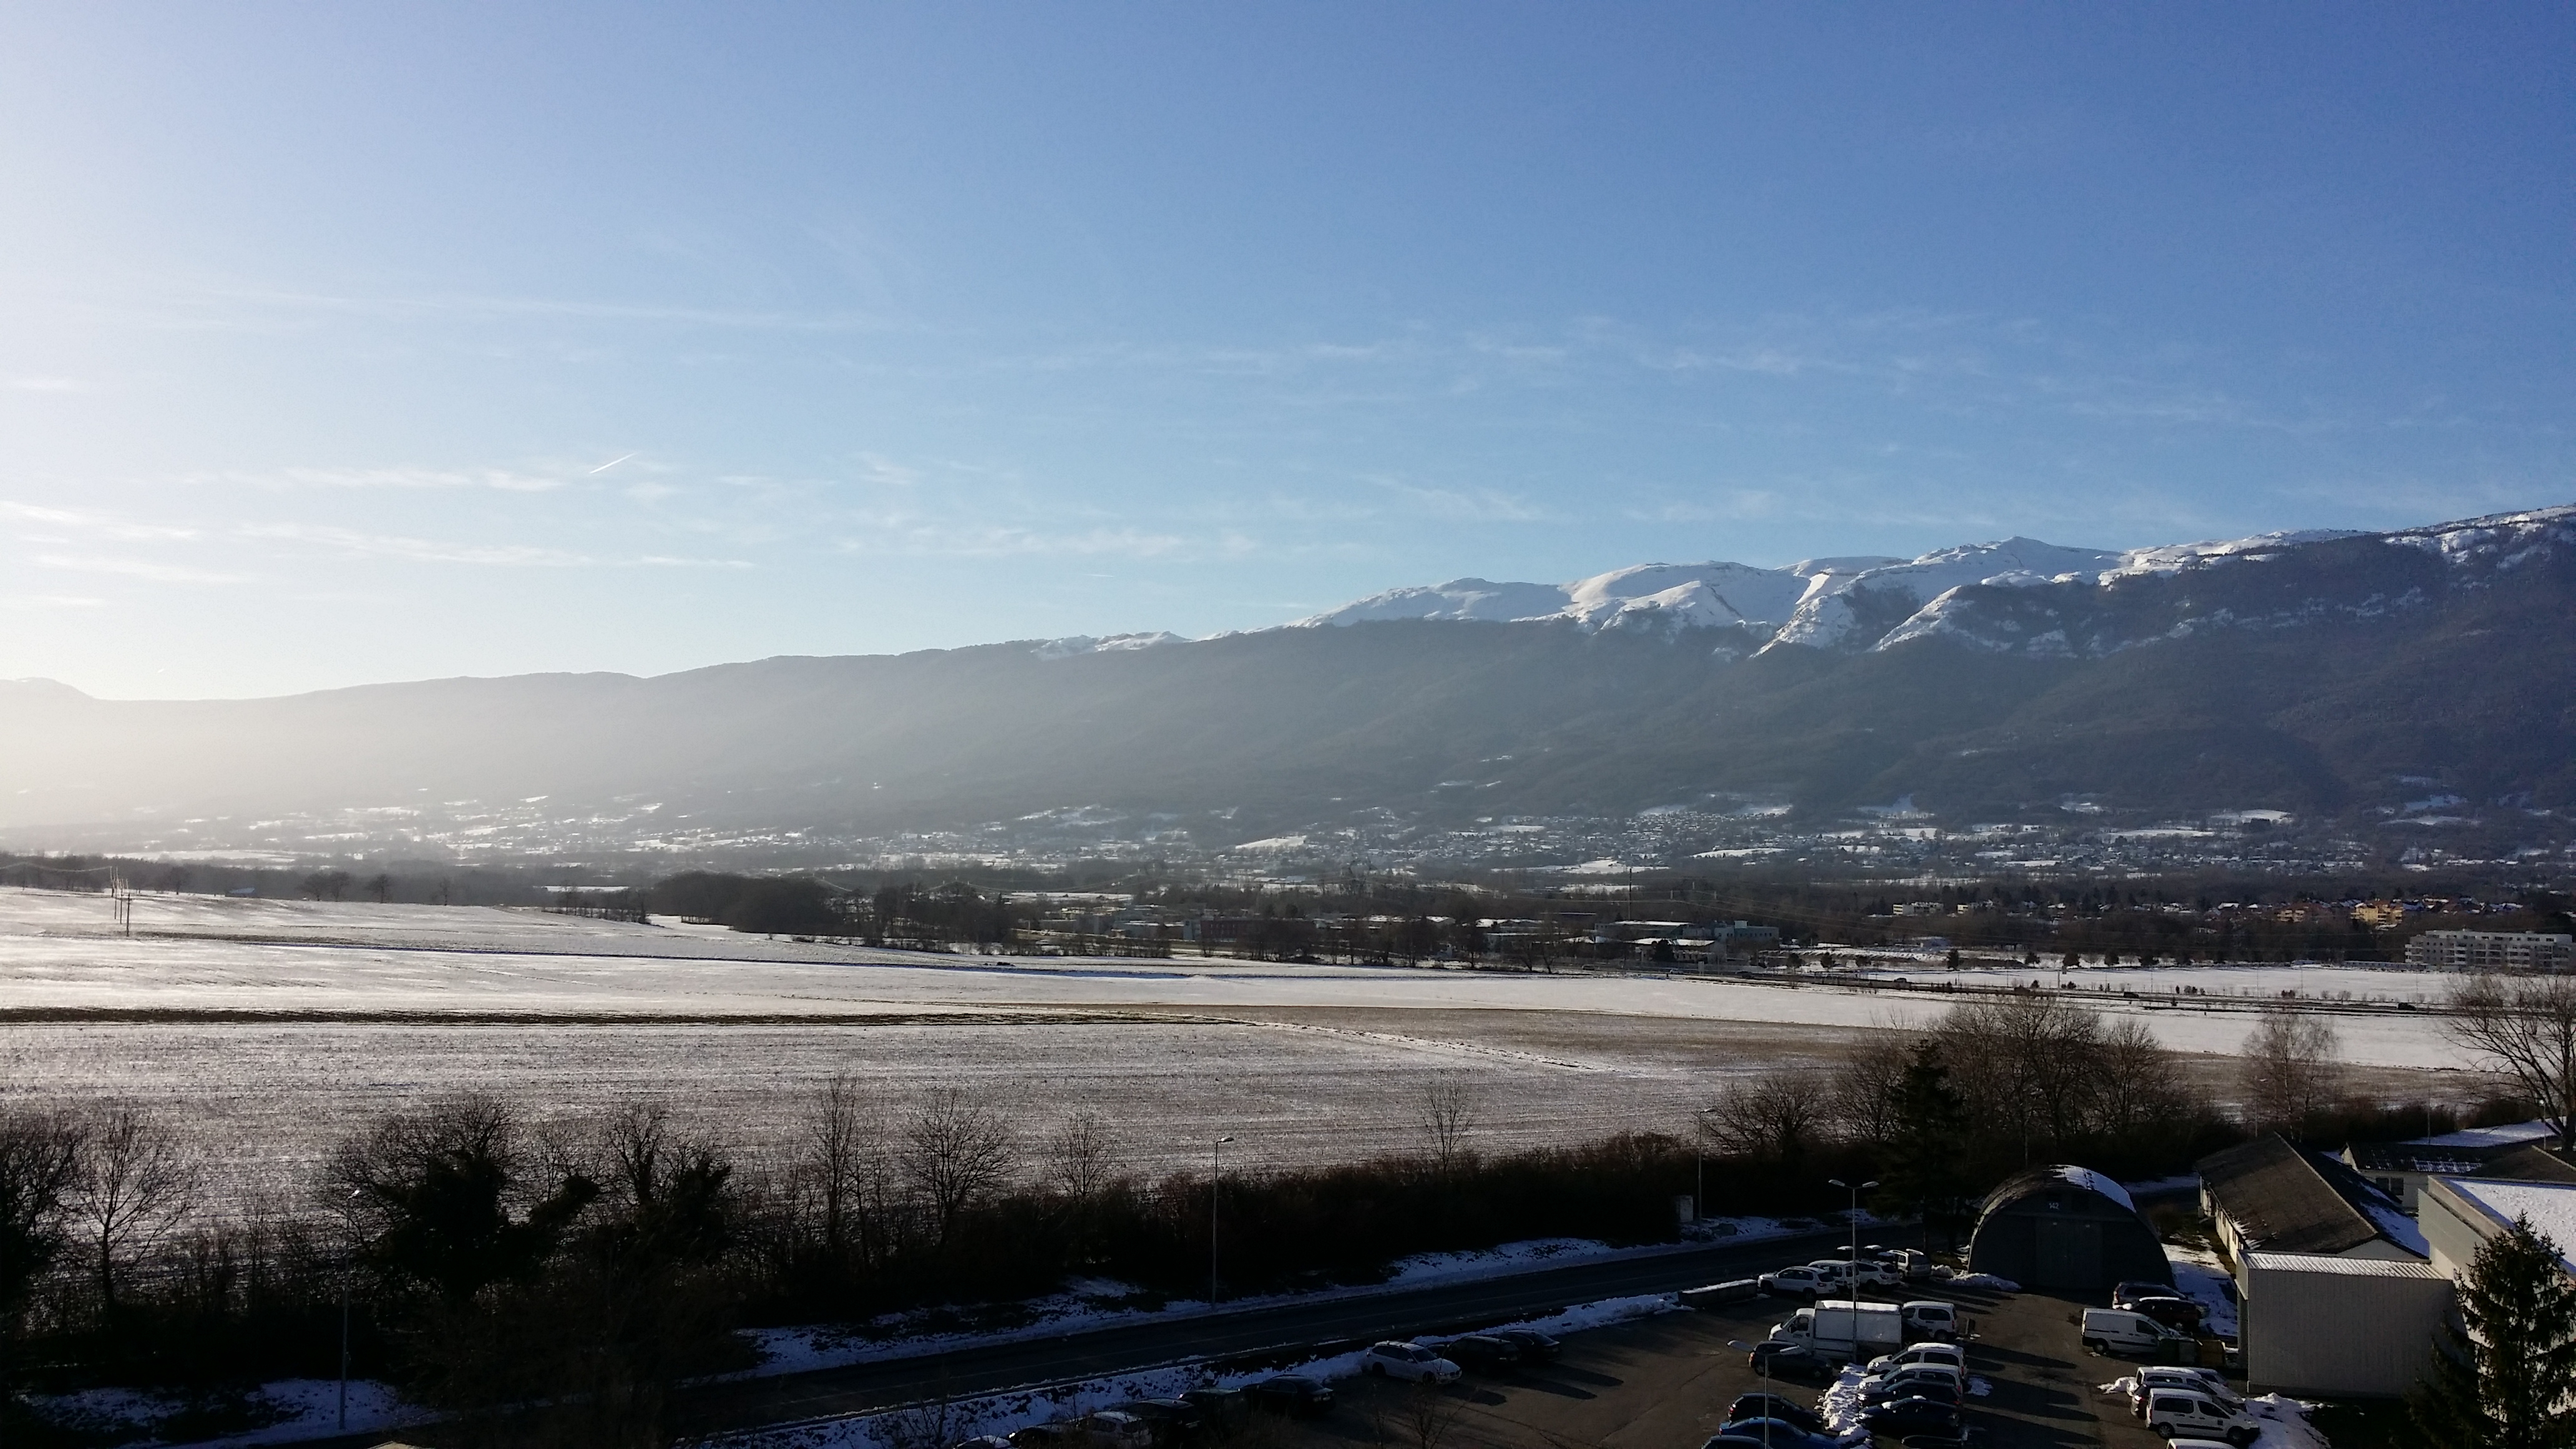
\includegraphics[width=\measureUSpecification]{images/2015-02-09T161202.jpg}\\
\end{center}
\end{frame}

\begin{frame}
\frametitle{an animated image (compatible with Adobe Reader)}
\vspace{-0.24 cm}
\begin{center}
%\animategraphics[
%    autoplay,
%    loop,
%    width=\measureUSpecification
%]{<frame rate>}{file path and basename}{<first>}{<last>}\\
\animategraphics[
    autoplay,
    loop,
    width=\measureUSpecification
]{30}{images/pool/pool_}{0}{29}\\
\end{center}
\end{frame}

\begin{frame}
\frametitle{a video (compatible with Okular)}
\vspace{-0.24 cm}
\begin{center}
\movie[
    height=6 cm,
    width=8 cm,
    showcontrols,
    poster
]{
\includegraphics[width=8 cm]{videos/hokeymon.png}}{videos/hokeymon.mp4}
\end{center}
\end{frame}

\begin{frame}
\frametitle{itemized list}
\begin{itemize}
\item item
\item item
    \begin{itemize}
    \item subitem
    \item subitem
        \begin{itemize}
        \item subitem
        \end{itemize}
    \end{itemize}
\item item
\item item
\end{itemize}
\end{frame}

\begin{frame}
\frametitle{enumerate list}
\begin{enumerate}
\item item
\item item
    \begin{enumerate}
    \item subitem
    \item subitem
        \begin{enumerate}
        \item subitem
        \end{enumerate}
    \end{enumerate}
\item item
\item item
\end{enumerate}
\end{frame}

\begin{frame}
\frametitle{description list}
\begin{description}
\item[A] item
\item[B] item
    \begin{description}
    \item[A] subitem
    \item[B] subitem
        \begin{description}
        \item[A] subitem
        \end{description}
    \end{description}
\item[C] item
\item[D] item
\end{description}
\end{frame}

% \checkmark (amsmath)
% \Checkmark
% \CheckmarkBold
% \XSolidBrush

\begin{frame}
\frametitle{description list with checkmarks}
\begin{description}
\item[\Checkmark] item
\item[\Checkmark] item
    \begin{description}
    \item[\Checkmark] subitem
    \item[\Checkmark] subitem
        \begin{description}
        \item[\Checkmark] subitem
        \end{description}
    \end{description}
\item[\Checkmark] item
\item[\XSolidBrush] item
\end{description}
\end{frame}

\begin{frame}
\frametitle{links}
\begin{itemize}
\item URL: \url{http://info.cern.ch/hypertext/WWW/TheProject.html}
\item hyperlink: \href{http://info.cern.ch/hypertext/WWW/TheProject.html}{TheProject}
\item hyperlink: \href{https://cds.cern.ch/record/1969527}{ATL-COM-PHYS-2014-1471}
\end{itemize}
\end{frame}

\begin{frame}
\frametitle{mathematics}
\begin{itemize}
\item ${H^{+}\to tb}$
\item lepton ${p_{T}}$ and ${\eta}$
\end{itemize}
\end{frame}

\begin{frame}
\frametitle{emoticons}
\begin{itemize}
\item smiley: \smiley
\item frownie: \frownie
\item neutralie: \neutralie
\end{itemize}
\end{frame}

\begin{frame}
\frametitle{centered text}
\begin{center}
some centered text\\\mbox{}\\some more centered text\\\mbox{}\\
\end{center}
\end{frame}

\begin{frame}
\frametitle{blocks}
\begin{block}{block 1}
\begin{itemize}
\item item
\item item
\end{itemize}
\end{block}
\begin{block}{block 2}
\begin{itemize}
\item item
\item item
\end{itemize}
\end{block}
\end{frame}

\begin{frame}
\frametitle{columns (2)}
\begin{columns}
\begin{column}[t]{.5\textwidth}
\justifying
Lorem ipsum dolor sit amet, consectetuer adipiscing elit. Aenean commodo ligula eget dolor. Aenean massa. Cum sociis natoque penatibus et magnis dis parturient montes, nascetur ridiculus mus. Donec quam felis, ultricies nec, pellentesque eu, pretium quis, sem.
\end{column}
\hfill
\begin{column}[t]{.5\textwidth}
\justifying
Nulla consequat massa quis enim. Donec pede justo, fringilla vel, aliquet nec, vulputate eget, arcu. In enim justo, rhoncus ut, imperdiet a, venenatis vitae, justo. Nullam dictum felis eu pede mollis pretium.
\end{column}%
\end{columns}
\end{frame}

\begin{frame}
\frametitle{multiple columns (2)}
\setlength\columnsep{30pt}
\begin{multicols}{2}
\justifying
Lorem ipsum dolor sit amet, consectetuer adipiscing elit. Aenean commodo ligula eget dolor. Aenean massa. Cum sociis natoque penatibus et magnis dis parturient montes, nascetur ridiculus mus. Donec quam felis, ultricies nec, pellentesque eu, pretium quis, sem. Nulla consequat massa quis enim. Donec pede justo, fringilla vel, aliquet nec, vulputate eget, arcu. In enim justo, rhoncus ut, imperdiet a, venenatis vitae, justo. Nullam dictum felis eu pede mollis pretium.
\end{multicols}
\end{frame}

\begin{frame}
\frametitle{multiple columns (4)}
\setlength\columnsep{30pt}
\begin{multicols}{4}
\justifying
Lorem ipsum dolor sit amet, consectetuer adipiscing elit. Aenean commodo ligula eget dolor. Aenean massa. Cum sociis natoque penatibus et magnis dis parturient montes, nascetur ridiculus mus. Donec quam felis, ultricies nec, pellentesque eu, pretium quis, sem. Nulla consequat massa quis enim. Donec pede justo, fringilla vel, aliquet nec, vulputate eget, arcu. In enim justo, rhoncus ut, imperdiet a, venenatis vitae, justo. Nullam dictum felis eu pede mollis pretium.
\end{multicols}
\end{frame}

%\begin{frame}[fragile]
%\frametitle{global interpreter lock (GIL) in Python}
%The Python interpreter is not fully thread safe and, so, a GIL is implemented in order to support multithreaded Python programs. Without the GIL, even many simple operations are problematic (e.g. incrementing the reference count of some common object simultaneously in two threads could result in a single increment, rather than the intended two increments).\\
%\mbox{}\\
%rule: Only the thread that has acquired the GIL my operate on Python objects or call API functions.\\
%\mbox{}\\
%The Python interpreter attempts to switch threads regularly (using \pythoninline{set.checkinterval()}) in order to emulate concurrency.
%\end{frame}

%\begin{frame}[fragile]
%\frametitle{a taste of Python multiprocessing: creating a process}
%\begin{python}
%from multiprocessing import Process
%
%def function1(text):
%    print(text)
%
%if __name__ == "__main__":
%    process1 = Process(target = function1, args = ("hello world",))
%    process1.start()
%    process1.join()
%\end{python}
%\end{frame}

\begin{frame}
\frametitle{${8\textrm{ TeV}}$ vs.~${13\textrm{ TeV}}$: cutflow for ${l+\textrm{jets}}$}
\begin{center}
\begin{tabular}{cc}
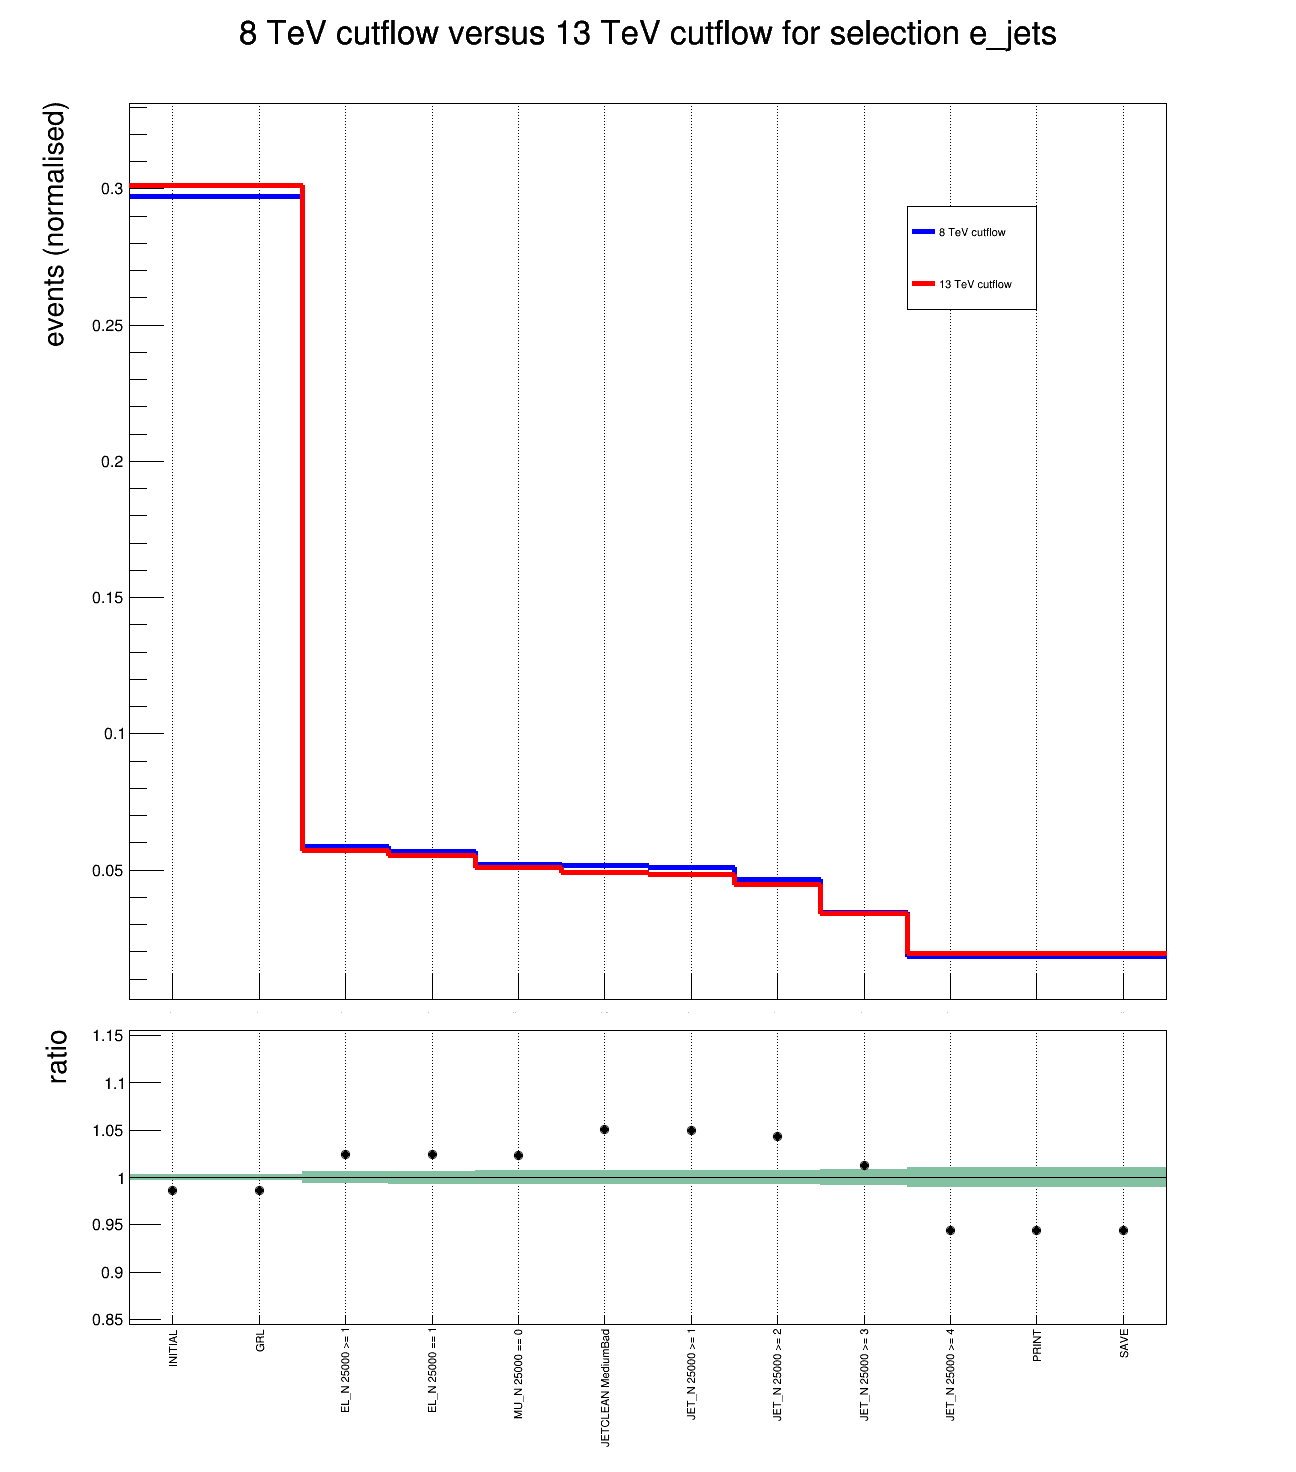
\includegraphics[width=\measureNSpecification]{images_2/2015-04-21T0410Z_cutflow_e_jets.png}&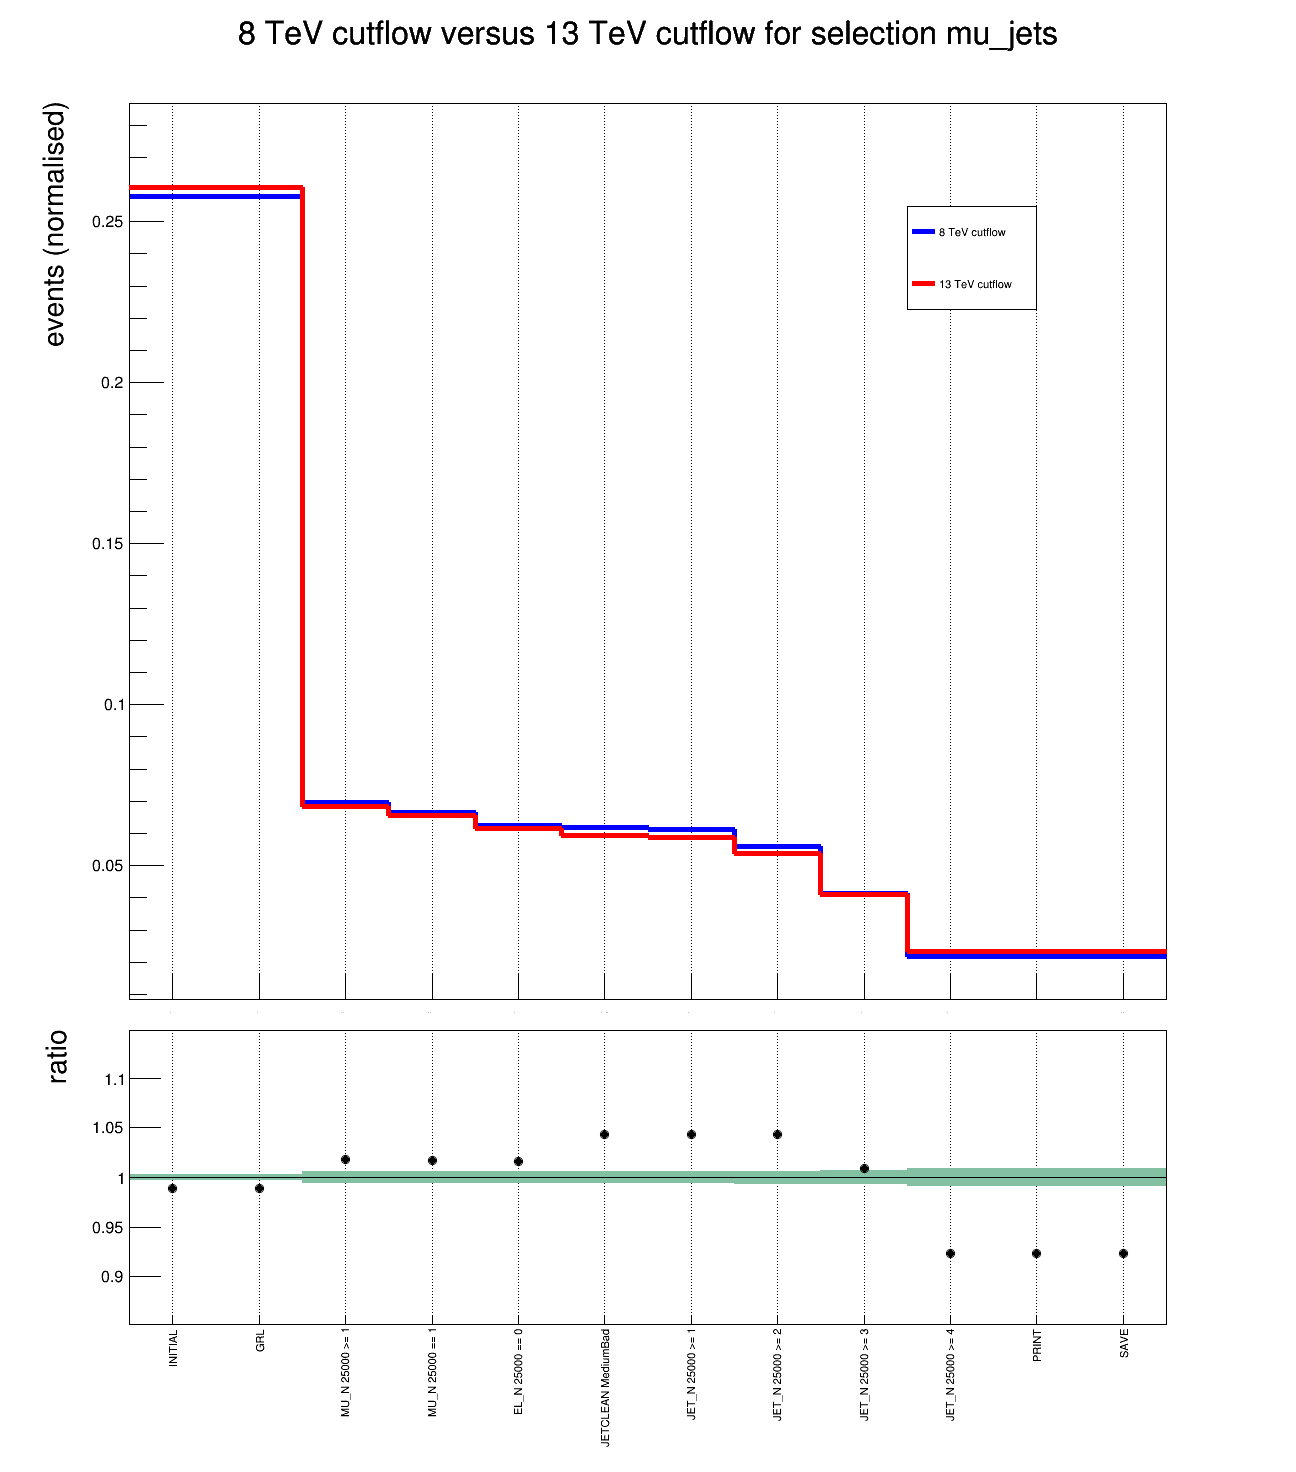
\includegraphics[width=\measureNSpecification]{images_2/2015-04-21T0410Z_cutflow_mu_jets.png}\\
\end{tabular}
\end{center}
\end{frame}

\begin{frame}
\frametitle{${8\textrm{ TeV}}$ vs.~${13\textrm{ TeV}}$: cutflow for dilepton}
\begin{center}
\begin{tabular}{ccc}
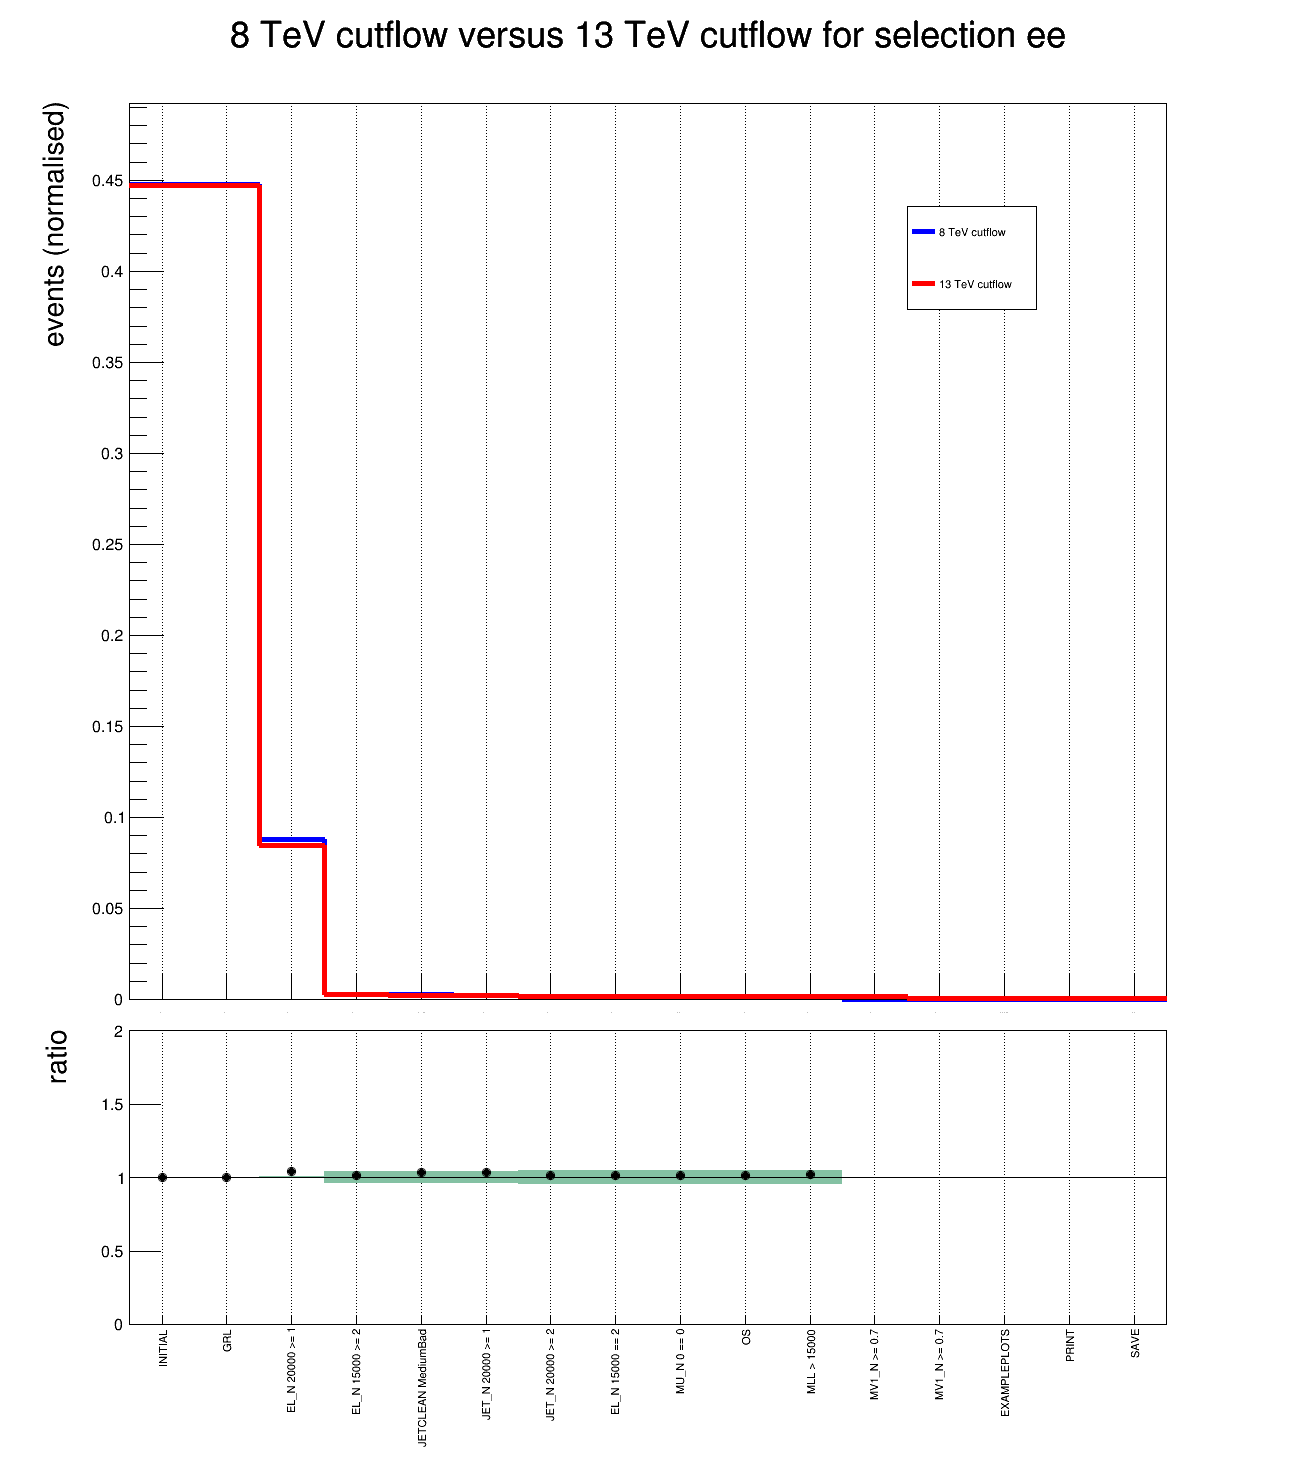
\includegraphics[width=\measureMSpecification]{images_2/2015-04-21T0410Z_cutflow_ee.png}&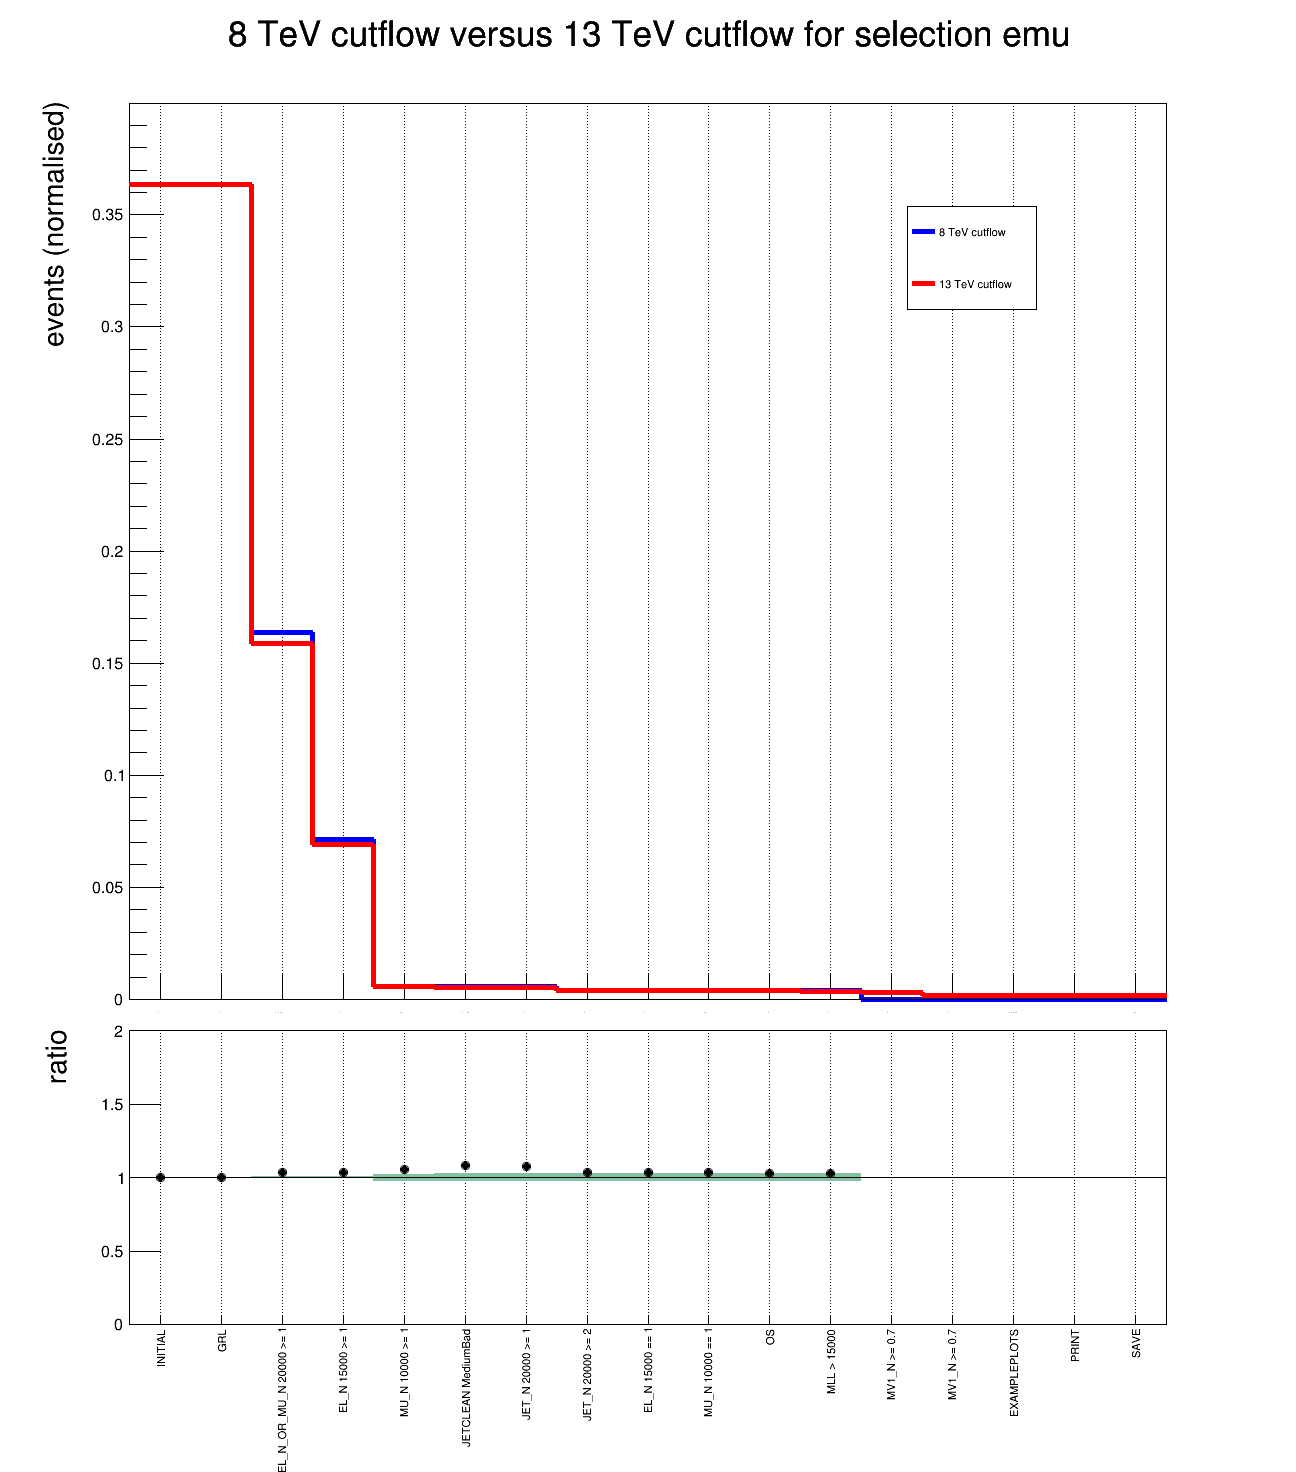
\includegraphics[width=\measureMSpecification]{images_2/2015-04-21T0410Z_cutflow_emu.png}&
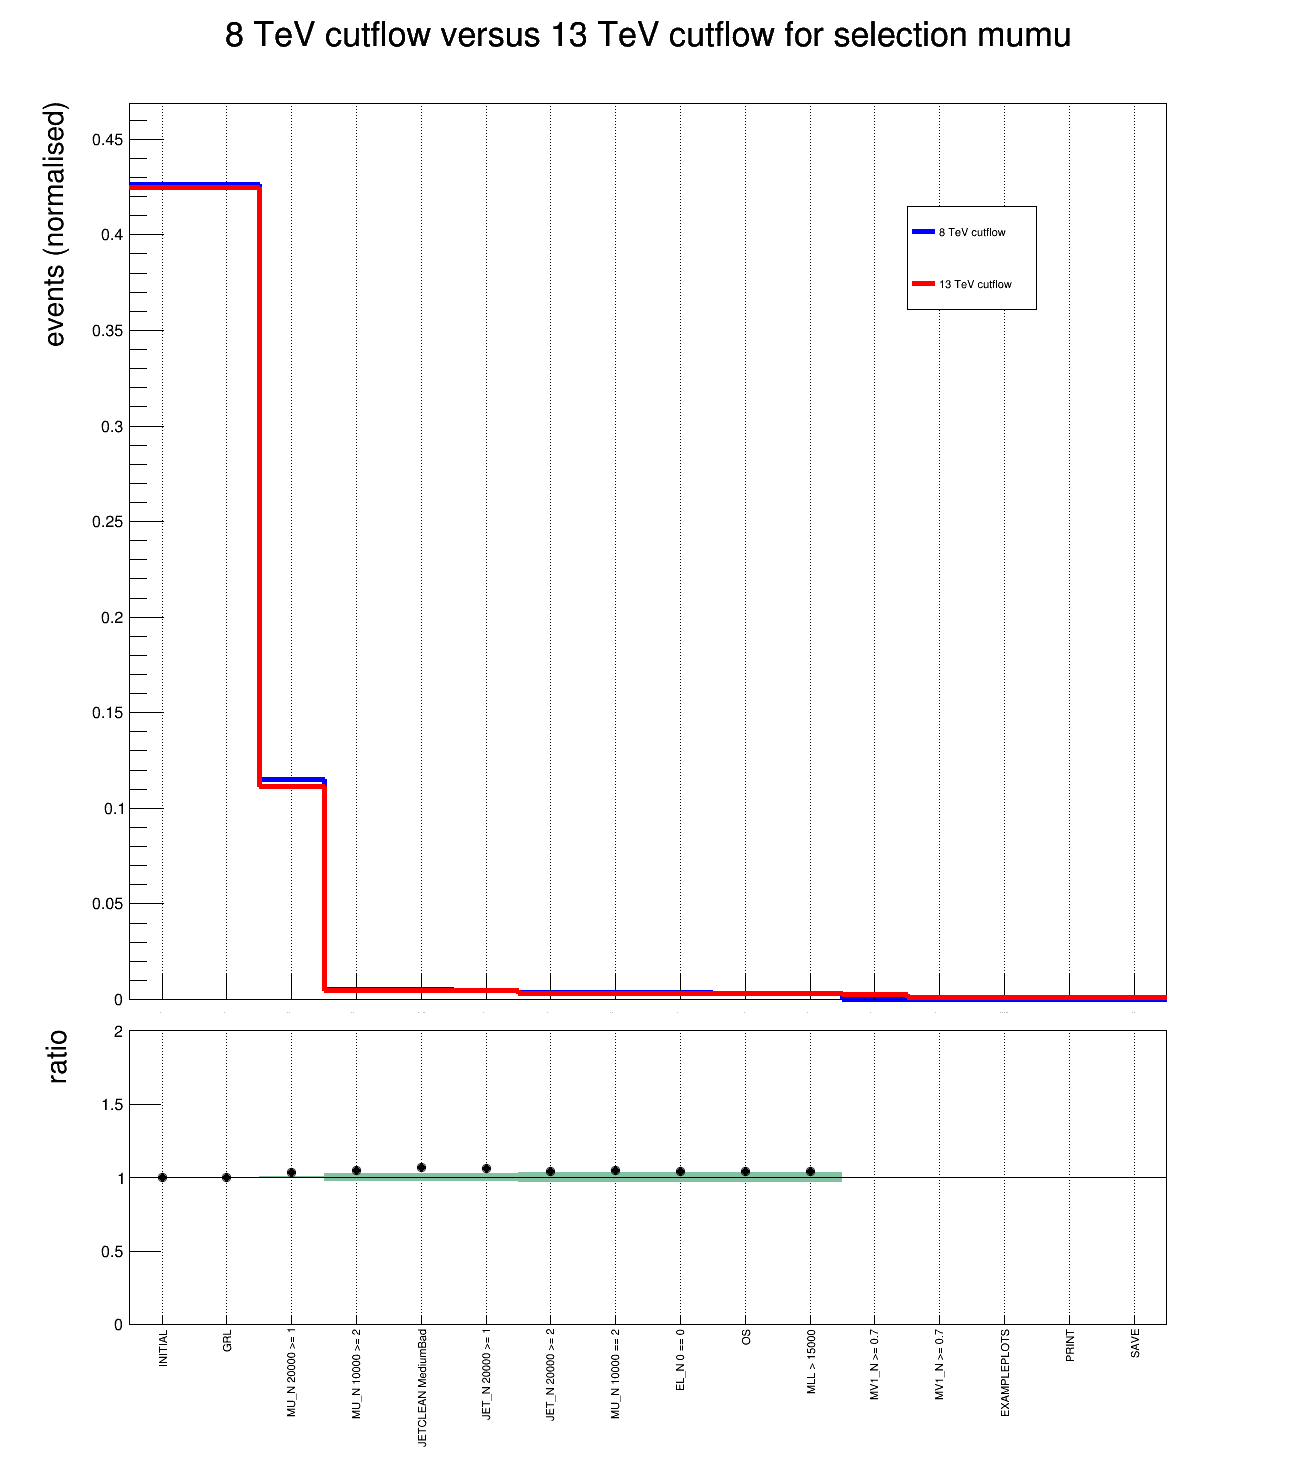
\includegraphics[width=\measureMSpecification]{images_2/2015-04-21T0410Z_cutflow_mumu.png}\\
\end{tabular}
\vspace{0.5 cm}\\I3PD+SV1: \url{https://indico.cern.ch/event/387410/contribution/9/material/slides/0.pdf}
\end{center}
\end{frame}

\begin{frame}
\frametitle{${8\textrm{ TeV}}$ vs.~${13\textrm{ TeV}}$: centrality}
\begin{center}
\begin{tabular}{cc}
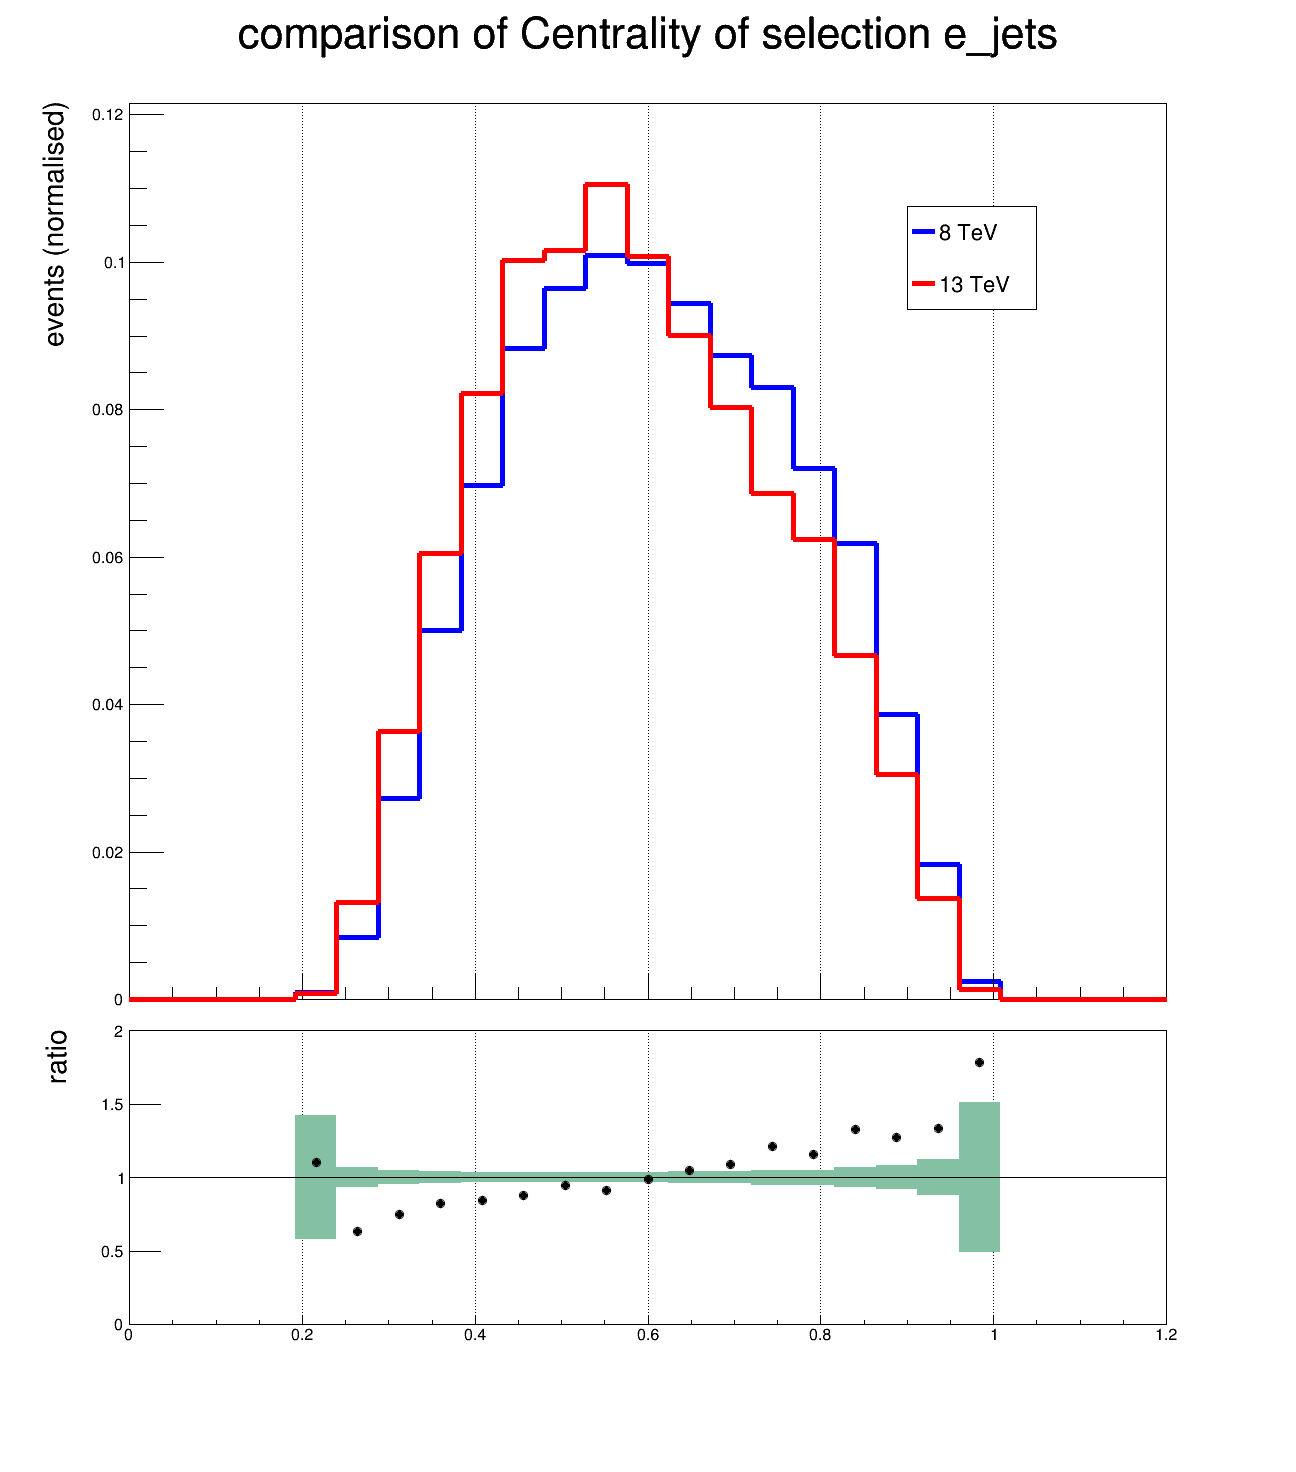
\includegraphics[width=\measureNSpecification]{images_2/2015-04-21T0410Z_comparison_of_Centrality_of_selection_e_jets.png}&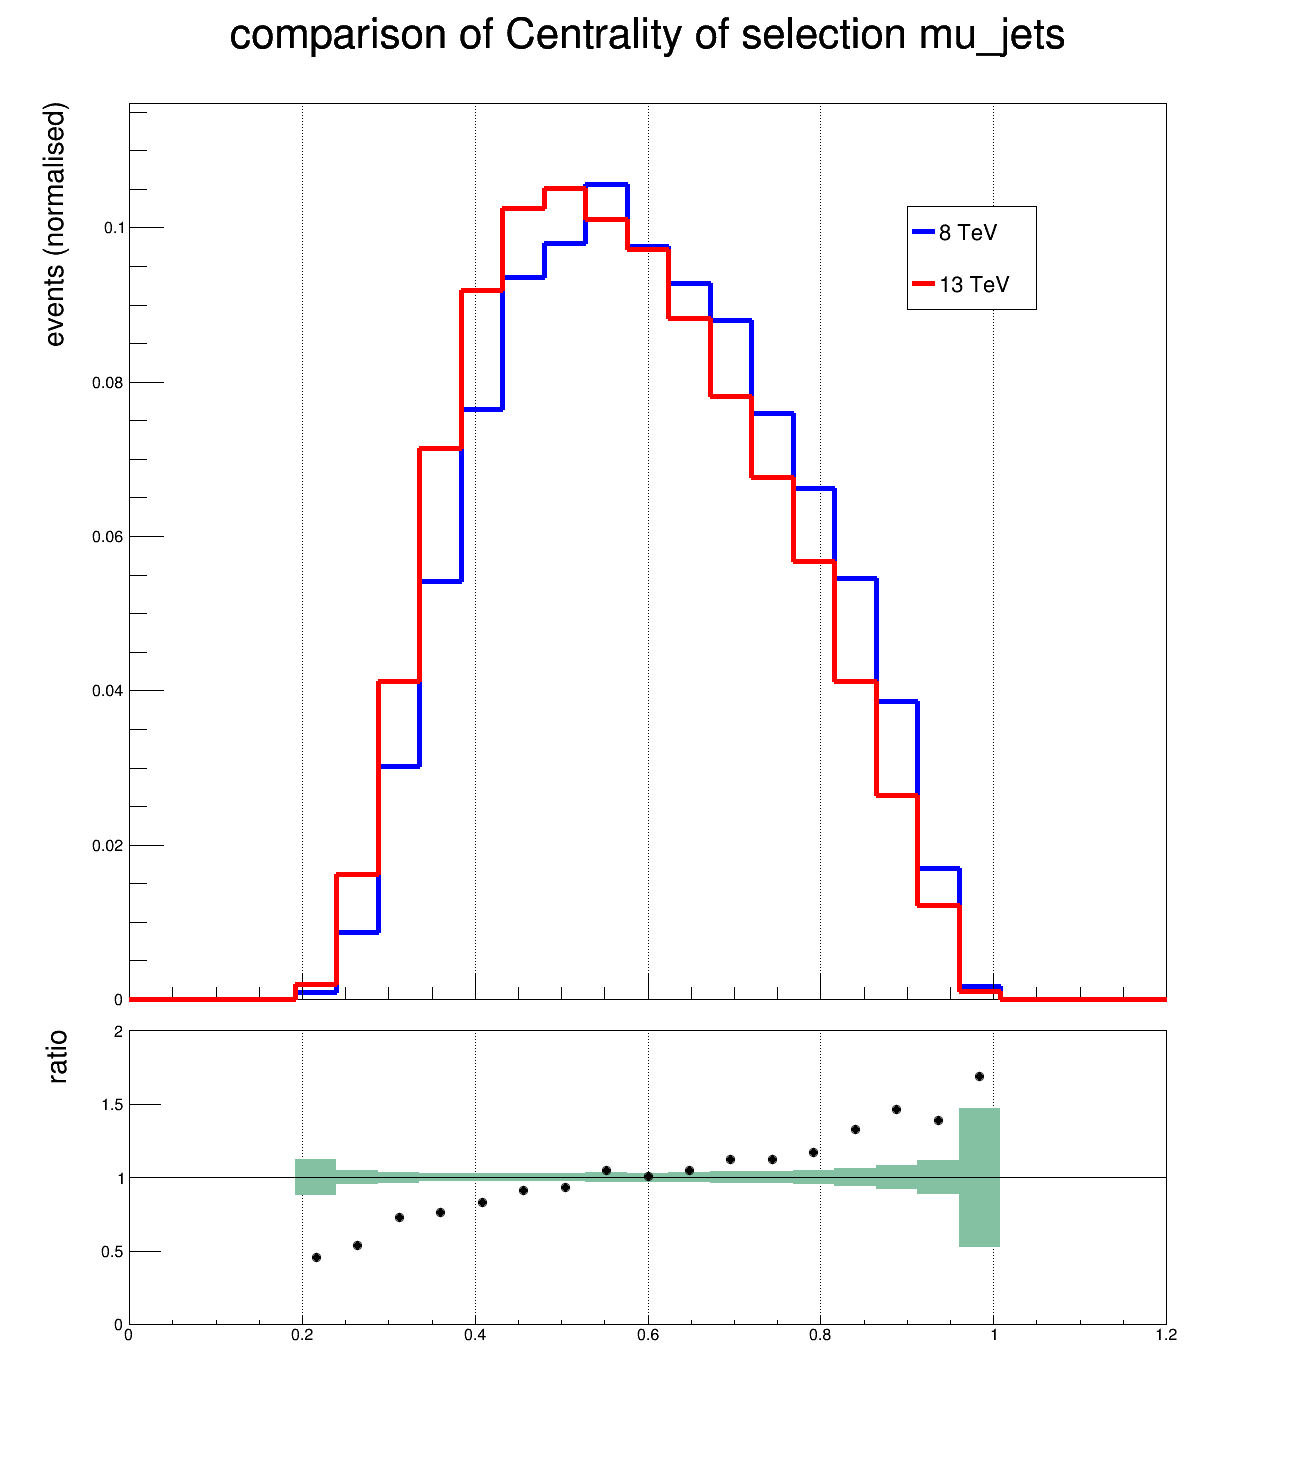
\includegraphics[width=\measureNSpecification]{images_2/2015-04-21T0410Z_comparison_of_Centrality_of_selection_mu_jets.png}\\
\end{tabular}
\end{center}
\end{frame}

\begin{frame}
\frametitle{${8\textrm{ TeV}}$ vs.~${13\textrm{ TeV}}$: JVF}
\begin{center}
\begin{tabular}{cc}
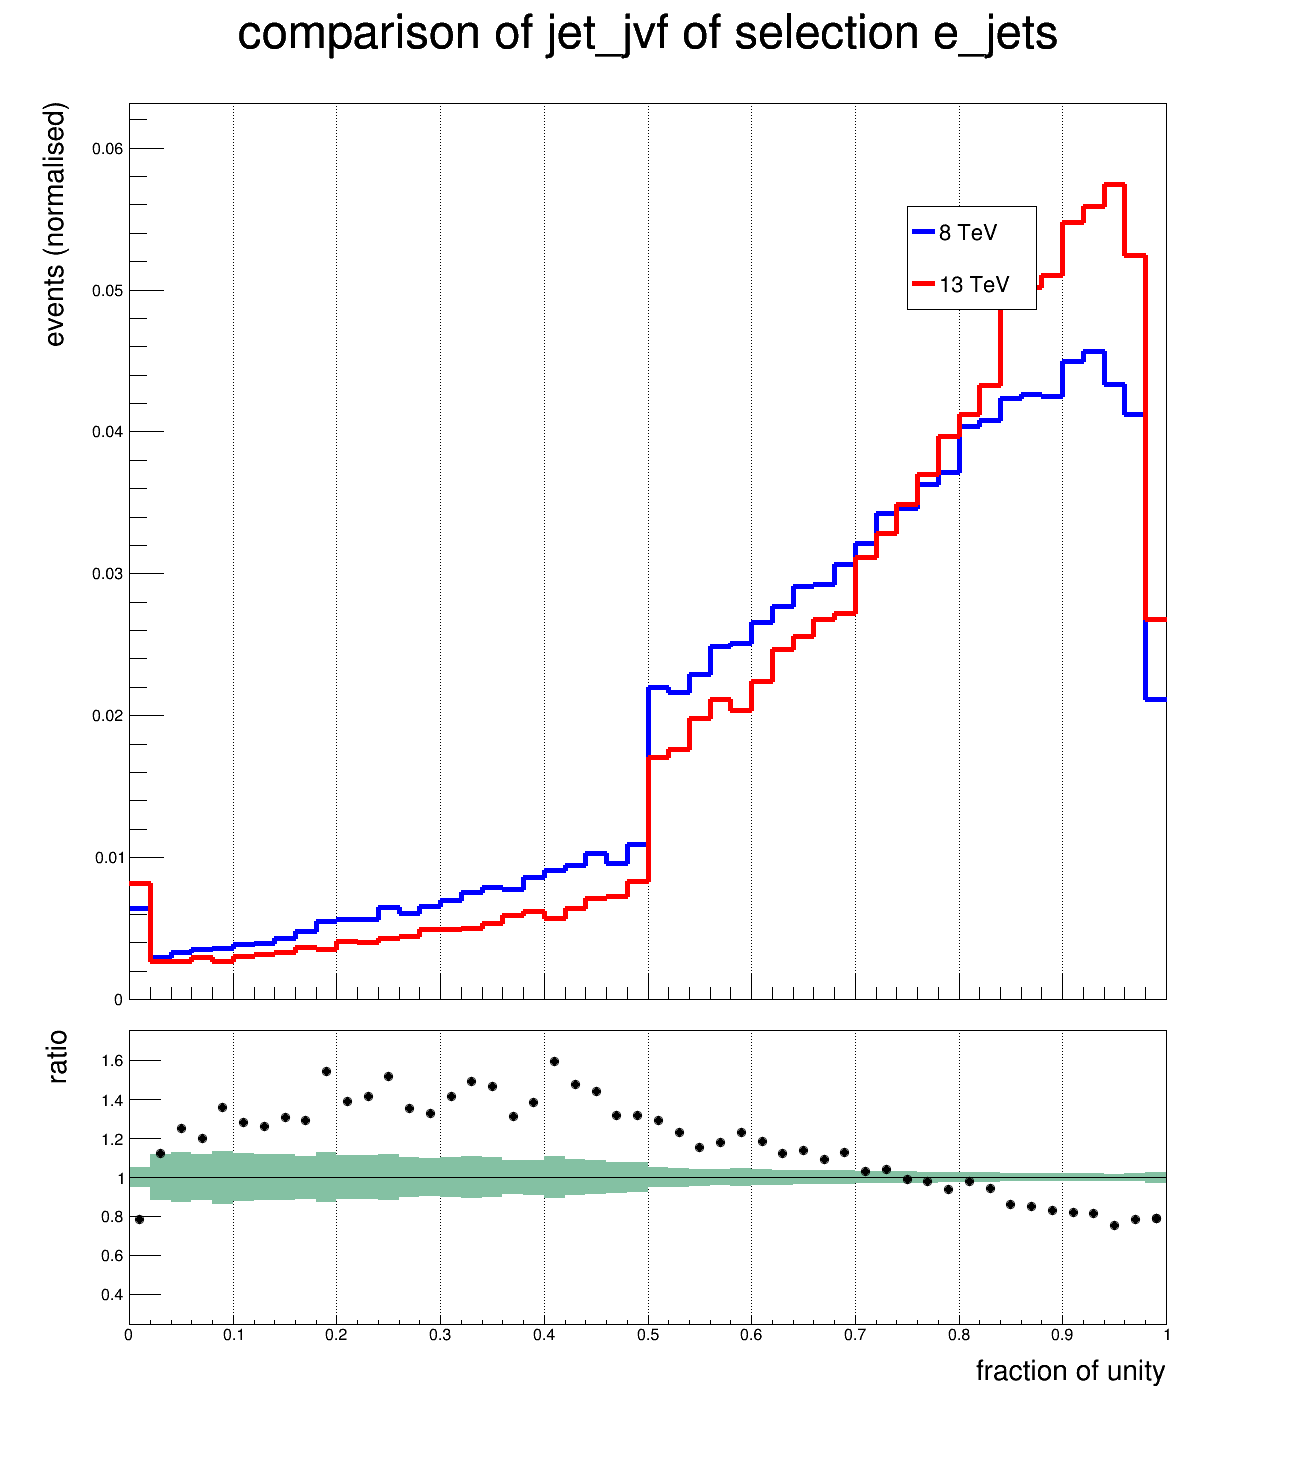
\includegraphics[width=\measureNSpecification]{images_2/2015-04-21T0410Z_comparison_of_jet_jvf_of_selection_e_jets.png}&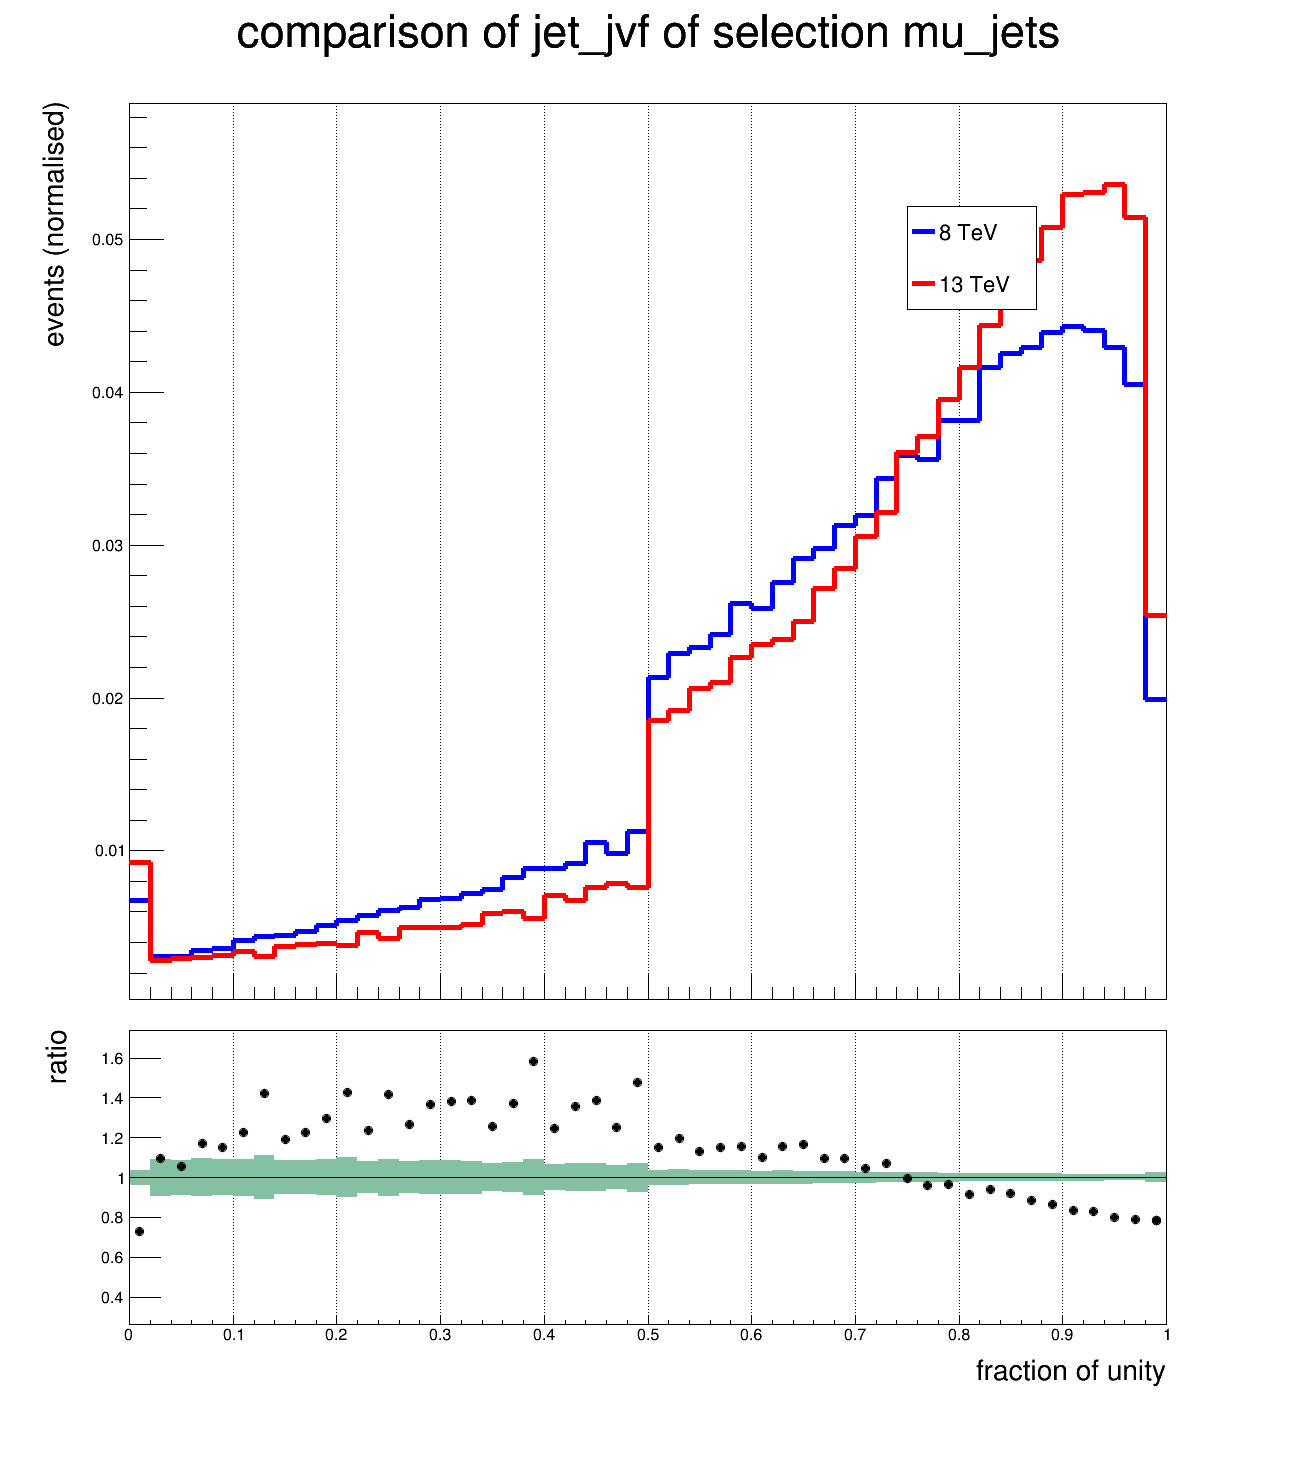
\includegraphics[width=\measureNSpecification]{images_2/2015-04-21T0410Z_comparison_of_jet_jvf_of_selection_mu_jets.png}\\
\end{tabular}
\end{center}
\end{frame}

\begin{frame}
\frametitle{${8\textrm{ TeV}}$ vs.~${13\textrm{ TeV}}$: subleading jets ${p_{T}}$ of ${e}$ selection}
\begin{center}
\begin{tabular}{ccc}
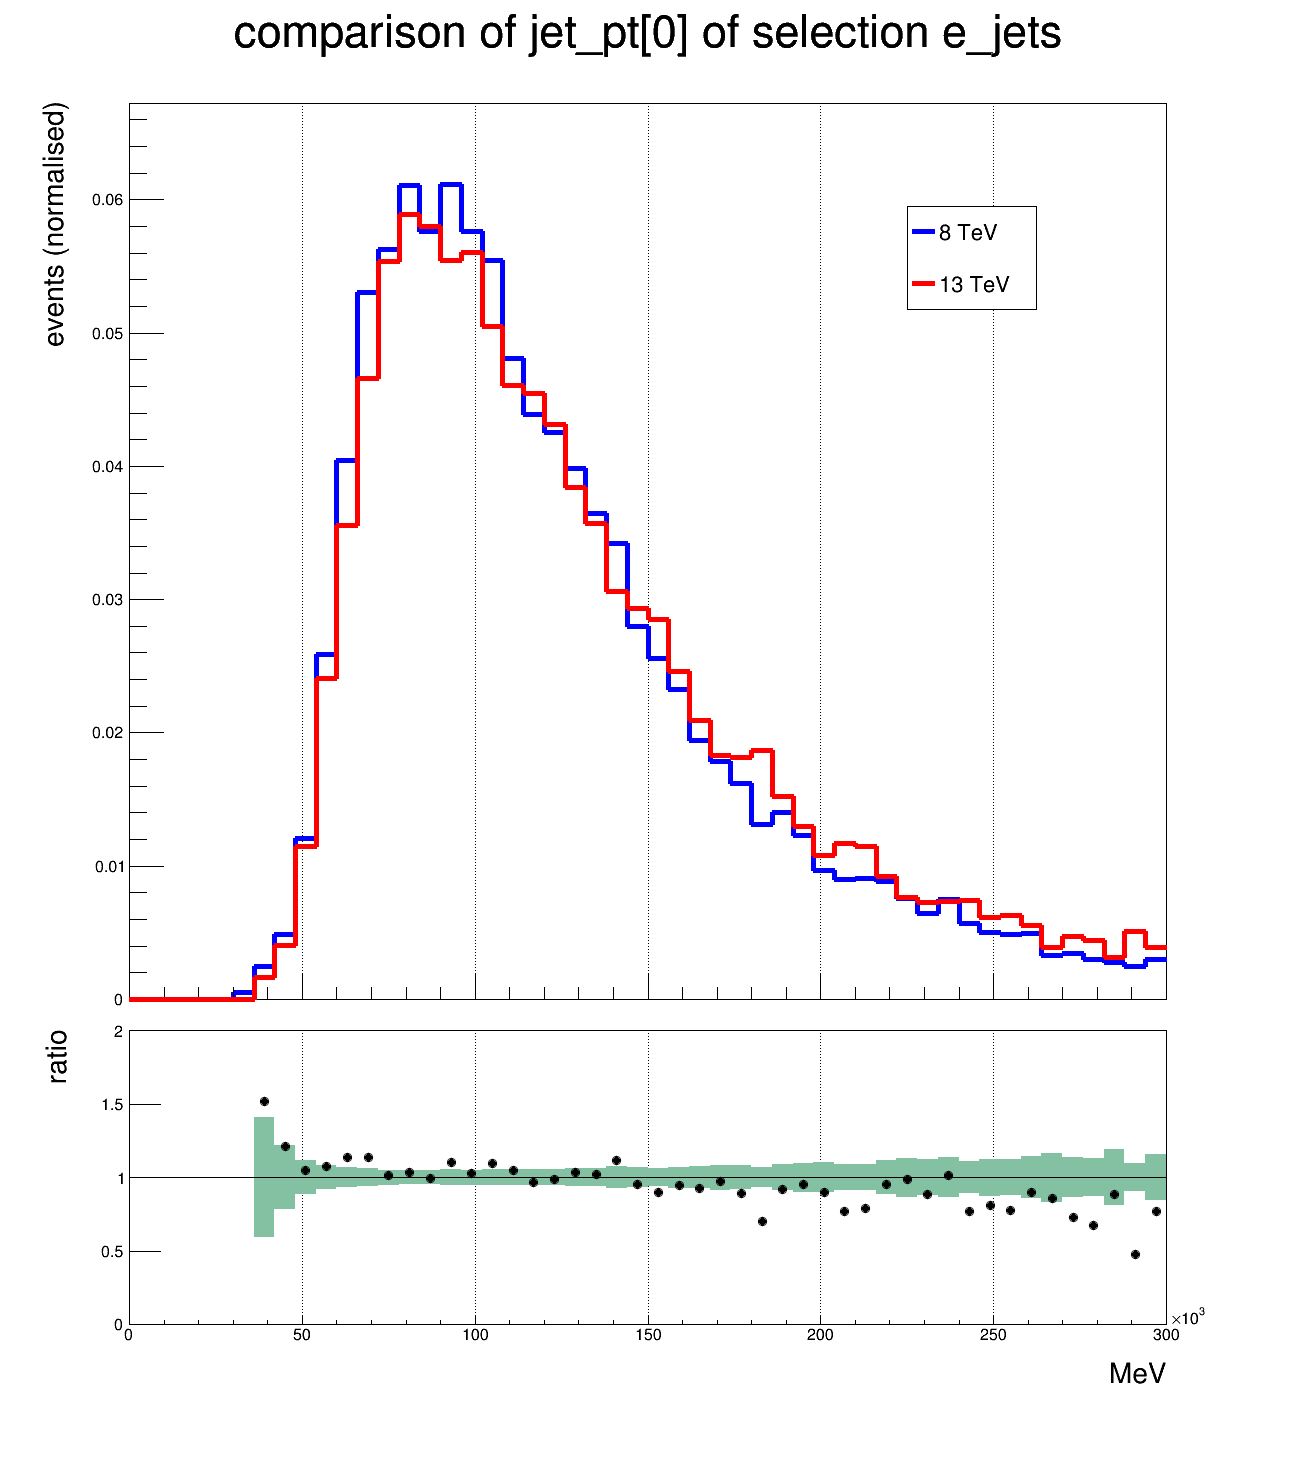
\includegraphics[width=\measureLSpecification]{images_2/2015-04-21T0410Z_comparison_of_jet_pt[0]_of_selection_e_jets.png}&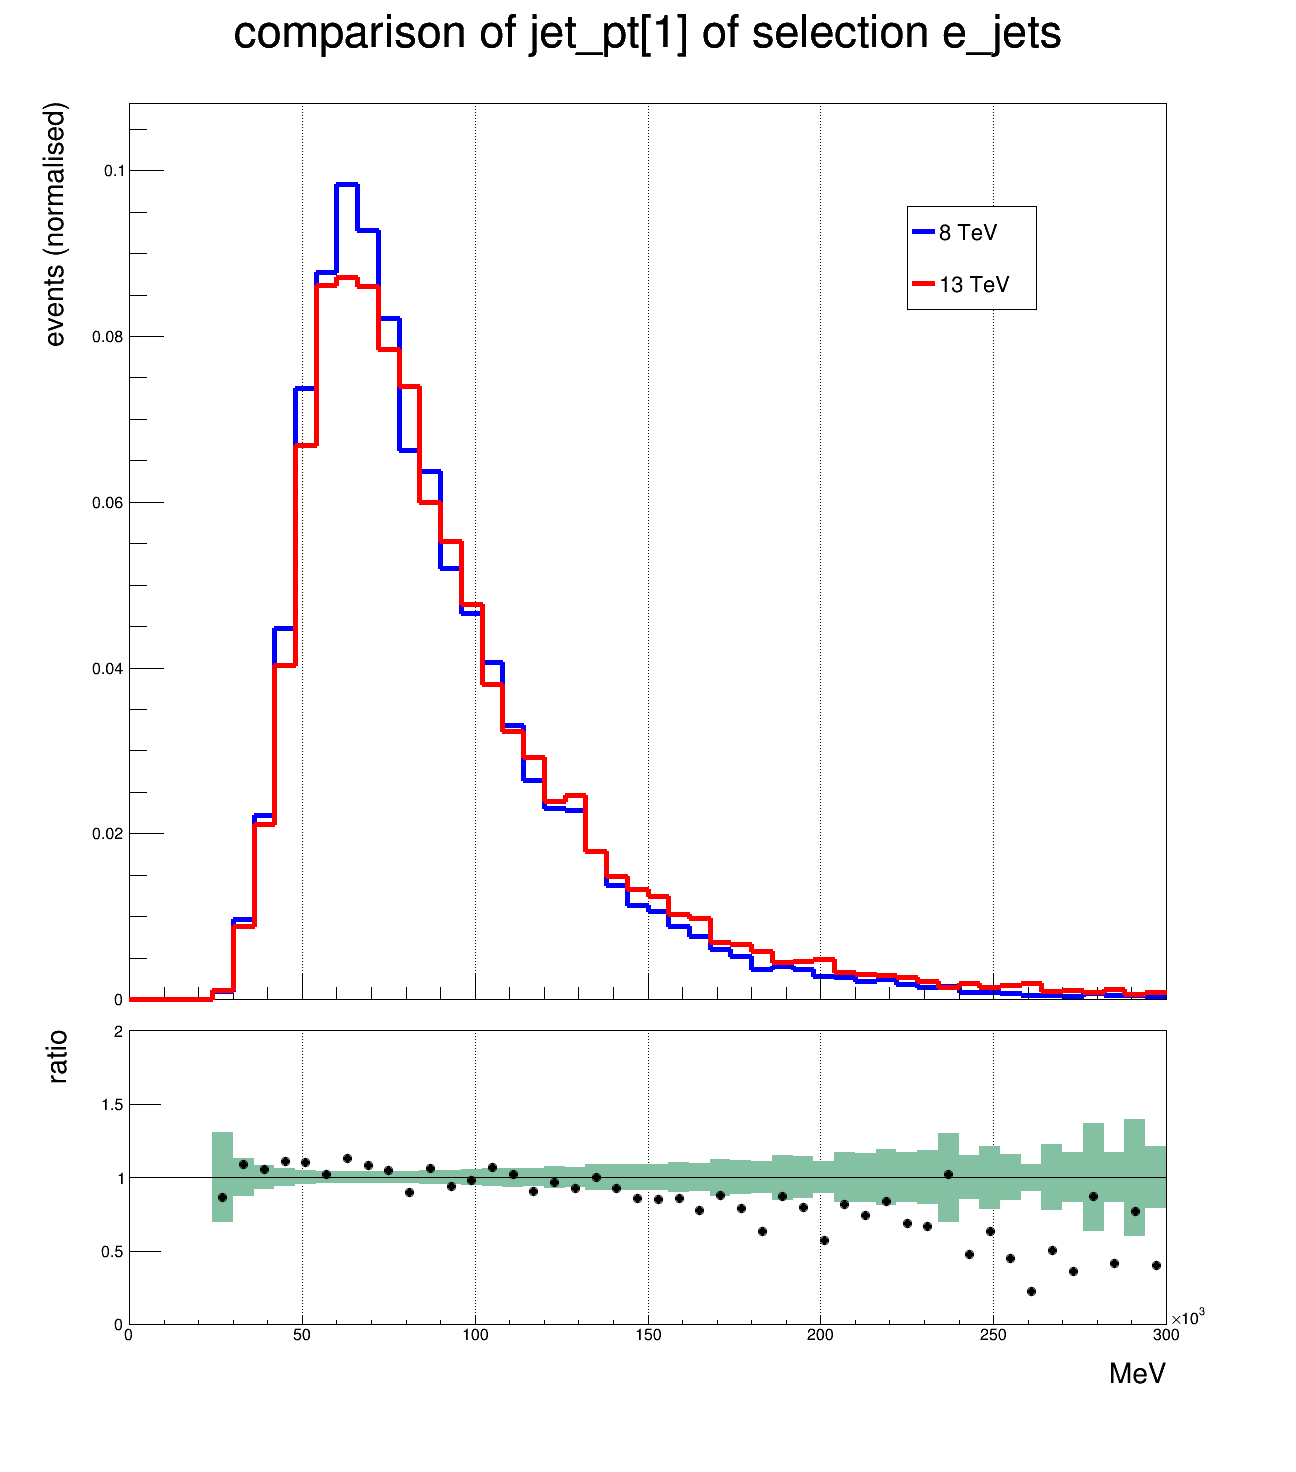
\includegraphics[width=\measureLSpecification]{images_2/2015-04-21T0410Z_comparison_of_jet_pt[1]_of_selection_e_jets.png}&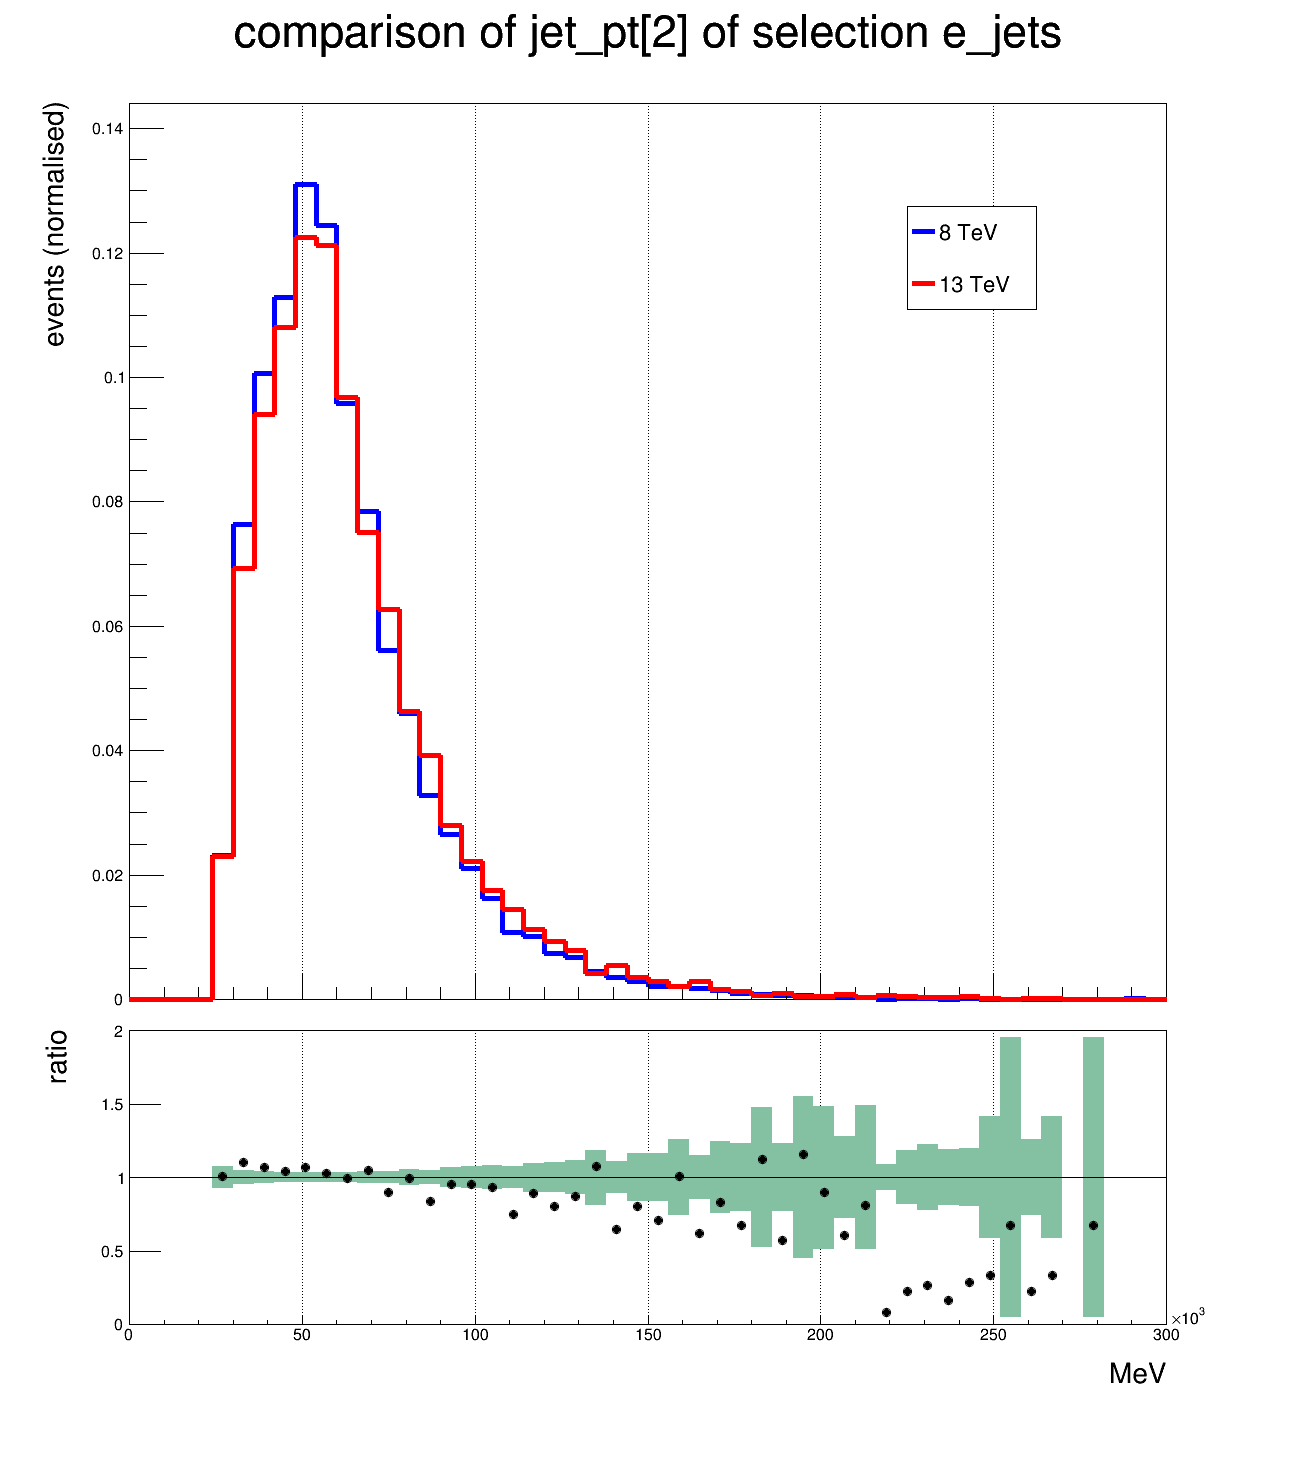
\includegraphics[width=\measureLSpecification]{images_2/2015-04-21T0410Z_comparison_of_jet_pt[2]_of_selection_e_jets.png}\\
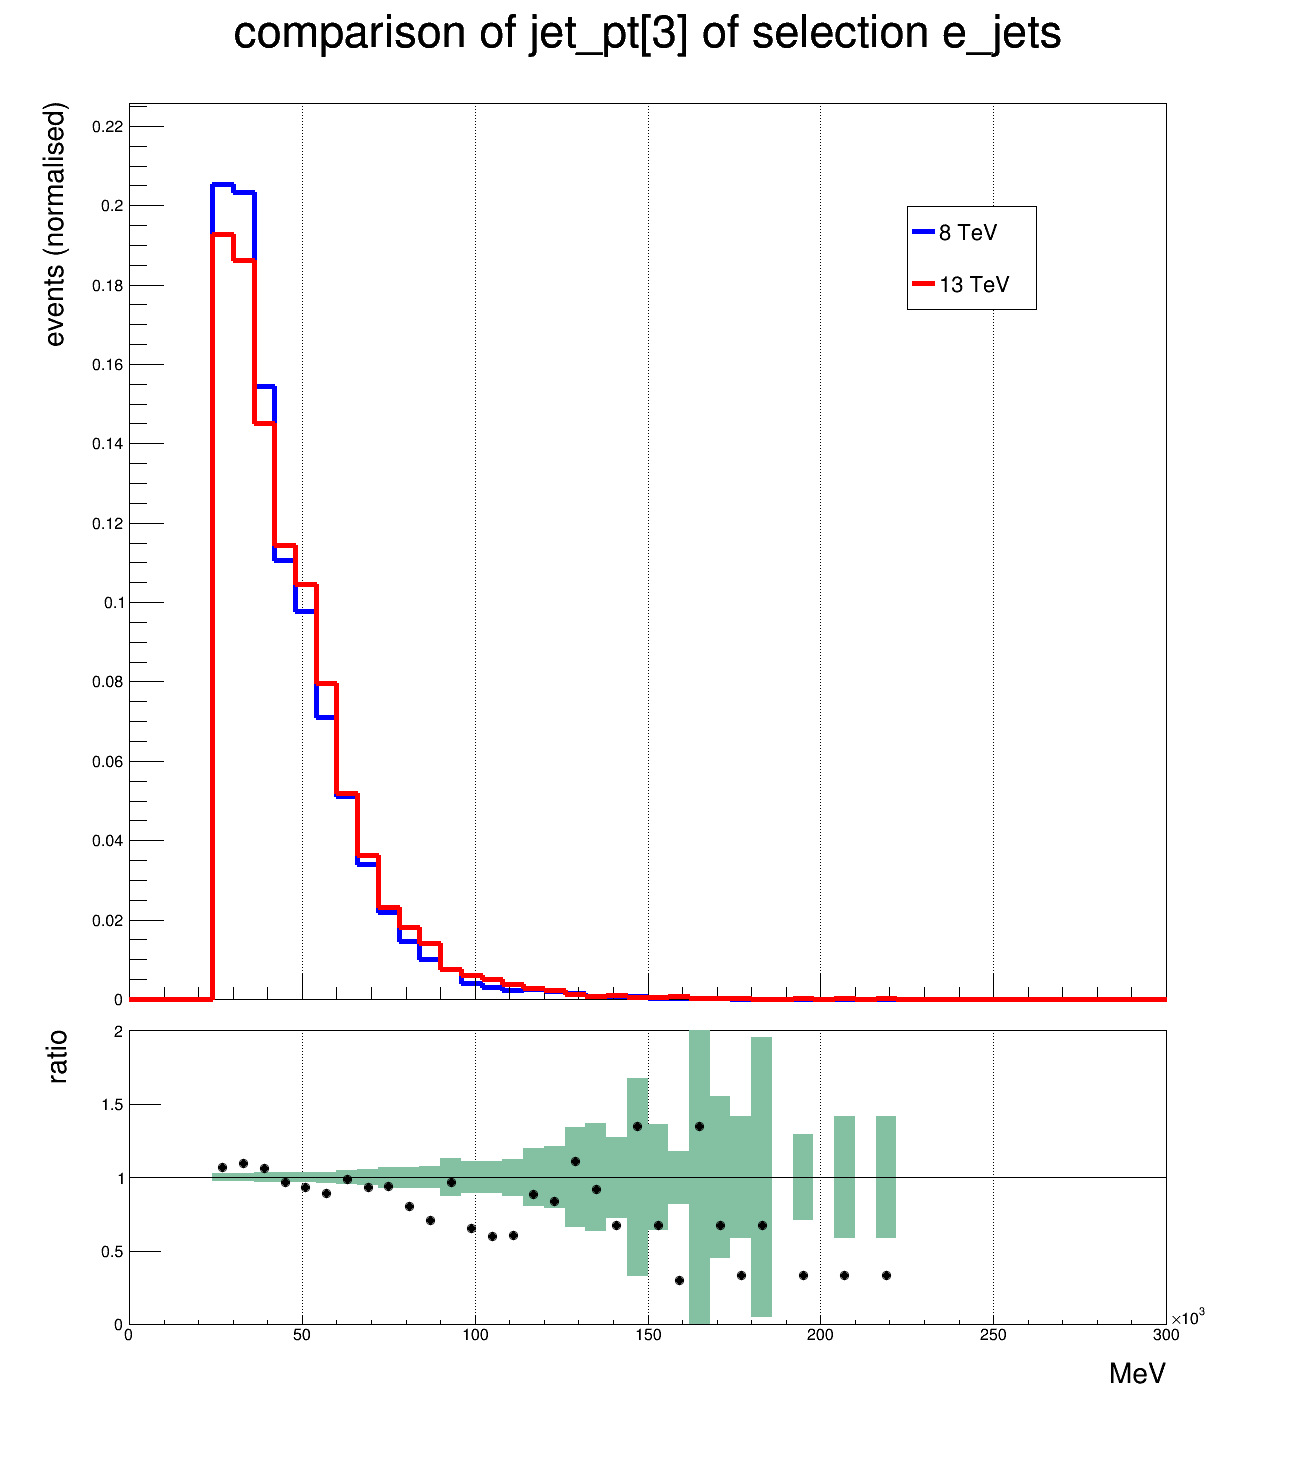
\includegraphics[width=\measureLSpecification]{images_2/2015-04-21T0410Z_comparison_of_jet_pt[3]_of_selection_e_jets.png}&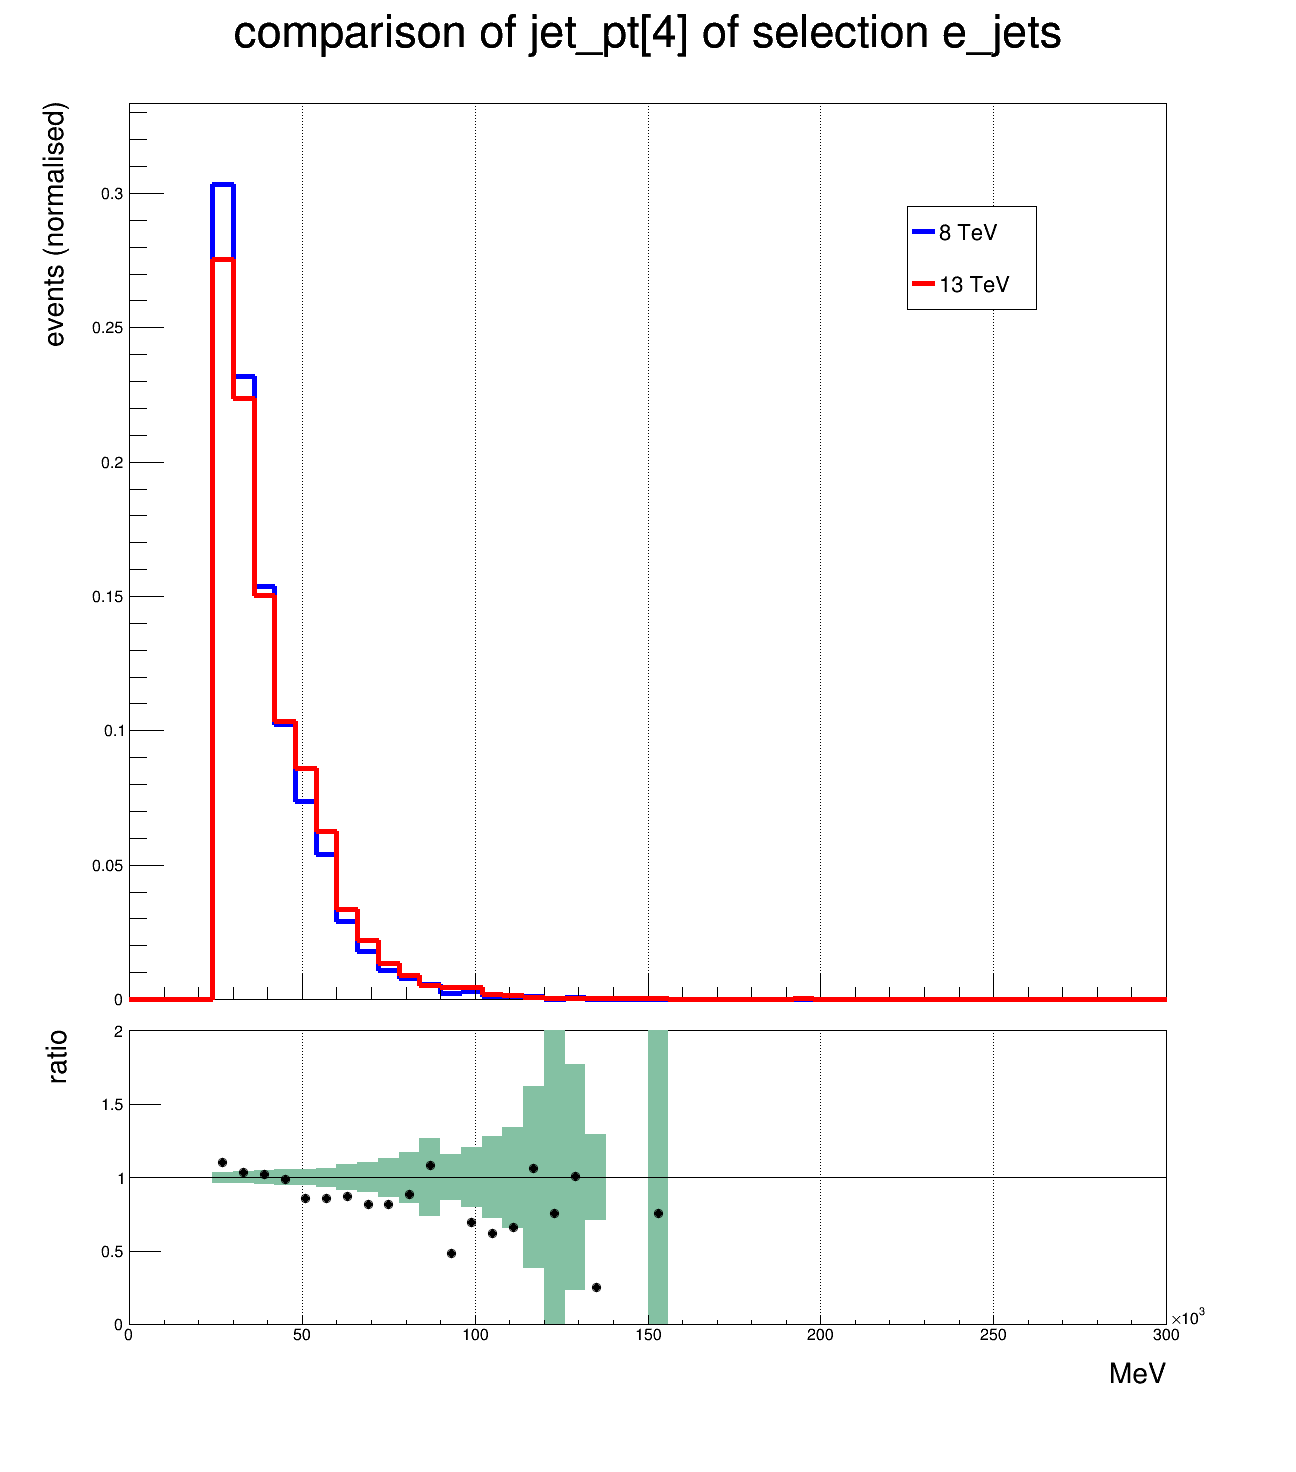
\includegraphics[width=\measureLSpecification]{images_2/2015-04-21T0410Z_comparison_of_jet_pt[4]_of_selection_e_jets.png}&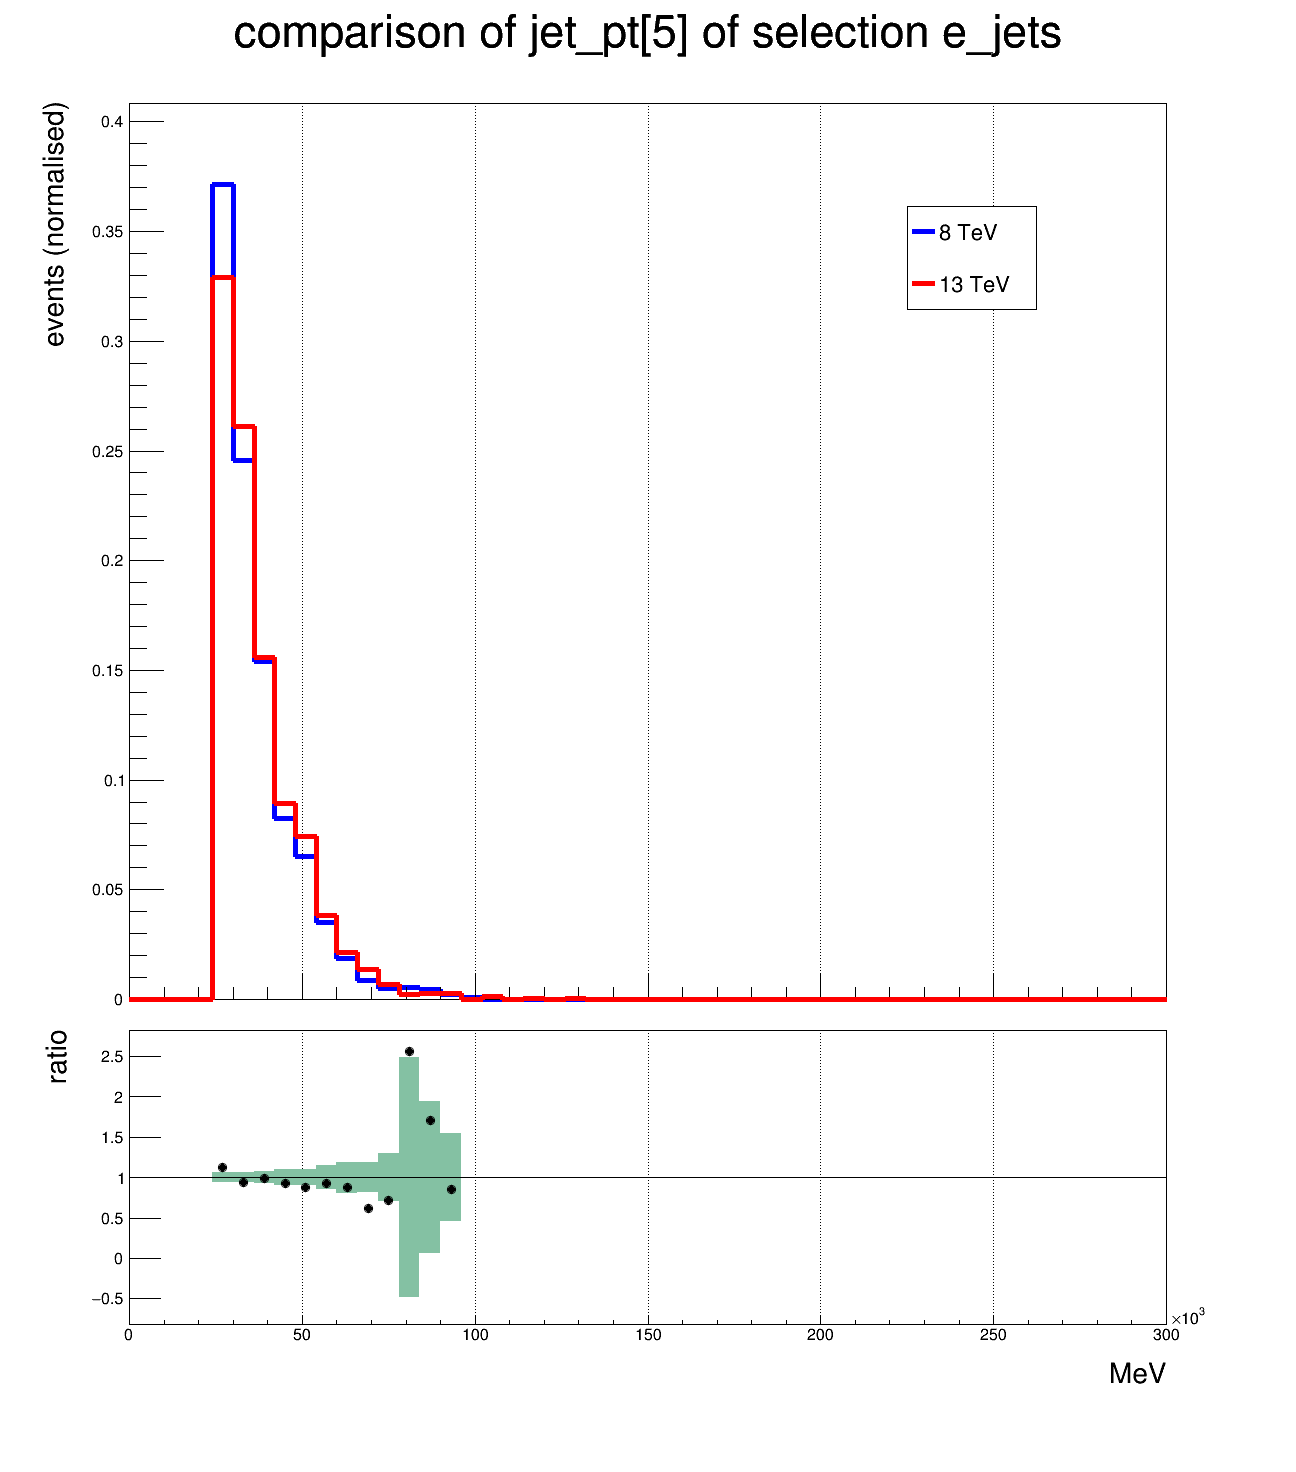
\includegraphics[width=\measureLSpecification]{images_2/2015-04-21T0410Z_comparison_of_jet_pt[5]_of_selection_e_jets.png}\\
\end{tabular}
\end{center}
\end{frame}

\begin{frame}{${p_{T}}$ ratio results for training with epochs of interest}
\begin{table}[h]
\begin{tabular}{cc}
40 epochs:&100 epochs:
\\
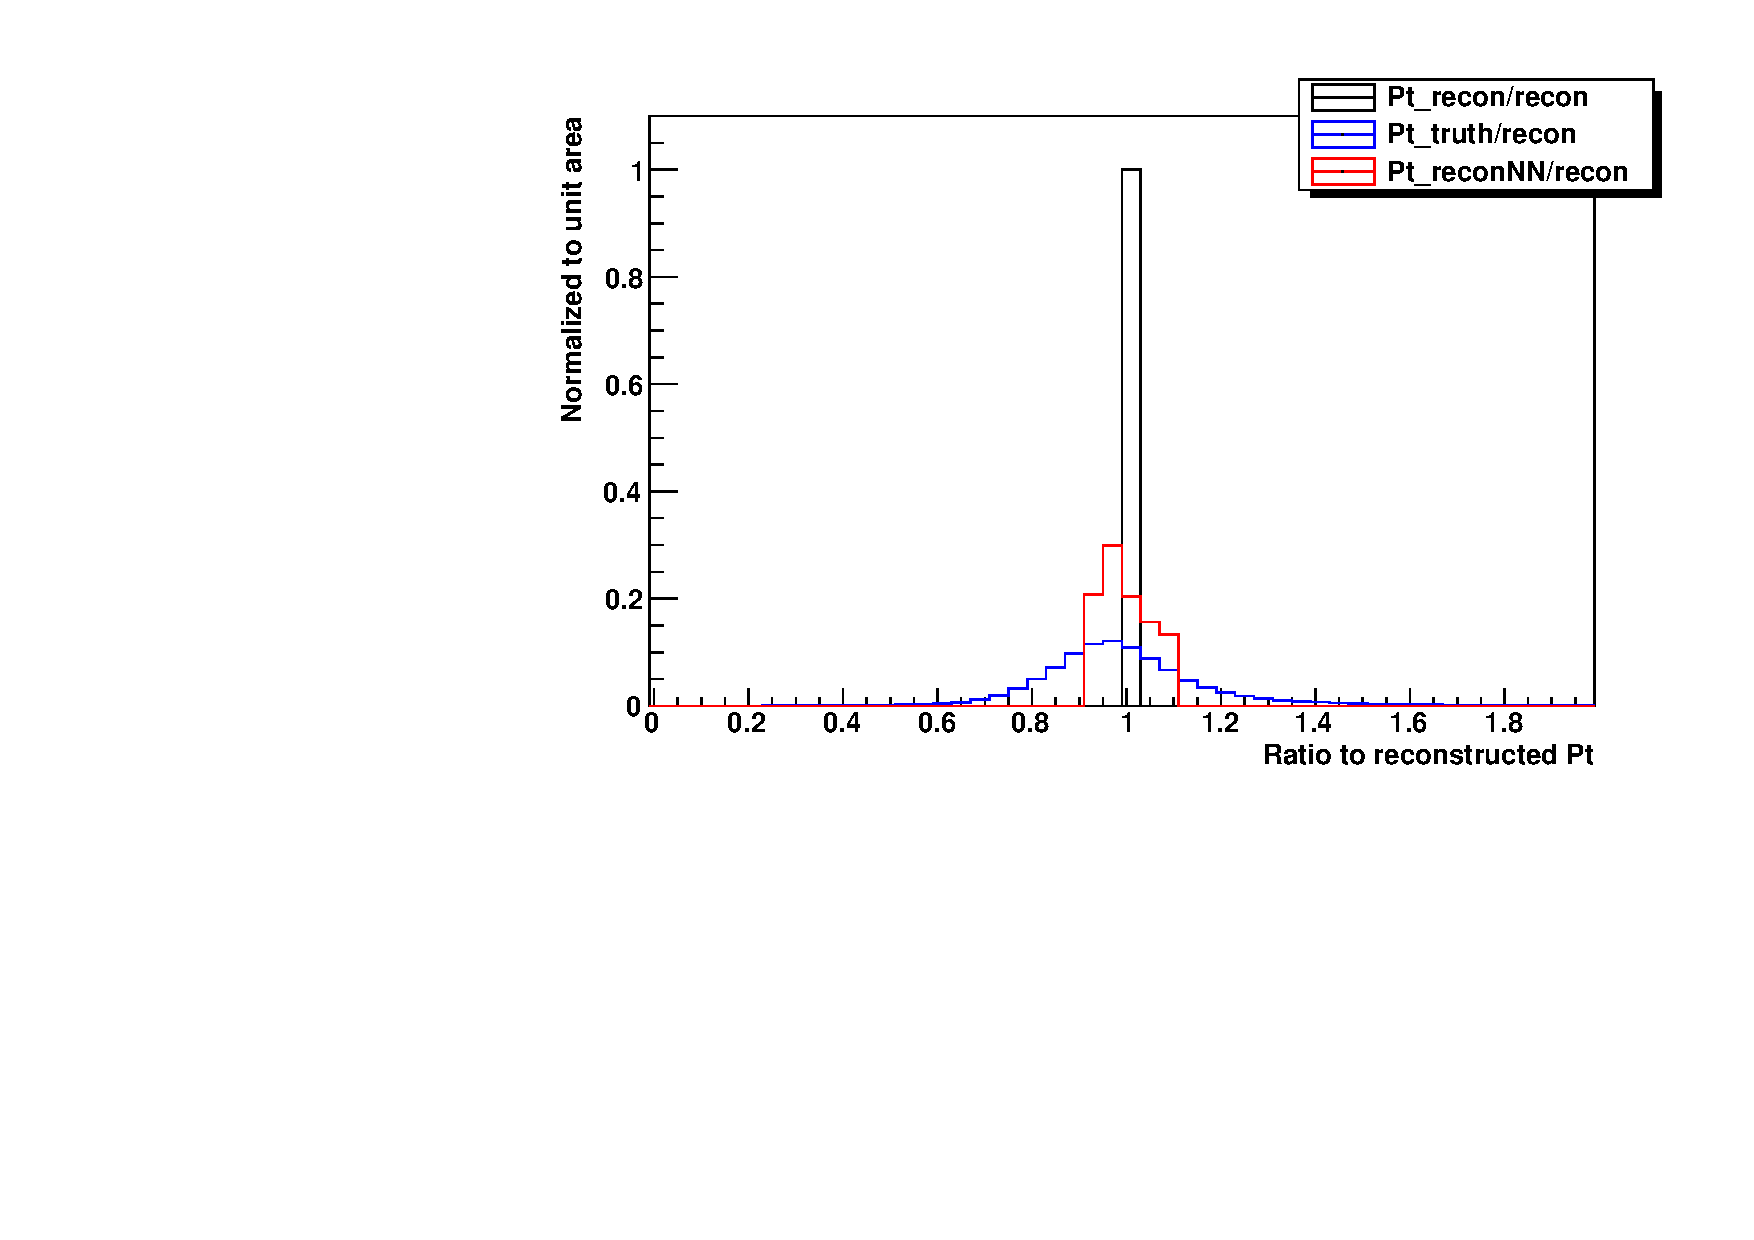
\includegraphics[width=\measureMSpecification]{images_2/wMwN_atlas_125_all_NN_rEt_rSumPtTrk_rWidth5trPt_40_plots_corrected_Pt_train_ratio.pdf}
&
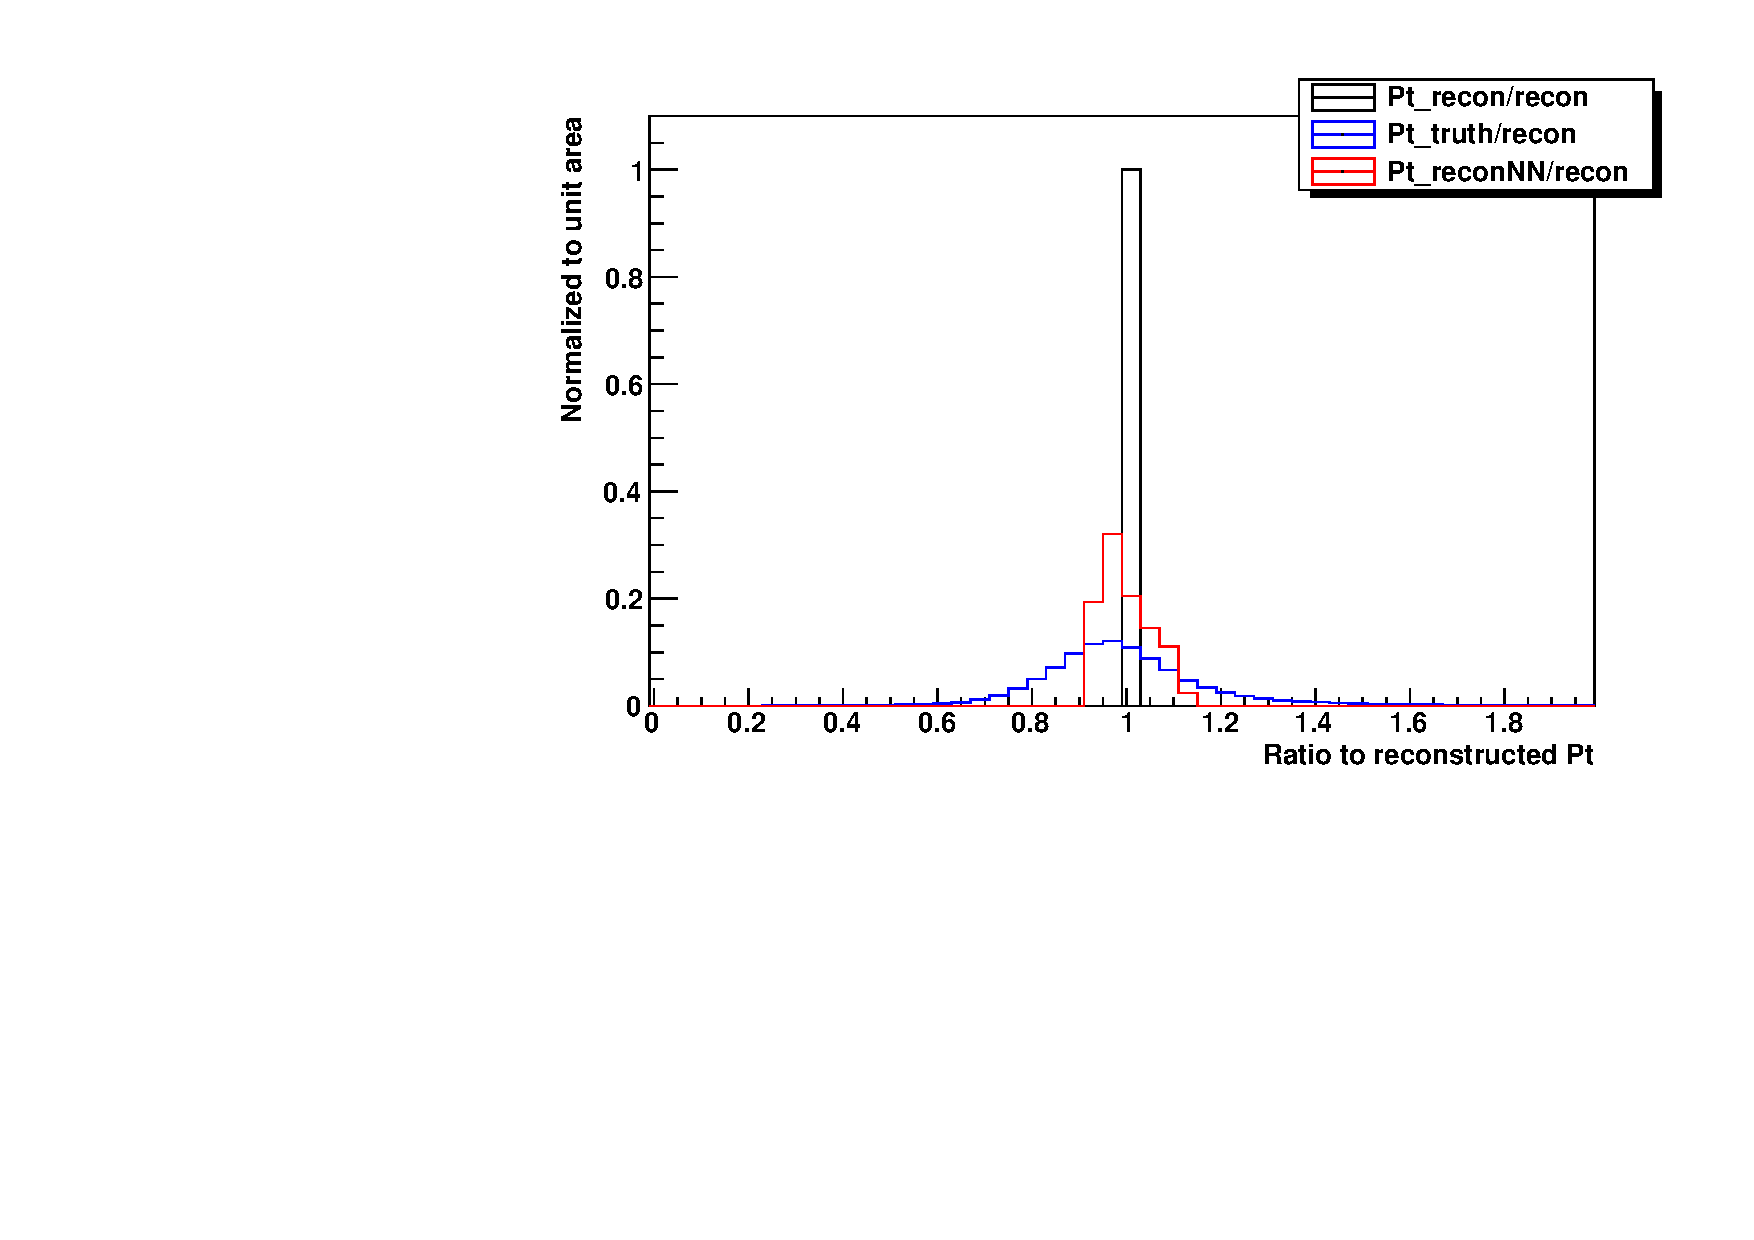
\includegraphics[width=\measureMSpecification]{images_2/wMwN_atlas_125_all_NN_rEt_rSumPtTrk_rWidth5trPt_100_plots_corrected_Pt_train_ratio.pdf}
\\
145 epochs:&300 epochs:
\\
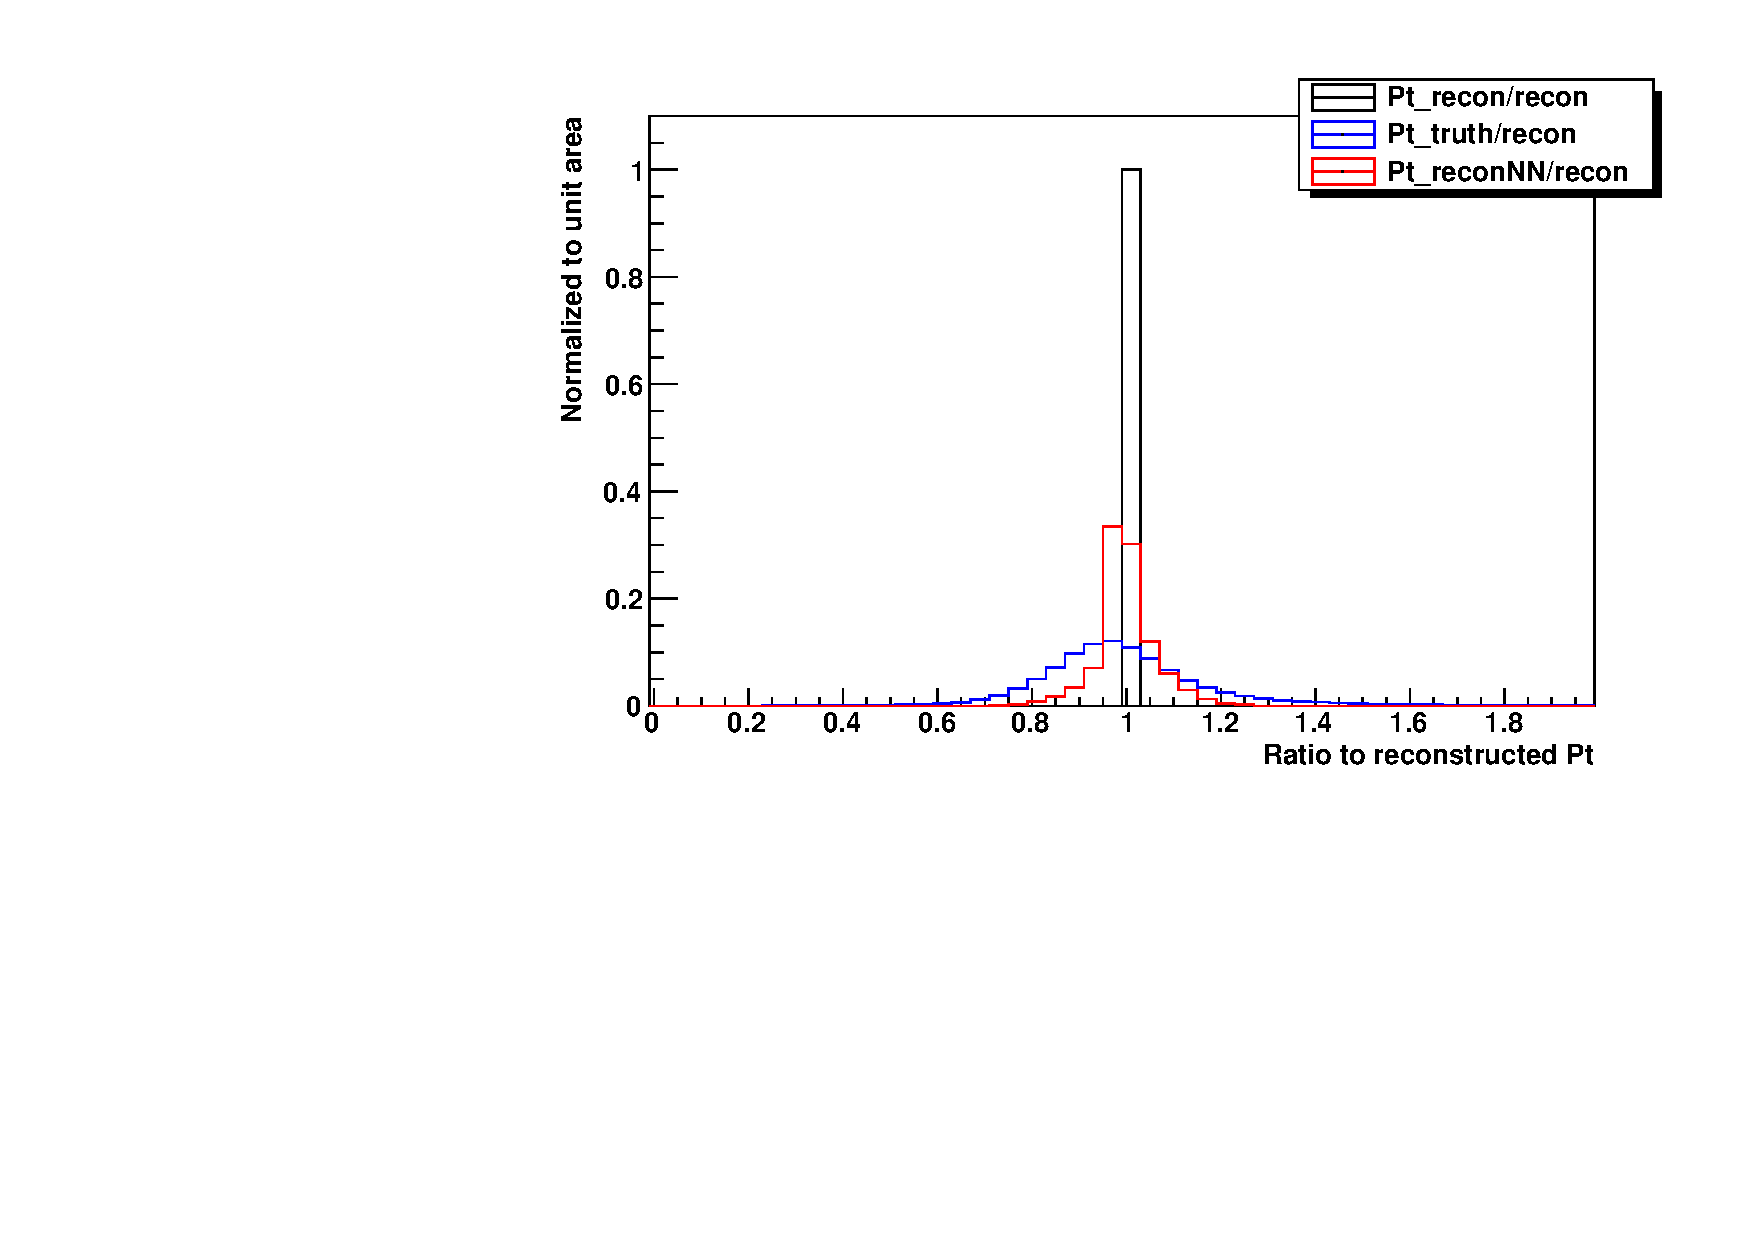
\includegraphics[width=\measureMSpecification]{images_2/wMwN_atlas_125_all_NN_rEt_rSumPtTrk_rWidth5trPt_145_plots_corrected_Pt_train_ratio.pdf}
&
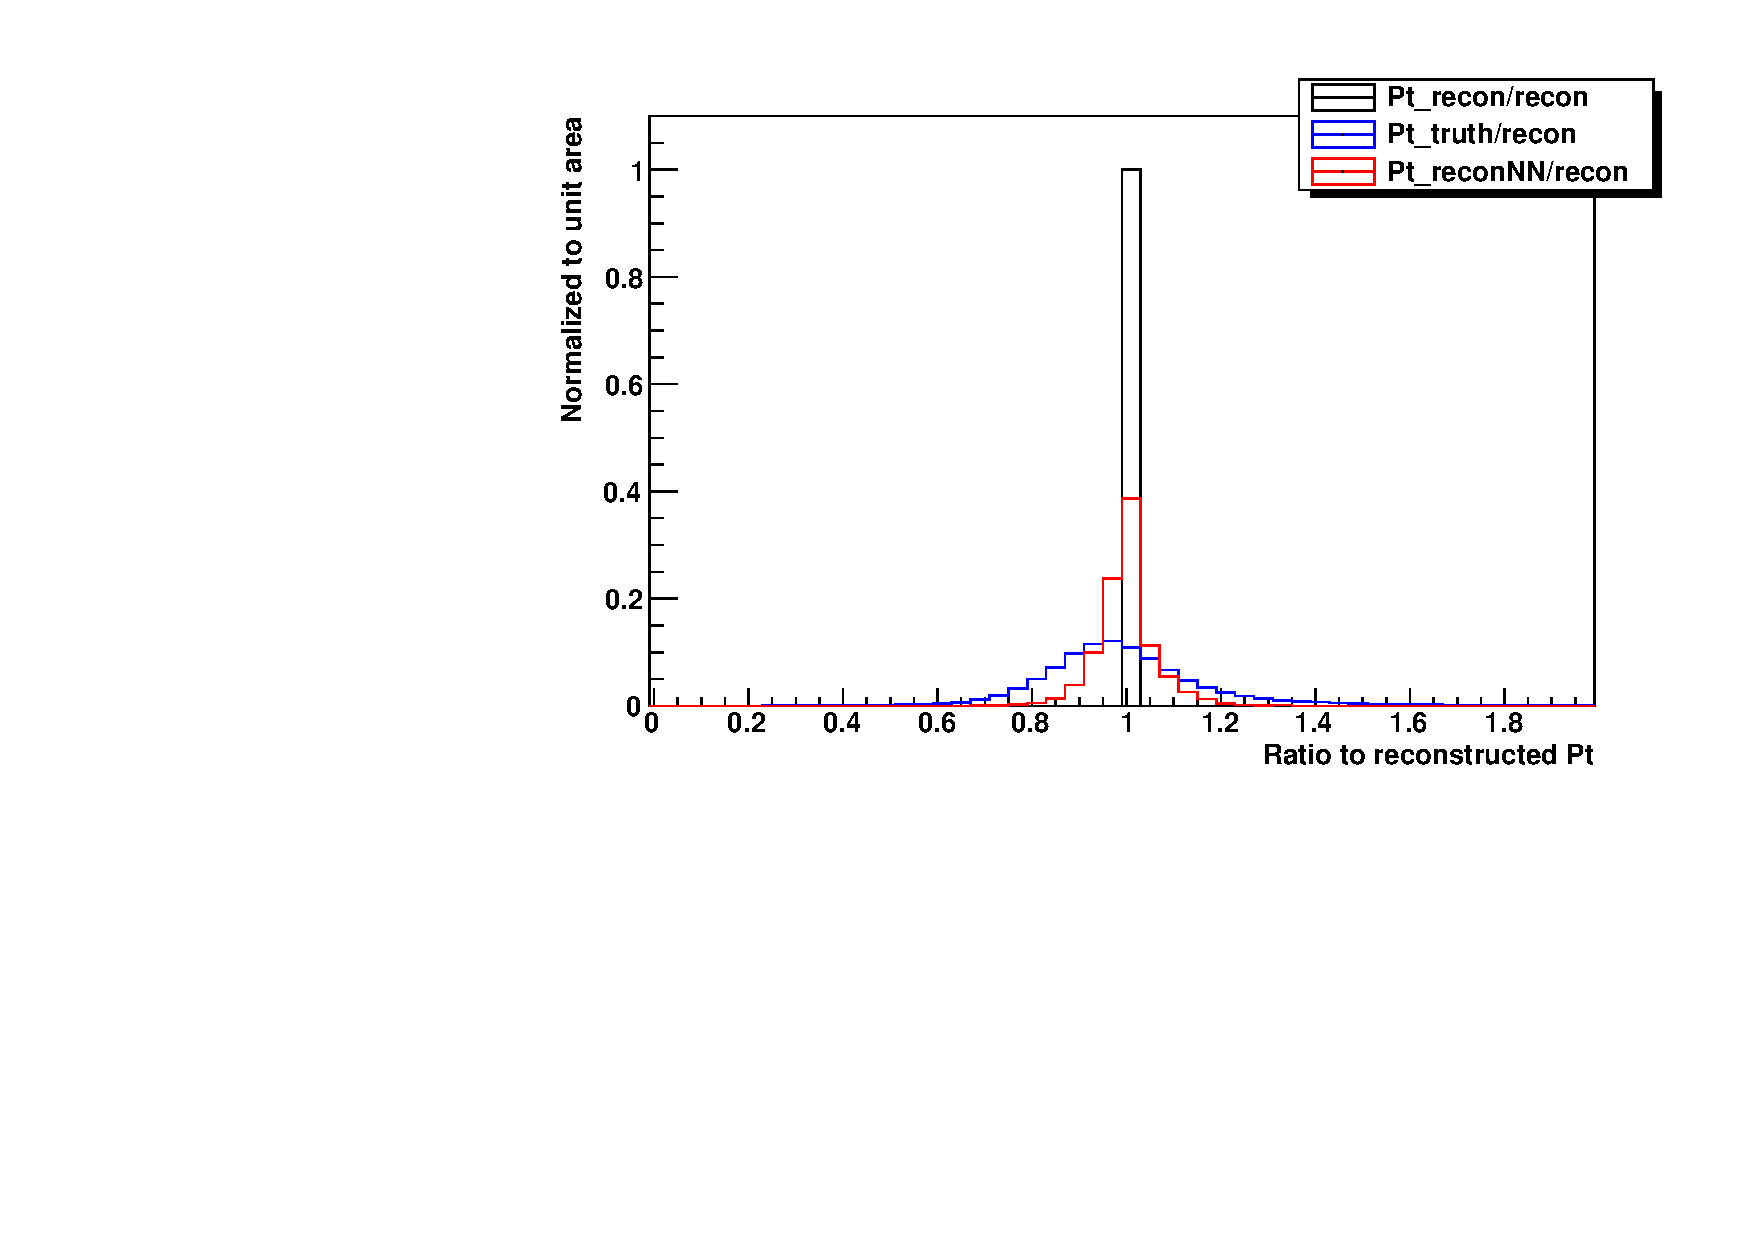
\includegraphics[width=\measureMSpecification]{images_2/wMwN_atlas_125_all_NN_rEt_rSumPtTrk_rWidth5trPt_300_plots_corrected_Pt_train_ratio.pdf}
\\
\end{tabular}
\end{table}
\end{frame}

\begin{frame}{neural networks and input variables}
Four neural networks with progressively increasing input information were defined, all trained through 250 epochs (training cycles). NN0 comprises only the ${\mu}$-in-jet and ${p_{T}}$-only NN corrections, as opposed to further NN corrections.
\begin{center}
\resizebox{11.5 cm}{!}{
\begin{tabular}{ll}
\hline\hline
neural network designation&input variables\\
\hline
NN0&no new neural network applied\\
NN1&Et, SumPtTrk, Width\\
NN2&Et, SumPtTrk, Width, MET\\
NN3&Et, SumPtTrk, Width, MET, METPhi, JetPhi\\
\hline\hline
\end{tabular}
}
\end{center}
\end{frame}

\begin{frame}
\frametitle{per-event $M_{b\bar{b}}$ resolutions with use of MET direction}
${M_{b\bar{b}}}$ resolutions for ${VH_{b\bar{b}}}$ for progressively decreasing MET energy cut requirements for various neural networks, shown to 3 significant figures:
\begin{center}
\resizebox{11.5 cm}{!}{
\begin{tabular}{llllll}
\hline\hline
selection											&	events	&	NN0		& 	NN1		 & 	NN2 		& NN3\\
\hline
${VH_{b\bar{b}}}$									&	23686	&	0.133	&	0.129	&	0.131	&	0.131\\
${VH_{b\bar{b}}+\textrm{MET}<100\textrm{ GeV}}$		&	22654	&	0.132	&	0.130	&	0.129	&	0.131\\
${VH_{b\bar{b}}+\textrm{MET}<70\textrm{ GeV}}$		&	21094	&	0.131	&	0.128	&	0.129	&	0.129\\
${VH_{b\bar{b}}+\textrm{MET}<40\textrm{ GeV}}$		&	15050	&	0.128	&	0.126	&	0.126	&	0.126\\
${VH_{b\bar{b}}+\textrm{MET}<20\textrm{ GeV}}$		&	6174	&	0.130	&	0.127	&	0.126	&	0.127\\
\hline\hline
\end{tabular}
}
\end{center}
\end{frame}

\begin{frame}
\frametitle{per event ${M_{b\bar{b}}}$ resolutions with use of MET direction}
\small Here, the physical processes are ranked according to the effectiveness of the corresponding behaviour they induce in NN3, where a greater effectiveness is taken to mean a smaller resolution value. \emph{Caveat:} Systematic uncertainties are not given their due consideration.
\begin{center}
\resizebox{11.5 cm}{!}{
\begin{tabular}{llllll}
\hline\hline
selection															&	events	&	NN0			& 	NN1			 & 	NN2 		& NN3\\
\hline
\textcolor{red}{${VH_{b\bar{b}}+\textrm{MET}>100\textrm{ GeV}}$}	&	1032	&	0.121542	&	0.129038	&	0.13072		&	\textcolor{red}{0.116975}\\
\textcolor{red}{${VH_{b\bar{b}}+\textrm{MET}<40\textrm{ GeV}}$}		&	15050	&	0.128387	&	0.125939	&	0.125637	&	\textcolor{red}{0.125963}\\				
\textcolor{red}{${VH_{b\bar{b}}+\textrm{MET}<20\textrm{ GeV}}$}		&	6174	&	0.129539	&	0.127454	&	0.126029	&	\textcolor{red}{0.127043}\\
\textcolor{red}{${VH_{b\bar{b}}+\textrm{MET}<70\textrm{ GeV}}$}		&	21094	&	0.131248	&	0.128119	&	0.128908	&	\textcolor{red}{0.128825}\\
\textcolor{red}{${VH_{b\bar{b}}+\textrm{MET}<100\textrm{ GeV}}$}	&	22654	&	0.132004	&	0.129924	&	0.129095	&	\textcolor{red}{0.130467}\\
\textcolor{red}{${VH_{b\bar{b}}}$}									&	23686	&	0.132823	&	0.129032	&	0.131202	&	\textcolor{red}{0.131303}\\
\textcolor{red}{${VH_{b\bar{b}}+\textrm{MET}>20\textrm{ GeV}}$}		&	17512	&	0.135974	&	0.13137		&	0.13366		&	\textcolor{red}{0.132341}\\
\textcolor{red}{${VH_{b\bar{b}}+\textrm{MET}>40\textrm{ GeV}}$}		&	8636	&	0.140116	&	0.135415	&	0.140013	&	\textcolor{red}{0.140551}\\
\textcolor{red}{${VH_{b\bar{b}}+\textrm{MET}>70\textrm{ GeV}}$}		&	2592	&	0.143505	&	0.15228		&	0.151469	&	\textcolor{red}{0.155914}\\
\hline\hline
\end{tabular}
}
\end{center}
\end{frame}

\begin{frame}{${m_{b\bar{b}}}$ value results for training with epochs of interest}
${m_{b\bar{b}}}$ resolution results (Gaussian fit) for training with epochs of interest:
\begin{table}[h]
\begin{tabular}{ll|llll|}
\cline{3-6}
&&\multicolumn{4}{c|}{epochs}\\
\cline{3-6}
&&40&100&145&300\\
\hline
\multicolumn{1}{|l|}{\multirow{2}{*}{subset}}	&training&0.137& 0.138&0.138&0.138\\
\multicolumn{1}{|l|}{}							&training test&0.139&0.139&0.139&0.139\\
\hline
\end{tabular}
\end{table}
\end{frame}

\begin{frame}
\frametitle{${m_{b\bar{b}}}$ resolutions with and without MET}
comparison of ${m_{b\bar{b}}}$ resolutions for various channels both excluding and including the MET variable with various epochs:
\begin{table}[ht]
\centering
\resizebox{9.5 cm}{!}{
\begin{tabular}{|l|l|llll|}
\cline{1-1}\cline{3-6}
number of epochs									&				&	${l\nu bb}$	&	${llbb}$	&	${\nu\nu bb}$	&	all\\
\hline
\multicolumn{1}{|c|}{\multirow{3}{*}{50}}			&	without MET	&	0.135159	&	0.138616	&	0.135159		&	0.137488\\
\multicolumn{1}{|c|}{}								&	with MET	&	0.130047	&	0.137266	&	0.136842		&	0.138516\\
						\cline{2-6}
\multicolumn{1}{|c|}{}								&	change		&	-3.78\%		&	-0.97\%		&	+1.24\%			&	+0.75\%\\
\hline
\multicolumn{1}{|c|}{\multirow{3}{*}{100}}			&	without MET	&	0.134537	&	0.138781	&	0.13656			&	0.13743\\
\multicolumn{1}{|c|}{}								&	with MET	&	0.129719	&	0.137265	&	0.136247		&	0.138948\\
						\cline{2-6}
\multicolumn{1}{|c|}{}								&	change		&	-3.58\%		&	-1.09\%		&	-0.22\%			&	+1.1\%\\
\hline
\multicolumn{1}{|c|}{\multirow{3}{*}{150}}			&	without MET	&	0.13676		&	0.138464	&	0.137943		&	0.13747\\
\multicolumn{1}{|c|}{}								&	with MET	&	0.138292	&	0.137261	&	0.137344		&	0.138948\\
						\cline{2-6}
\multicolumn{1}{|c|}{}								&	change		&	+1.12\%		&	-0.87\%		&	-0.43\%			&	+1.07\%\\
\hline
\multicolumn{1}{|c|}{\multirow{3}{*}{500}}			&	without MET	&	0.139041	&	0.139451	&	0.13849			&	0.13827\\
\multicolumn{1}{|c|}{}								&	with MET	&	0.139225	&	0.137261	&	0.136398		&	0.138948\\
						\cline{2-6}
\multicolumn{1}{|c|}{}								&	change		&	+0.13\%		&	+1.6\%		&	-1.51\%			&	-0.48\%\\
\hline
\end{tabular}
}
\end{table}
\end{frame}

\begin{frame}
\frametitle{embedded data}
\begin{center}
The following is an embedded data file:\\
\mbox{}\\
\textattachfile[color=0 0 0]{embed/data.root}{
    \mbox{\highlightA{\LARGE ${\downarrow}$\Large~data.root}}
}\\
\mbox{}\\
The following is an embedded sound file:\\
\mbox{}\\
\textattachfile[color=0 0 0]{sounds/Omnichord.wav}{
    \mbox{\highlightA{${\tapeSymbol}$\Large~Omnichord.wav}}
}\\
\end{center}
\end{frame}

\begin{frame}
\frametitle{TTHbbLeptonic development team}
\begin{center}
\resizebox{7 cm}{!}{%
\begin{tikzpicture}
\foreach \i in {1,...,8}
    \draw [path image=\i, color=CERNBlue1] (\i * 45 + 30:1.5) circle [radius=0.5cm];
\end{tikzpicture}
}
\end{center}
\end{frame}

\begin{frame}[fragile]
\frametitle{analysis framework}
\vspace{-0.24 cm}
\begin{center}
\tikzset{
    text=black
}
\tikzstyle{empty} = [
]
\tikzstyle{Rectangle1} = [
    rectangle,
    draw,
    fill=#1!20, % e.g. red!20
    node distance=0.65 cm,
    text width=7 em,
    text centered,
    rounded corners,
    minimum height=4 em,
    minimum width=3 cm,
    thick
]
\tikzstyle{Rectangle2} = [
    rectangle,
    draw,
    fill=#1!20, % e.g. red!20
    node distance=1.5 cm,
    text width=7 em,
    text centered,
    rounded corners,
    minimum height=4 em,
    minimum width=3 cm,
    thick
]
\tikzstyle{Diamond} = [
    diamond,
    draw,
    fill=#1!20, % e.g. red!20
    node distance=1.5 cm,
    text width=7 em,
    text badly centered,
    inner sep=0pt,
    thick
]
\tikzstyle{Ellipse} = [
    ellipse,
    draw,
    fill=#1!20, % e.g. red!20
    node distance=1.5 cm,
    text width=7 em,
    thick
]
\tikzstyle{container} = [
    rectangle,
    draw,
    inner sep=0.2 cm,
    dashed
]
\tikzstyle{line} = [
    draw,
    -latex',
    thick
]
\resizebox{6 cm}{!}{%
\begin{tikzpicture}[auto]

    \node [empty](origin){};
    \node [Rectangle1=red, right=of origin](primaryxAODData){
        primary xAOD data
    };
    \node [Rectangle1=red, left=of origin](primaryxAODMC){
        primary xAOD MC
    };
    \node [Rectangle2=blue, below=of origin](DxAOD0And1Lepton){
        DxAOD\\0 and 1 lepton
    };
    \node [Rectangle2=blue, left=of DxAOD0And1Lepton](DxAODMC){
        DxAOD\\MC (also called TOPQ1)
    };
    \node [Rectangle2=blue, right=of DxAOD0And1Lepton](DxAOD2Leptons){
        DxAOD\\2 leptons
    };
    \node [Rectangle2=yellow, below=of DxAOD0And1Lepton](AnalysisTopPackage){
        AnalysisTop package\\TTHbbLeptonic
    };
    \node [Rectangle2=blue, below=of AnalysisTopPackage](Mini-xAODorflatn-tuple){
        Mini-xAOD or flat n-tuple
    };
    \node [Rectangle2=green, below=of Mini-xAODorflatn-tuple](plots){
        plots
    };

    \node [container, fit=(primaryxAODData)(origin)(primaryxAODMC)](container1){
    };
    \node [container, fit=(AnalysisTopPackage)](container2){
    };
    \node [container, fit=(plots)](container3){
    };
    
    \path [line] (primaryxAODMC) -- (DxAODMC) node[pos=0.7, left]{
        event slimming~~
    };
    \path [line] (primaryxAODData) -- (DxAOD0And1Lepton) node[pos=0.7, left]{
        TOPQ1~~
    };
    \path [line] (primaryxAODData) -- (DxAOD2Leptons) node[pos=0.7, right]{
        ~~TOPQ2
    };

    \path [line] (DxAODMC) -- (AnalysisTopPackage);
    \path [line] (DxAOD0And1Lepton) -- (AnalysisTopPackage);
    \path [line] (DxAOD2Leptons) -- (AnalysisTopPackage);

    \path [line] (AnalysisTopPackage) -- (Mini-xAODorflatn-tuple);
    \path [line] (Mini-xAODorflatn-tuple) -- (plots) node[pos=0.5, right]{
        scripts
    };

    \node at (container1.north)[above]{production system};
    \node at (container2.south east)[right]{user grid or local};
    \node at (container3.south east)[right]{user grid or local};

\end{tikzpicture}
}
\end{center}
\end{frame}

\begin{frame}
\frametitle{questions?}
\begin{center}
\resizebox{8 cm}{!}{%
\begin{tikzpicture}
\foreach \i in {1,...,8}
    \pic at (\i * 45 + 30:2.2) {team member=\i};
\node [align=center] {questions?};
\end{tikzpicture}
}
\end{center}
\end{frame}

\begin{frame}
\begin{center}
\mbox{}\\
\Large END
\end{center}
\end{frame}

\end{document}


\end{document}
